\section{INTO-CPS Advanced Method Guidelines}
\label{cha:advanced}

Sections~\ref{sec:method:trace}--\ref{sec:method:dse}, covers more advanced topics that require a basic familiarity with the INTO-CPS technologies. Although Sections~\ref{sec:method:trace}--\ref{sec:method:dse} are ordered based on a start-to-end ``work flow'', it is not necessary to read them in order. Experienced users may read any section on which they require further guidance.

\subsection{Traceability}
\label{sec:method:trace}

The technologies in the INTO-CPS tool chain are able to automatically capture traceability information as activities are performed using the various parts in the tool chain. This includes information about who created or modified an artefact (model, simulation result etc.) and which requirements it is linked to. The traceability features of the INTO-CPS tool are powerful, but require a specific workflow to be followed in order to make best use of them. This chapter explains the steps in this workflow.

This chapter appears first in this advanced material as the following chapters, in particularly Chapters~\ref{sec:reqeng} and~\ref{sec:sysml}, provide key guidance on the first part of the workflow that must be followed in order for traceability to be realised. Those not wishing to use the traceability features can read chapters in any order, driven by their needs or interest. This chapter should be used in conjunction with the User Manual (Deliverable D4.3a~\cite{INTOCPSD4.3a}), which covers details of how to enable traceability recording in the INTO-CPS Application and baseline tools\footnote{Traceability is turned off by default as it can be intrusive if the right workflow is not followed.}. Readers interested in detailed specifications of the traceability and provenance features are directed to Methods Progress Report (Deliverable D3.3b~\cite{INTOCPSD3.3b}), while the tool implementation is described in Deliverables D4.2d~\cite{INTOCPSD4.2d} and D4.3d~\cite{INTOCPSD4.3d}.


\subsubsection{Traceability Workflow}

The INTO-CPS tool chain builds a graph of traceability relations, as there can be multiple relationships between different artefacts. The graph is however tree-like in the sense that there must be some root node(s) to trace from or back too. These root nodes are \emph{requirements}. To use fully the machine-assisted traceability features, it is necessary to initialise the traceability graph by using Modelio from the beginning of the development process. This means that it is necessary to follow these steps:

\begin{enumerate}[noitemsep]
  \item Define requirements through some requirements process (see guidance in Chapter~\ref{sec:reqeng});
  \item Create a Requirements Diagram (RD) in Modelio representing these requirements;
  \item Create an Architecture Structure Diagram (ASD) and Connections Diagram (CD) describing the multi-model;
  \item Link each requirement to one \texttt{<<EComponent>>} (FMU);
  \item Export model descriptions for each \texttt{<<EComponent>>};
  \item Import model descriptions into baseline tools; and
  \item Generate a multi-model configuration from the CD.
\end{enumerate}

After these steps, the traceability graph will then be updated by the baseline tools as models are created from the model descriptions, FMUs are exported and so on, and co-simulation runs and results will be recorded by the INTO-CPS Application. Therefore, by following this workflow it is possible to take advantage of the machine-assisted traceability within INTO-CPS. By performing the required manual input of requirements and links to SysML elements, it is then possible to automatically trace forward to models, FMUs and simulation results, and to trace backwards from these artefacts to individual requirements.

\subsubsection{What Artefacts are Traced?}

%\draftnote{KGP: Our requirements said that we list traced artifacts, so we can quickly summarise the schema here perhaps?}

%\draftnote{CJG: Start by introducing briefly PROV and OSLC relations, which are the basis of the traces}

Traceability in the INTO-CPS tool chain is based upon a study of the actions performed when using the INTO-CPS tool chain, the artefacts that are used and produced and a combination of two existing standards, the W3C's Prov~\footnote{\url{https://www.w3.org/TR/prov-overview/}} and the OMG's OSLC~\footnote{\url{http://open-services.net/}}.   The combination of these resulted in the INTO-CPS traceability ontology that captures in detail all elements in the INTO-CPS workflow and describes the relationships between them.  The complete ontology is presented in deliverable D3.3b~\cite{INTOCPSD3.3b} and a summary is presented here.

Traceability data is inherently a graph based structure based upon nodes and the connections between them, and Prov provides basic types for those nodes along with list of relationships that may exist between them.  The three types of nodes are: Entities, things that may be produced or used during a development process; Activities, are things that act upon and make use of entities; and Agents, objects that have responsibility for entities and activities.  The Prov relations then allow then connection of nodes such as an activity may use an entity, and an entity may be generated by an activity.

The combination of the Prov nodes and relations supports the representation of the processes that lead to the generation of a particular entity, but it does not support connection of those entities to requirements.  OSLC contains a set of specifications, each of which defines a list of relations that it supports between entities. In the case of the INTO-CPS traceability, parts of the OSLC architecture management and requirements management specifications are employed, these allow the connection of entities to requirements via a 'satisfies' relation indicating the entity attempts to address the needs of the requirement, additionally it allows the connection of simulation results to requirements via a 'verifies' relation indicating that the requirement has been met.

%\draftnote{CJG: Introduce that we break the process down into almost atomic actions}

The INTO-CPS traceability ontology breaks the INTO-CPS workflow down into activities that, while not atomic if we consider a user's interaction with a particular tool, could be considered atomic when viewing the process of developing a CPS.  Figure~\ref{fig:traceability:step02} shows the traceability links recorded during one step in the development of a line following robot.  In this example, the requirements, R1 \& R2, already exist in the architecture models and the user has created an ASD to decompose the proposed robot into components.  The user has, at the same time, associated the blocks within the ASD with the the requirements that each block aims to satisfy.  When the user saves the updates architecture model, the Modelio tool records the user's 'Architecture Modelling' activity, along with references to the ASD, the blocks it contains and the newly created links between the blocks and the requirements.  Here the \emph{used}, \emph{wgb} (short for 'was generated by'), \emph{assoc} (short for 'associated with') and \emph{attrib} (short for 'attributed to') are links that come from the Prov standard.  The \emph{OSLC\_Sat} (short for 'satisifies') comes from the OSLC requirements management specification.

%\draftnote{CJG: Give example of one action in detail}

\begin{figure}[htbp]
	\centering
	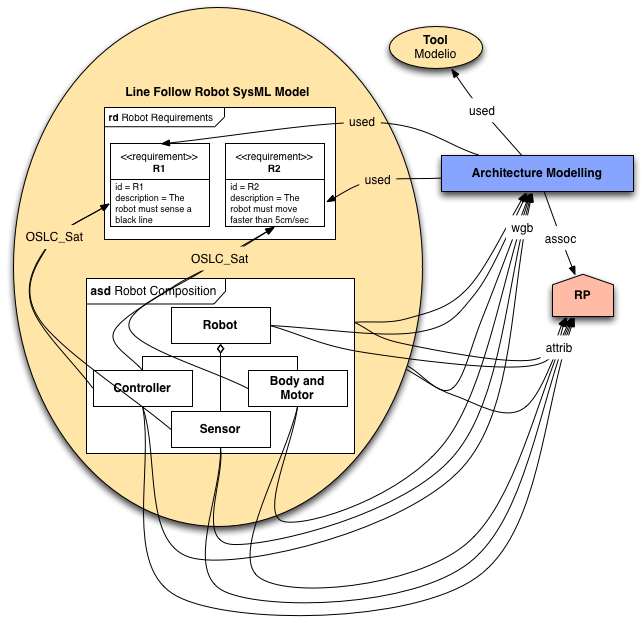
\includegraphics[width=0.8\textwidth]{figures/Traceability/step02}
\caption{Traceability links captured during the production of an ASD for a line following robot.}\label{fig:traceability:step02}
\end{figure}

%\draftnote{CJG: As the user(s) use the tools, they each record the their atomic actions, forming the traceability graph}

A development project will likely consist of many instances of the activities identified in the ontology being performed and together they form a traceability graph.  Figure~\ref{fig:traceability:abstractTraceFlow} shows a simplified view of a traceability graph with some steps removed for brevity.  At the top of the graph we see the architecture modelling step described previously, that produces an architecture model.  From the architecture, model description files are exported to start the production of the simulation models.  In turn the simulation models are exported as FMUs and the FMUs are used to produce simulation results.  Key to the traceability graph then are the 'used' and 'wgb' connections that can be used by a query to determine from where each entity was generated.  By following these links back from any entity to the individual blocks within the architecture model, it is possible to determine which requirement(s) each should satisfy.  Finally when simulation results are output, these may be linked back to the relevant requirements, stating whether a requirement was verified or violated by that result.

%\draftnote{CJG: Give abstract view of a resulting trace}


\begin{figure}[htbp]
	\centering
	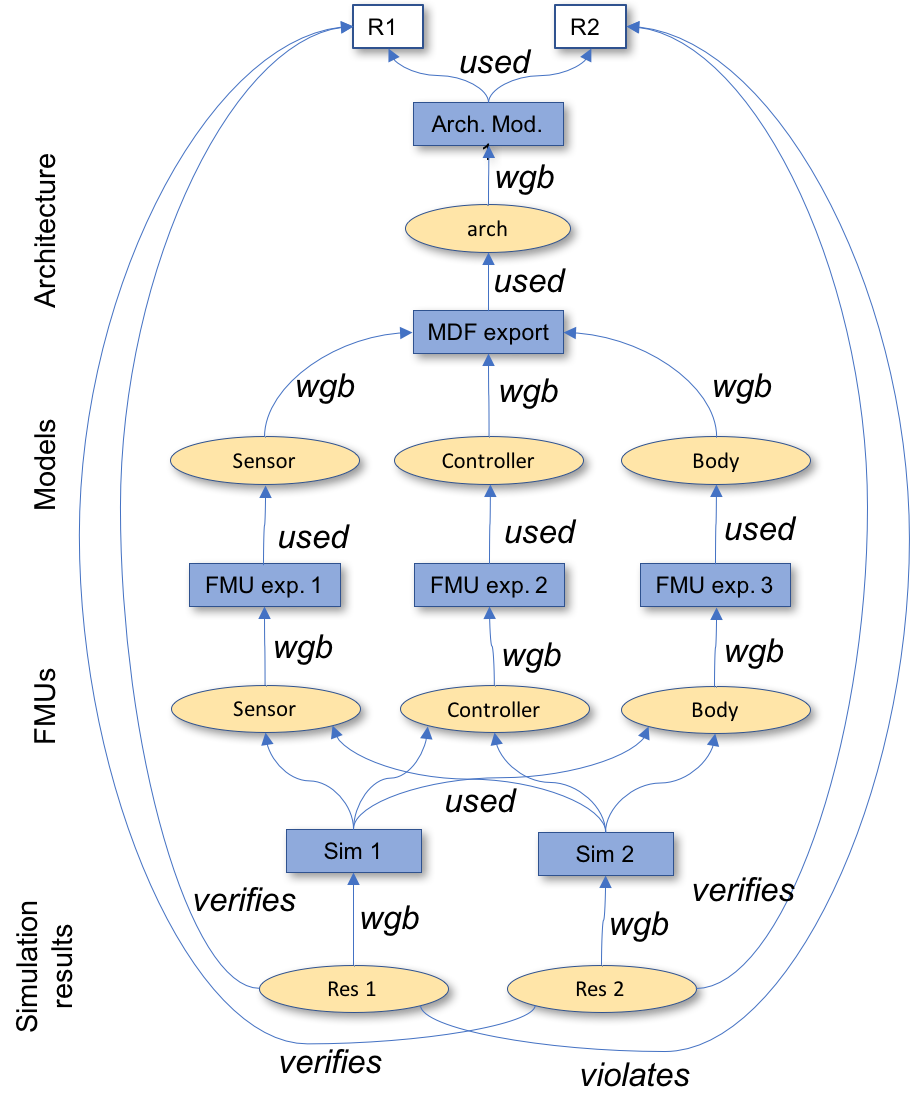
\includegraphics[width=0.7\textwidth]{figures/Traceability/abstractTraceFlow}
\caption{Traceability links captured during the production of an ASD for a line following robot.}\label{fig:traceability:abstractTraceFlow}
\end{figure}


%\draftnote{CJG: A paragraph outlining the entities, activities and agents}

The traceability ontology captures the significant activities and entities that form the INTO-CPS workflow.  For example a development project might see the following activities recorded in the traceability graph:  \emph{Requirements Management}, \emph{Architecture Modelling}, \emph{Architecture Configuration Creation} \emph{Model Description Export}, \emph{Simulation Modelling}, \emph{FMU Export}, \emph{Configuration Creation}, \emph{Simulation Configuration Creation} and then \emph{Simulation}.  These activities are connected in the workflow by the entities they create and use, so the example would see the traceability graph containing records of: \emph{Archtecture Structure Diagram}, \emph{Architecture SubSystem}, \emph{Architecture Connection Diagram}, \emph{Model Description File}, \emph{Simulation Model}, \emph{FMU}, \emph{Multi-model Configuration}, \emph{Simulation Configuration} and \emph{Simulation Result}.  Alongside these will be records of the agent(s), who are both associated with activities and have entities attributed to them.



\subsubsection{Traceability Queries}

%\draftnote{TWT: FMU -> Requirements and Simulation Results -> FMUs are currently implemented.}

The traceability graph created by the INTO-CPS tool chain uses a graph database tool called \emph{Neo4J}. Once a graph has been built, queries can be executed over the graph to perform both forwards and backwards traceability. Below are some types of queries that can be executed over the graphs. The INTO-CPS Application supports some of these queries with the GUI, and the rest through inline access to the Neo4J console.

\begin{enumerate}[noitemsep]
  \item Impact analysis
  \begin{itemize}
    \item Forward traceability (from requirements to entities)
    \item Backwards traceability (from FMU to requirements)
    \item Backwards traceability (from components to requirements)
  \end{itemize}
  \item Simulation sources
  \begin{itemize}
    \item Find all simulations
    \item Find sources and sinks for a simulation
  \end{itemize}
  \item Coverage
  \begin{itemize}
    \item Requirements without architecture elements
    \item Requirements without simulation models
    \item Requirements without FMUs
    \item Requirements without positive simulation results
    \item Requirements without any simulation results
  \end{itemize}
  \item Code sources
  \begin{itemize}
    \item Find all generated source code entities
    \item Find the models for a given source code entity
  \end{itemize}
  \item User impact
  \begin{itemize}
    \item Find all users in the database
    \item Find all artefacts influenced by a user
    \item Find all activities performed by a user
  \end{itemize}
\end{enumerate}

Queries are written in Cypher, a query language built into Neo4J. Advanced users or those developing extensions to INTO-CPS can build their own queries in Cypher\footnote{\url{https://neo4j.com/developer/cypher-query-language/}} and execute them using Neo4J directly as described in the User Manual (Deliverable D4.3a~\cite{INTOCPSD4.3a}).


\subsection{Requirements Engineering}
\label{sec:method:reqeng}

In this chapter, we consider the requirements engineering (RE) activities for the design of CPSs. Specifically, we consider the specification and documentation of requirements placed upon a CPS. These requirements may, for example, impose restrictions, define system capabilities or identify qualities of a system. The requirements should indicate some value or use for the different stockholders of a CPS.

As described in the previous chapter, traceability needs requirements to be defined as early as possible in a development process, and these must be recorded in Modelio for the machine-assisted traceability information to be recorded accurately. It is therefore appropriate to consider requirements processes for such developments at this stage.

In this remainder of this chapter, we discuss the needs for requirements engineering in CPS development, in particular based on the experience of the industrial partners for INTO-CPS. We describe one possible approach to RE for CPS, specifically adapting the SoS-ACRE approach for systems-of-systems (SoSs) to CPS. Note however that this approach is not mandatory, and in general RE processes and tools vary widely across organisations and domains. For this reason, tool support for traceability in INTO-CPS begins once requirements have been defined and can be added to Modelio. The diagrams described in the example are not part of INTO-CPS SysML specification. Therefore, this chapter should truly be treated as guidance, primarily serving to highlight the nature of RE for CPS, which may be of use for both new and more experienced CPS teams.

%In this project, we consider the state in the art of RE in both CPS and Systems of Systems (SoSs), reusing a previously defined approach to RE as applicable.

\subsubsection{Requirements Engineering and Cyber-Physical Systems}

The main issue of concern for RE in CPSs is that of differing domain contexts~\cite{Wiesner&14}. In addition, it has been noted that there are overlaps in challenges in CPSs and SoSs~\cite{Penzenstadler&12}--- especially independence, evolution and, increasingly, distribution. As described by Lewis et al.~\cite{Lewis&09}, as system architectures become more complex, there is often a need to consider requirements and structural architectures during the RE process. The authors suggest that an engineer should identify the system needs, component interactions and stakeholders, and map those needs onto those interested parties. %In Deliverable D3.1b~\cite{INTOCPSD31b}, we also surveyed several projects that had RE as a focus, or part of their focus.

As research in RE in CPS is a nascent field, we suggest one approach is to adopt RE processes from the SoS world, rather than defining an approach specifically for CPSs.  In chapter, we consider SoS-ACRE (System of Systems Approach to Context-based Requirements Engineering)~\cite{Holt&15}, as an example. This approach was adapted from standard systems engineering, and tailored for SoSs--- enabling the identification and reasoning about requirements across constituent systems of an SoS and understanding multi-stakeholder contexts. We suggest it might be useful to organisations trying to approach RE for CPS.
\subsubsection{The SoS-ACRE View of Requirements}

We first consider the collection of views defined in SoS-ACRE, and their applicability to CPS engineering and the INTO-CPS tool chain. These views could be represented as diagrams in SysML\footnote{Note that SoS-ACRE is not specifically supported as a Modelio plug-in, but other equivalent diagrams could be used.}, or as we describe, could equally be represented in other tools where these are already used (e.g. Excel). Examples of each view are shown in Figures~\ref{fig:re-singlesysml}, \ref{fig:re-multisysml}, \ref{fig:re-uri-excel-sysml} and \ref{fig:re-excel-sysml}. %using  technologies relevant to INTO-CPS.

%\fbox{include example figures?}

\begin{description}
\item[Source Element View (SEV)] The SEV defines a collection of source materials from which requirements are derived. In SoS-ACRE, a SysML block definition diagram is considered. In INTO-CPS, this view could also be represented using an Excel table or Word document (with each source having a unique identifier), or by simply referring to source documents using OSLC traces.

\item[Requirement Description View (RDV)] The RDV is used to define the requirements of a system and forms the core of the requirement definition. SoS-ACRE suggests the use of SysML requirements diagram or in tabulated form, such as through the use of Excel. In addition, specifying requirements in  Doors would  support this view.

\item[Context Definition View (CDV)] The CDV is a useful view for CPS engineering in order to explicitly identify interested stakeholders and points of context in the system development, including customers, suppliers and system engineers themselves. In SoS-ACRE, they are defined using SysML block definition diagrams, and could also be represented using an Excel table or Word document (with each context having a unique identifier). This diagram type could be useful when identifying the divide in CT/DE and cyber-physical elements of a system.

\item[Requirement Context View (RCV)] In SoS-ACRE, a RCV is defined for each constituent system context identified in CDVs. This is appropriate when there is a set of diverse system owners, which is typical for SoSs and increasingly CPSs. A \textbf{Context Interaction View (CIV)} is then defined to understand the overlap of contexts and any common/conflicted views on requirements. In a CPS, however, there may not be such a clear delineation between the owners of constituent  system components. However, if we consider the different domains (e.g. CT/DE or cyber/physical divides) as different contexts, then this approach would be useful. In SoS-ACRE, RCVs and CIVs are both defined with SysML use case diagrams. Excel could be used if unique identifiers are defined for contexts and requirements as described earlier.

\item[Validation View (VV)] VVs, defined as SysML sequence diagrams in SoS-ACRE, describe validation scenarios for a SoS to ensure each constituent system context understands the correct role of the requirements in the full SoS. This is not an obvious fit in CPS engineering, and therefore not necessarily required.

\end{description}

\subsubsection{The SoS-ACRE RE Process}

The SoS-ACRE requirement engineering process may be useful for organisations wishing to better understand requirements for CPSm, particularly across multiple domains. It is a lightweight process, and therefore suitable for small- to medium-sized enterprises. Organisations with established may not feel the need to radically alter their existing practice, but may find it instructive to consider how their current processes might be updated or revised to consider better CPS requirements.

% The requirements management is considered to be too heavyweight a target for translation. This is largely due to the fact that we are currently less concerned with requirement change/different processes.

A SoS-ACRE process for CPS should include the following steps:

\begin{enumerate}
\item Identify and record source elements. This would be using a SEV, or simply recording paths to relevant files or documents.

\item Record system-level functional and non-functional requirements. Requirements may be derived using RDVs, and we could consider domain-specific requirements (e.g. cyber or physical), or analysis-specific requirement types (e.g. DSE or testing requirements).

\item Model initial System structure using INTO-CPS ASD. This will identify the cyber and physical elements and the domain/phenomena of the CPS. This may also give initial idea of component functionalities, which may lead to a repeat of Step 2 above\footnote{In the process of architectural modelling, it may also be necessary to redefine contexts depending on whether different simulation tools, or indeed different components of a model, are better able to provide the requirements of the CPS.}.

\item Define the various contexts in CDVs -- both external stakeholders, and if appropriate, contexts for the different components. If only a single system context is defined, then a single RCV is defined. However, if multiple contexts are defined for a CPS, then several RCVs are to be defined, along with a CIV to explore requirements from multiple contexts.

\item Trace the requirements through INTO-CPS tool chain models and results. This was covered in the previous chapter, however we revisit it below in the context of requirements.
\end{enumerate}

\subsubsection{Using technologies with SoS-ACRE}

%In this final section, we consider initial approaches to realise the relevant SoS-ACRE views using the INTO-CPS technologies and those used by industrial partners. This is not expected to constitute final guidelines on this area, as we would make use of INTO-CPS technology currently in development -- namely traceability and provenance support.

As INTO-CPS does not specifically support SoS-ACRE. Indeed INTO-CPS does not mandate and specific approach to RE, because of the wide variety of approaches in industry. We conclude this chapter with an example of how a SoS-ACRE (or other RE process) could be integrated into an INTO-CPS development. We describe a range of permutations of the use of models and documents for recording the requirements engineering process described above. In addition, we include discussions on the links between requirements and architectural models--- identified above as a key method for requirements engineering in CPSs. %We also refer to OSLC and Prov links, which could be linked into the INTO-CPS traceability, though are not supported by the tool chain at the end of the project. Further information on OSLC can be found in Deliverable D3.3b~\cite{INTOCPSD3.3b}.

\begin{description}

\item[URI, Excel and SysML]

We first consider an approach using URIs for the source elements, an Excel document (or a collection of Excel tables) for the RDV, CDV, RCV and CIV of SoS-ACRE. A SysML model in Modelio can be used to define the architecture of the multi-model. Internal tracing in Excel can be achieved using identifiers referenced between sheets. Excel requirements can be replicated in Modelio then traced to elements in the INTO-CPS tool chain automatically. Figure~\ref{fig:re-uri-excel-sysml} presents an example with URI, Excel and SysML models and OSLC links between the artefacts.

\item[Excel and SysML]

The next approach uses Excel to define the SEV and RDV of SoS-ACRE, a SysML model to define the context-oriented views (CDV, RCV and CIV) and a separate architectural model to define the CPS architecture. The Excel requirements can then be mirrored in a Modelio model, and linked to the architectural model. The INTO-CPS traceability features can trace the requirement artefacts to the architectural model. Additional OSLC links could be added manually to link elements of the Excel requirements and context views in a SysML.  Figure~\ref{fig:re-excel-sysml} presents an example with URI, Excel and two SysML models with OSLC links between the artefacts.

\item[Single SysML model]

The next permutation is to use a single SysML model for both requirements engineering and architectural modelling. Such a model will contain all SoS-ACRE views\footnote{Note that Modelio does not currently provide an extension for SoS-ACRE, but these views can be realised using existing SysML stereotypes.} (SEV, RDV, CDV, RCV and CIV), in addition to diagrams defined using the INTO-CPS profile for the CPS composition and connections. Modelling in this way enables trace links to be defined inside a single SysML model. Figure~\ref{fig:re-singlesysml} presents an example SysML model with trace relationships.



\item[SysML requirements and SysML architectural models]

The final permutation is to use SysML for both requirements engineering and architectural modelling, however to use two separate models for the two activities (one containing the RE views (SEV, RDV, CDV, RCV and CIV) and another for architectural diagrams (ASD and CD)). We consider this permutation with two SysML models in addition to the single SysML model, because the requirements engineering and architectural modelling activities are often considered separately, with different engineering teams comprised of engineers with specialist skills. As such we can assume there are cases where these teams have ownership of different models.
Trace links may be used within each individual model (for example, tracing from source elements to requirements in a RE model), and OSLC links defined to trace between requirements elements and architectural elements. Figure~\ref{fig:re-multisysml} presents an example with two SysML models with trace relationships and OSLC links between the models.

\begin{figure}
	\centering
	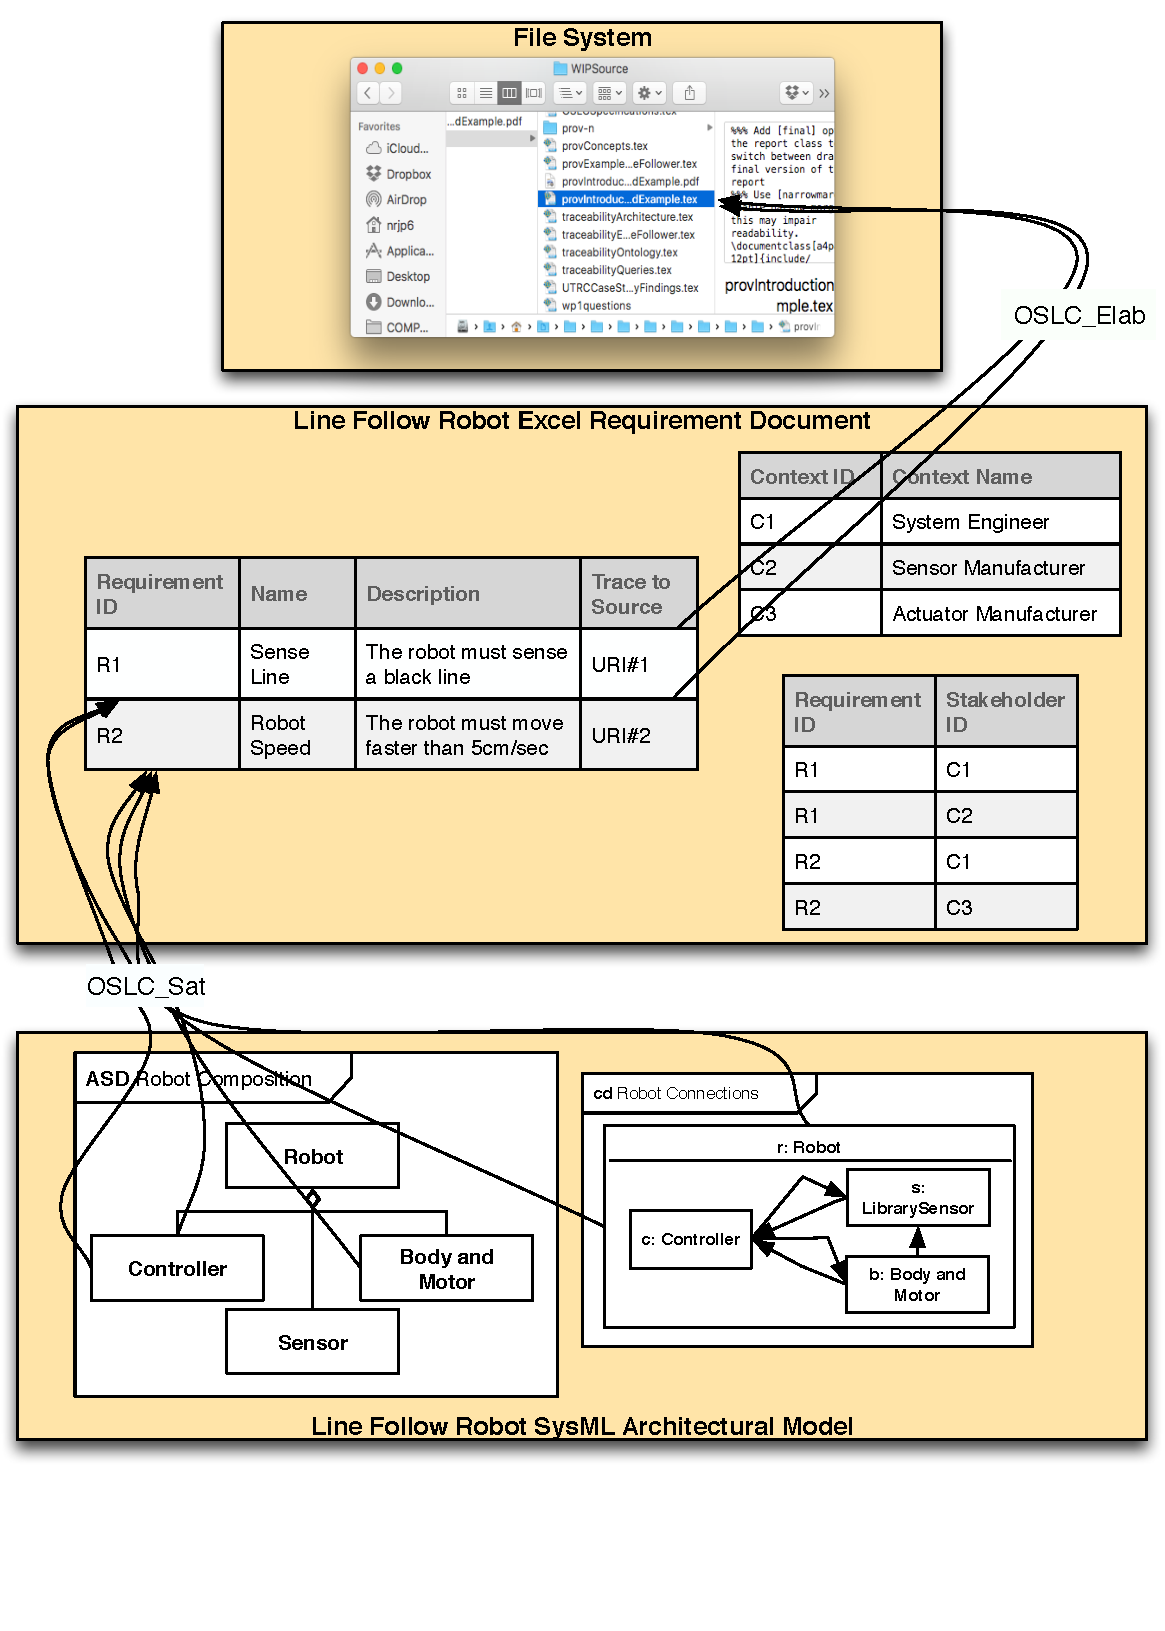
\includegraphics[scale=0.65]{figures/RE_3}
\caption{URI, Excel and SysML -- model overview}
\label{fig:re-uri-excel-sysml}
\end{figure}

\begin{figure}
	\centering
	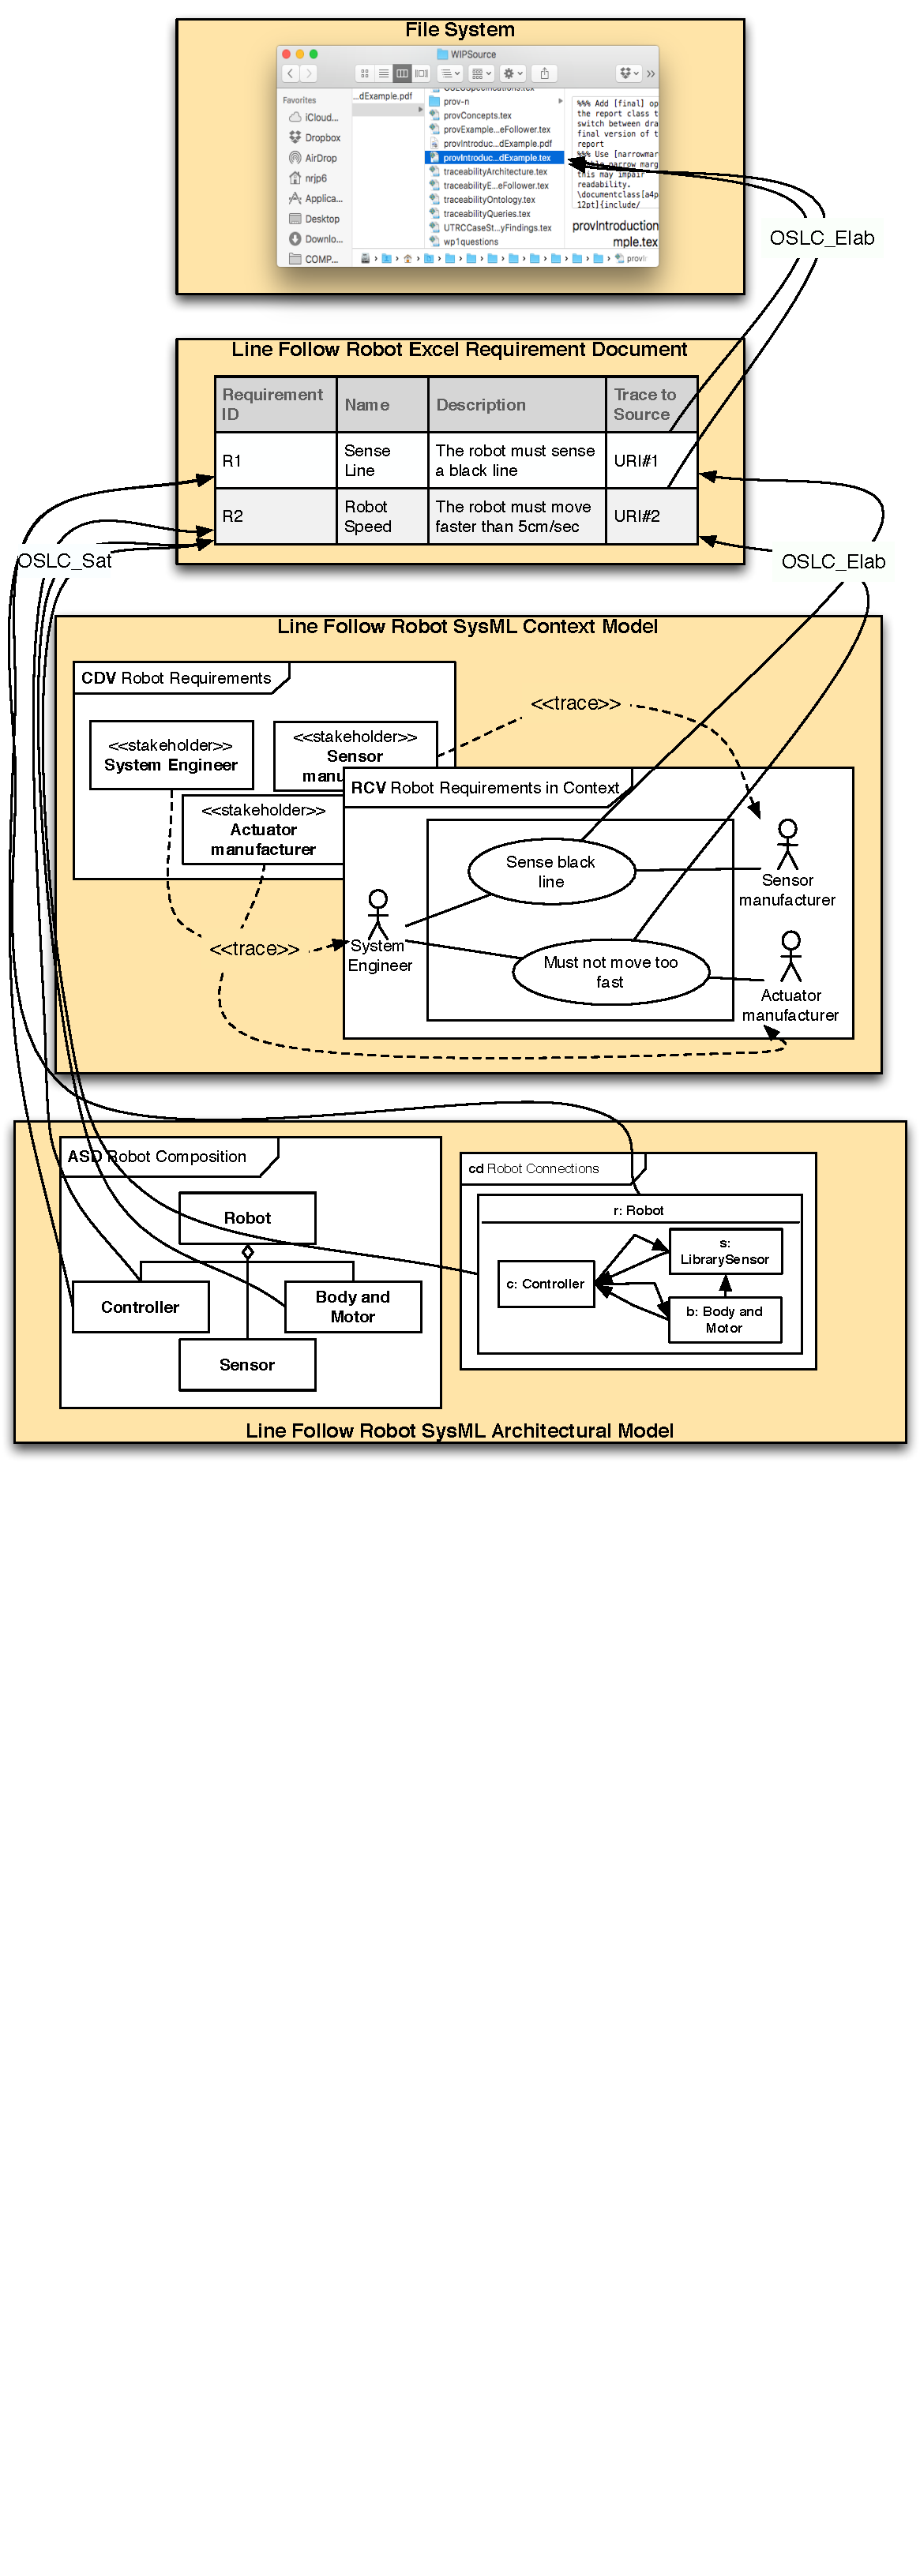
\includegraphics[width=0.8\textwidth]{figures/RE_4}
\caption{Excel and SysML -- model overview}
\label{fig:re-excel-sysml}
\end{figure}

\begin{figure}
	\centering
	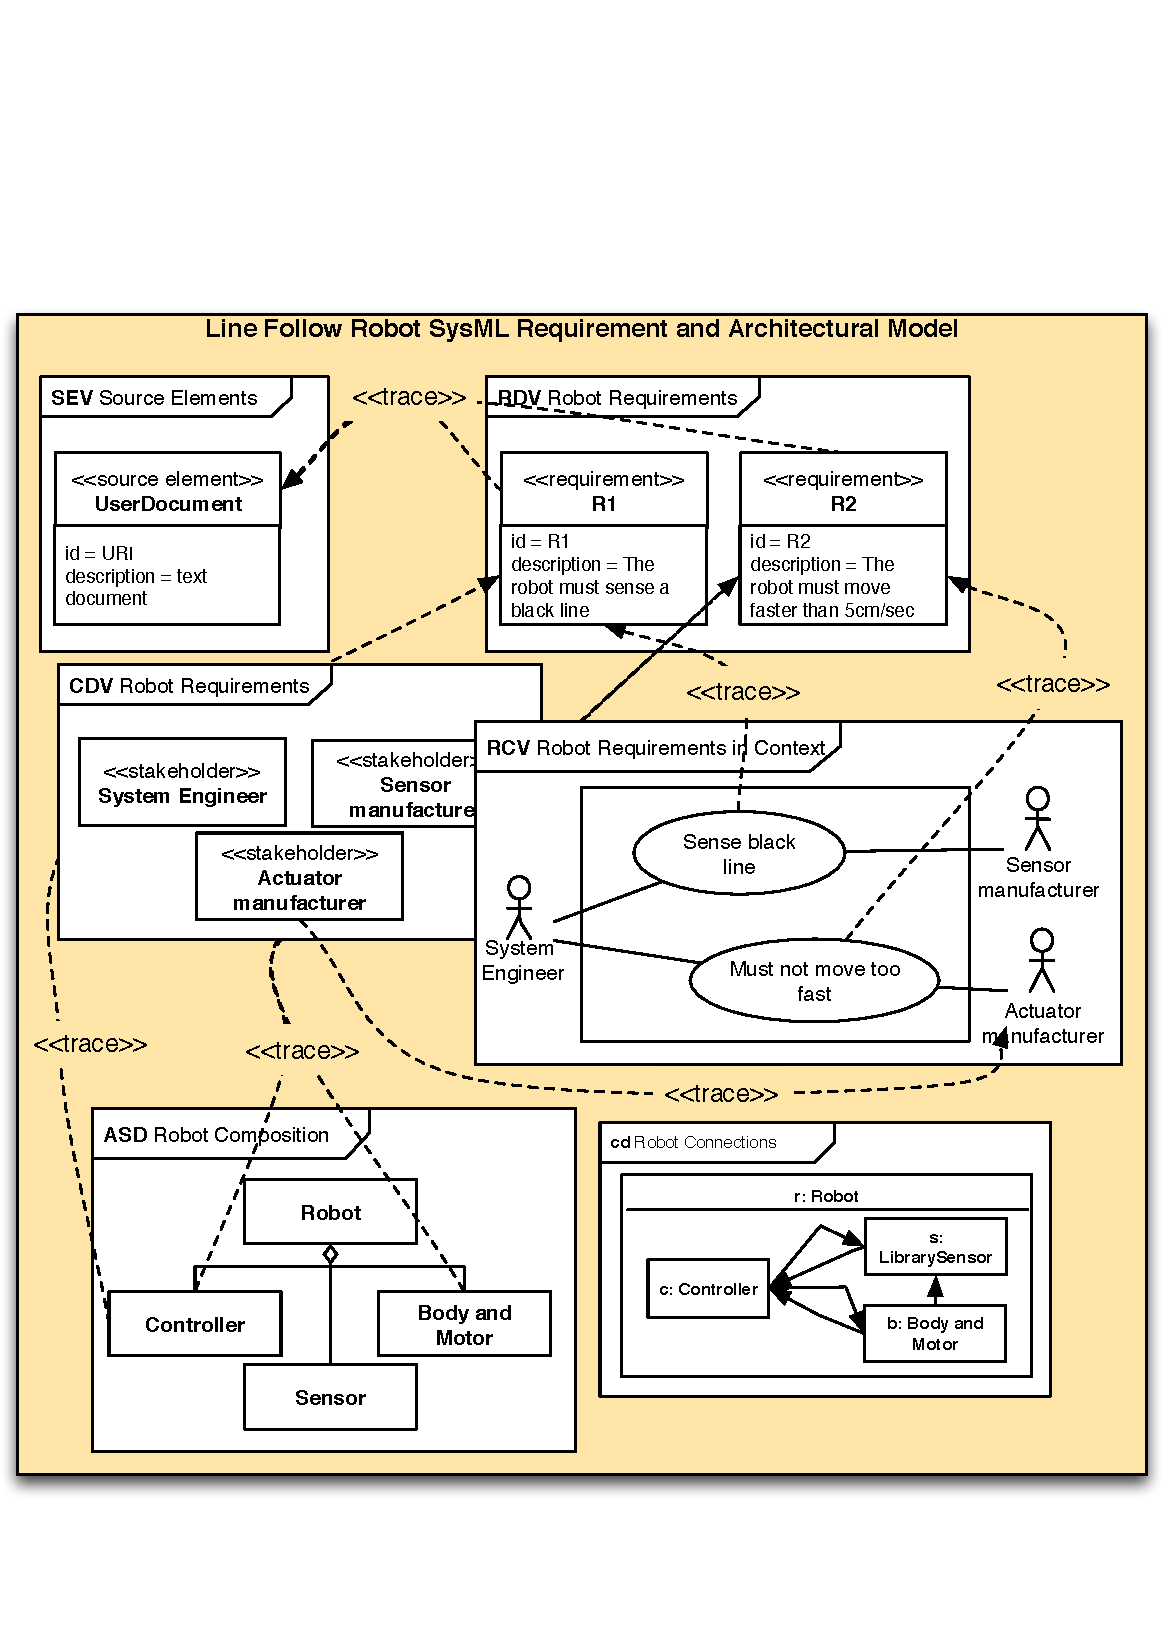
\includegraphics[scale=0.7]{figures/RE_1}
\caption{Single SysML model -- model overview}
\label{fig:re-singlesysml}
\end{figure}

\begin{figure}
	\centering
	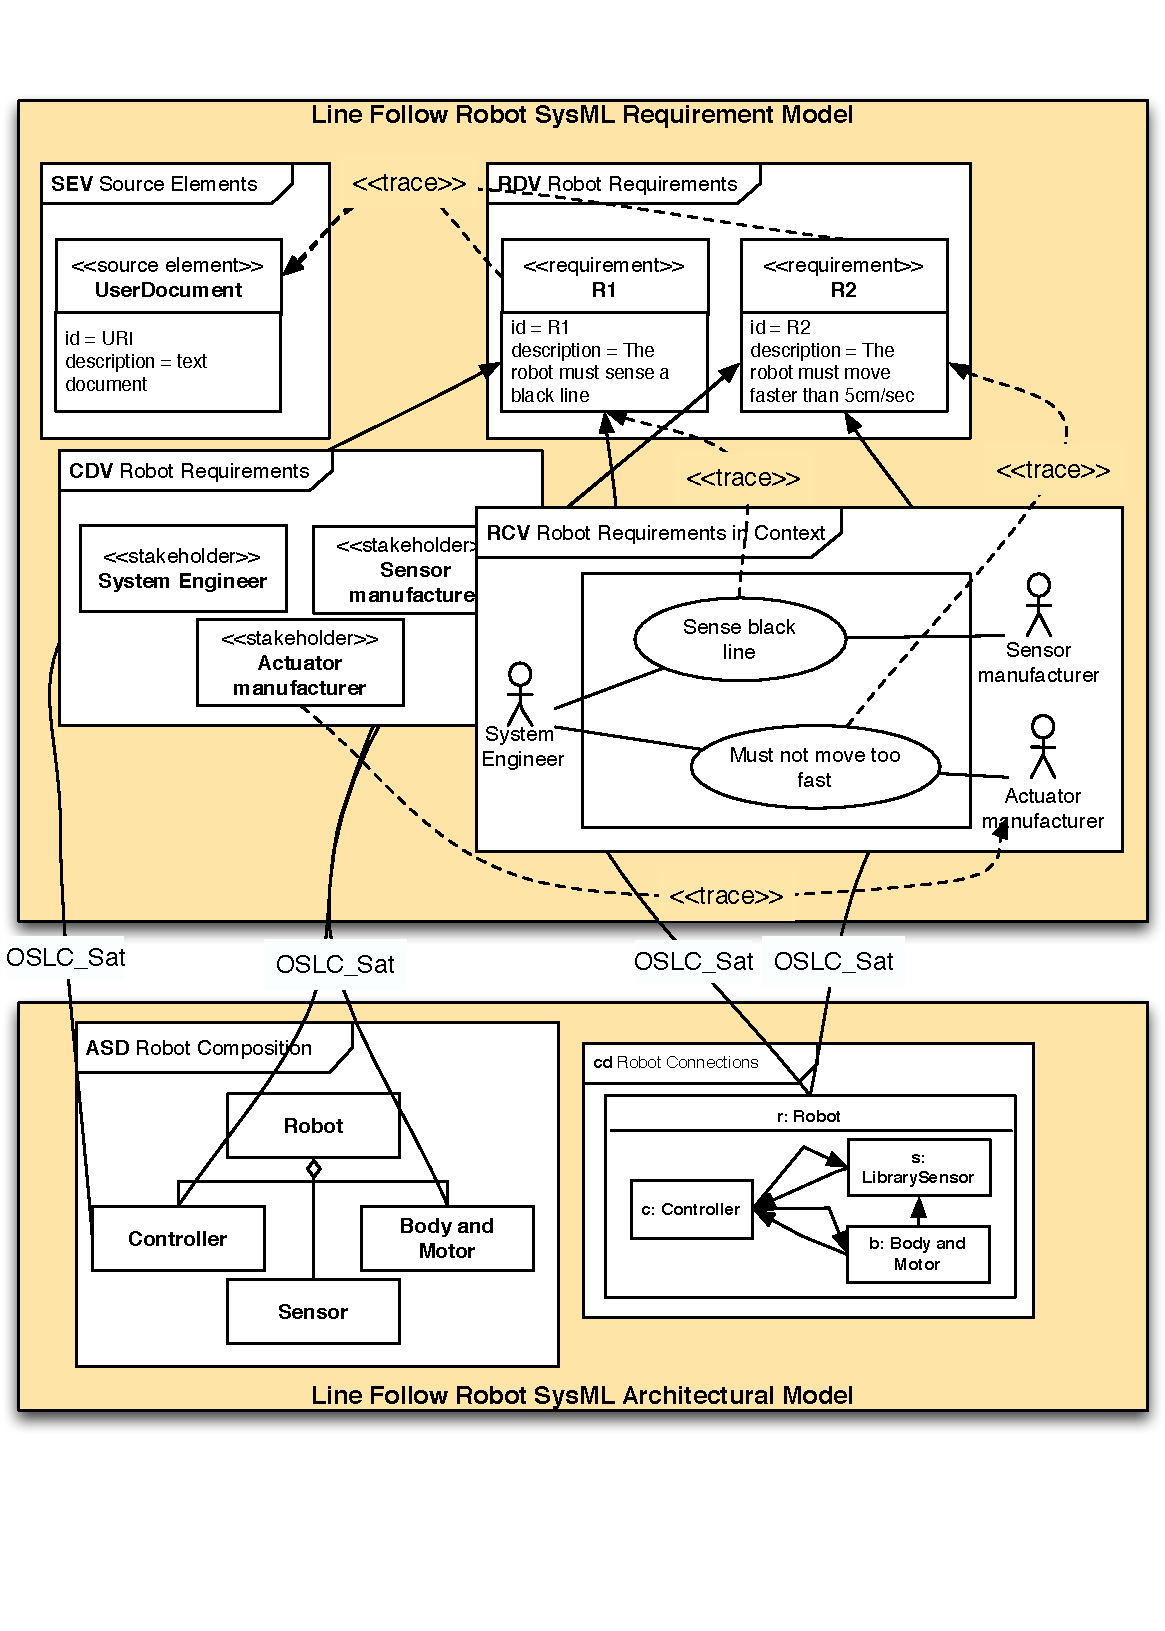
\includegraphics[scale=0.7]{figures/RE_2}
\caption{SysML requirements and SysML architectural models -- model overview}
\label{fig:re-multisysml}
\end{figure}
\end{description}

\subsection{SysML and Multi-modelling}
\label{sec:method:sysml}

This chapter describes the use of SysML with the INTO-CPS tool chain. As described previously in Chapter~\ref{sec:reqeng}, standard SysML can be used as part of a development process to build a model of a system and link elements to requirements. The INTO-CPS tool chain also provides an extended SysML profile that help users to \emph{configure multi-models for co-simulation} and \emph{configure design space exploration (DSE) analysis}~ ~\cite{INTOCPSD2.1a,INTOCPSD2.2a,INTOCPSD2.3a,INTOCPSD41c,INTOCPSD4.2c,INTOCPSD4.3c}. For ease explanation, we describe these separately below, however all the diagrams described are part of a single extended SysML profile.

This chapter summarises the diagrams provided in the two profiles and describe their use in Sections~\ref{sec:sysml:intocps} and~\ref{sec:sysml:dse}. The diagrams presented are illustrative, showing the main elements of a diagram; they are not full definitions of the meta-model, which can be found in the documents cited above. All diagrams are supported by the Modelio tool, and we refer readers to the user manual, Deliverable D4.3a~\cite{INTOCPSD4.3a}, for further information on how to use Modelio to draw these diagrams and generate configurations for use in the INTO-CPS Application.

The chapter concludes with an example of the relationship between a \emph{holistic} model created using standard SysML and a \emph{design} model using the INTO-CPS profile, and concludes with a discussion on how to represent non-design elements (such as FMUs that only perform visualisation) in the INTO-CPS profile in Section~\ref{sec:sysml:non-design}.

\subsubsection{SysML Diagrams Describing Multi-models}
\label{sec:sysml:intocps}

The multi-modelling SysML profile defines two diagrams for configuring a co-simulation. The INTO-CPS Application can run a co-simulation based on a configuration file, using the JSON format to describe the FMUs, their parameters and connections between them. These can be created manually in a text editor, or from the INTO-CPS Application itself. Alternatively, a configuration can be generated by Modelio from the diagrams defined in this profile. There are two types diagram, the \emph{Architectural Structure Diagram} describing the static structure of FMUs, and the \emph{Connections Diagram} describing their instantiation and connections. These are shown in Figure~\ref{fig:sysml:intocps}.

\begin{figure}[h!]
\centering
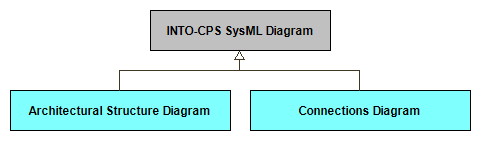
\includegraphics[scale=0.6]{figures/Architecting/ArchitecturalViews}
\caption{Diagrams in the multi-modelling SysML profile}
\label{fig:sysml:intocps}
\end{figure}

\newpage
\paragraph{Architectural Structure Diagram}
\label{sec:sysml:intocps:asd}

The \emph{Architecture Structure Diagram} (ASD) specialises SysML block definition diagrams (BDDs) to support the specification of a multi-model architecture described in terms of a systems components, which will be represented by FMUs. As shown in Figure~\ref{fig:sysml:sysml:intocps:ase} this diagram must include a \texttt{<<System>>} which is then broken down into zero or more \texttt{<<Component>>} blocks.

\begin{figure}[h!]
\centering
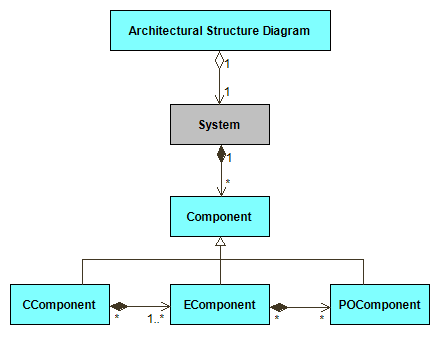
\includegraphics[scale=0.6]{figures/Architecting/ArchitecturalStructureElements}
\caption{\emph{Architectural Structure Diagram} describing FMUs (EComponents) and their hierarchies}
\label{fig:sysml:sysml:intocps:ase}
\end{figure}

There are three types of component block. The \texttt{<<EComponent>>} (encapsulating component) represents a part of a system that will be represented by a single FMU. These blocks have properties indicating which modelling language and tool will be used: \texttt{modelType} (\emph{discrete} or \emph{continuous}) and \texttt{platform} (\emph{VDMRT}, \emph{TwentySim}, \emph{OM}, and \emph{other}).

An \texttt{<<EComponent>>} can be broken down logically into \texttt{<<PComponent>>} (part-of component) representing an internal element of an \texttt{<<EComponent>>}. Both \texttt{<<EComponent>>} and \texttt{<<PComponent>>} blocks can define \emph{variables} and \emph{FlowPorts} that an FMU will have.

The third type of component is a \texttt{<<CComponent>>} (collection component) that allows other components to be grouped logically (it has no ports or behaviours). These can be used to separate design elements within a diagram, as described in Section~\ref{sec:sysml:non-design}. All component blocks have a \emph{kind} that marks their purpose in the model (\emph{cyber}, \emph{physical}, \emph{environment}, \emph{visualisation}).

FMUs are connected by \emph{ports}, and may also present internal state through externally visible \emph{variables}, which can be monitored on a live graph, for example. Both \texttt{<<EComponent>>} and \texttt{<<PComponent>>} blocks can define \emph{FlowPort} and \emph{Variable} attributes, as shown in Figure~\ref{fig:sysml:sysml:intocps:asi}, which will form the interface of the FMU and are added to the ``model description'' exported by Modelio.

\begin{figure}[h!]
\centering
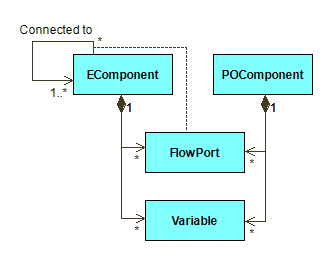
\includegraphics[scale=0.6]{figures/Architecting/ArchitecturalStructureInterfaces}
\caption{Component blocks may define variables and ports}
\label{fig:sysml:sysml:intocps:asi}
\end{figure}

%\begin{figure}[h!]
%\centering
%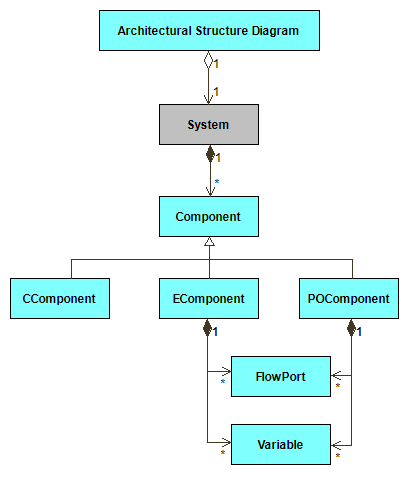
\includegraphics[scale=0.6]{figures/Architecting/ArchitecturalStructureView}
%\caption{\emph{Architectural Structure Diagram} describing connections between FMUs}
%\label{fig:sysml:sysml:intocps:asd}
%\end{figure}

%\clearpage
\paragraph{Connections Diagram}
\label{sec:sysml:intocps:cd}

The \emph{Connections Diagram} (CD) specialises SysML internal block diagrams to convey the internal configuration of the systems components. Specifically, it describes which FMUs are instantiated (i.e. which \texttt{<<EComponent>>}s form the ASD), and how the ports are connected. This diagram is used by Modelio to generate multi-model configurations.

\begin{figure}[h!]
\centering
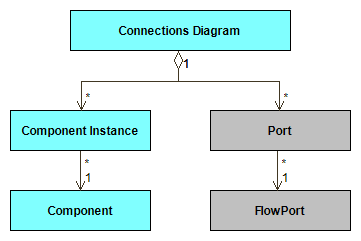
\includegraphics[scale=0.6]{figures/Architecting/ConnectionsView}
\caption{\emph{Connections Diagram} describing the static structure of FMUs}
\label{fig:sysmlintocps:cd}
\end{figure}

\subsubsection{SysML Diagrams Describing Design Space Exploration}
\label{sec:sysml:dse}

The design space exploration (DSE) SysML profile is an addition to the multi-modelling SysML profile described above. As with single co-simulation, the INTO-CPS Application can run a DSE based on a JSON configuration file. These can be created manually in a text editor or edited in the INTO-CPS Application. Alternatively, a configuration can be generated by Modelio, from a set of diagrams defined in the profile. There are five diagram types, which are described below. Further guidance on DSE can be found in Chapter~\ref{sec:dse}.

\begin{figure}[h!]
\centering
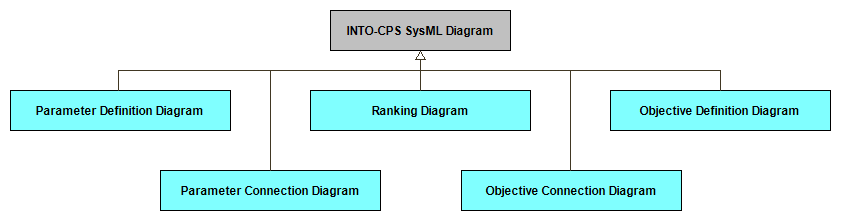
\includegraphics[scale=0.5]{figures/DSE/DSEViews}
\caption{Diagrams in the DSE SysML profile}
\label{fig:sysml:dse}
\end{figure}

\paragraph{Objective Definition Diagram}
\label{sec:sysml:dse:odd}

The \emph{Objective Definition Diagram} is used to define the objectives for use during a DSE. Objectives are characterising measures of performance that may be used to determine the relative benefits of competing designs. They are defined as metrics over the results of a co-simulation of a specific design and are used to judge its quality for use in later processing e.g. ranking.

Objectives are described in terms of a name, a script file that will be used to compute them, and the ports that will provide the data they require. As with the \emph{Architectural Structure Diagram} above (Section~\ref{sec:sysml:intocps:asd}), this diagram gives the static structure of the objectives; instances of these definitions are created using the \emph{Objective Connection Diagram} below (Section~\ref{sec:sysml:dse:ocd}).

\begin{figure}[h!]
\centering
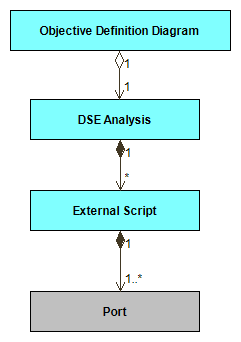
\includegraphics[scale=0.5]{figures/DSE/ObjectiveDefinitionView}
\caption{\emph{Objective Definition Diagram} describing objectives in a DSE}
\label{fig:sysml:sysml:dse:odd}
\end{figure}

\paragraph{Objective Connection Diagram}
\label{sec:sysml:dse:ocd}

The \emph{Objective Connection Diagram} is used to instantiate objectives defined in the \emph{Objective Definition Diagram} above (Section~\ref{sec:sysml:dse:odd}). The diagrams allow the ports of each instance of the objective to be linked to a data source: either a static value, or a value from data exchanged in the multi-model.

\begin{figure}[h!]
\centering
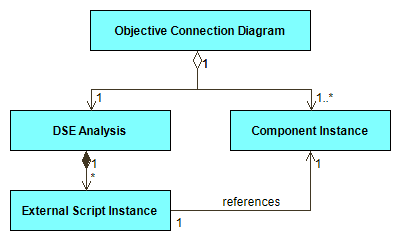
\includegraphics[scale=0.5]{figures/DSE/ObjectiveConnectionsView}
\caption{\emph{Objective Connections Diagram} linking objectives to data sources}
\label{fig:sysml:sysml:dse:ocd}
\end{figure}

\paragraph{Parameter Definition Diagram}
\label{sec:sysml:dse:pdd}

The \emph{Parameter Definition Diagram} is used to define the parameters that will changed for each co-simulation in a DSE. Parameters are described in terms of a name, and a set of values that we wish to test. The product of the cardinalities of the set of values for each parameter gives the size of the design space--- the total number of simulation required for an exhaustive search. As with the \emph{Architectural Structure Diagram} above (Section~\ref{sec:sysml:intocps:asd}), this diagram gives the static structure of the parameters; instances of these definitions are created using the \emph{Parameter Connection Diagram} below (Section~\ref{sec:sysml:dse:pcd}).

\begin{figure}[h!]
\centering
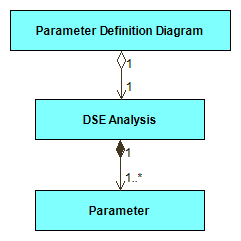
\includegraphics[scale=0.5]{figures/DSE/ParameterDefinitionView}
\caption{\emph{Parameter Definition Diagram} defining parameters and their values}
\label{fig:sysml:sysml:dse:pdd}
\end{figure}

\paragraph{Parameter Connection Diagram}
\label{sec:sysml:dse:pcd}

The \emph{Parameter Connection Diagram} is used to instantiate parameters defined in the \emph{Parameter Definition Diagram} above (Section~\ref{sec:sysml:dse:pdd}). The diagram allows the parameters to be linked to those provided by the FMUs in the multi-model.

\begin{figure}[h!]
\centering
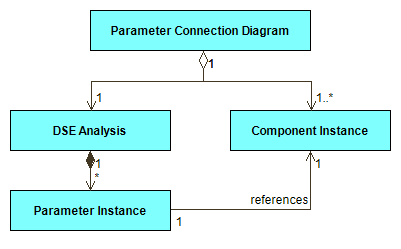
\includegraphics[scale=0.5]{figures/DSE/ParameterConnectionsView}
\caption{\emph{Parameter Connections Diagram} linking parameters to FMUs}
\label{fig:sysml:sysml:dse:pcd}
\end{figure}

\paragraph{Ranking Diagram}
\label{sec:sysml:dse:rd}

The \emph{Ranking Diagram} is used to declare which of the objectives should be used to compare competing designs, and whether lower or higher values for each the objectives is better (i.e. whether to maximise or minimise a value).

\begin{figure}[h!]
\centering
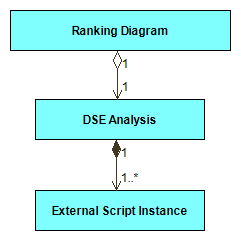
\includegraphics[scale=0.5]{figures/DSE/RankingView}
\caption{\emph{Ranking Diagram} defining how to rank designs based on objectives}
\label{fig:sysml:sysml:dse:rd}
\end{figure}


\subsubsection{Holistic and Design Architectural Modelling}
\label{sec:sysml:holistic}

A system architecture defines the major components of a system, and identifies their relationships, behaviour and interactions. A model of the architecture is potentially partial (representing some or all of the system) and abstract, limited to those elements pertinent to the modelling goal. In CPS engineering, this goal may include understanding the system in terms of the application domain (a \emph{holistic} model), or capturing the system components in a way that targets multi-modelling (a \emph{design} model).

The diagrams in the two profiles described above divide architectural models into subsystems composed of cyber or physical components. Defining an architecture this way may not be the best approach when designing a system ab initio, with systems comprising entities across different domains requiring diverse domain expertise. Following on from Chapter~\ref{sec:reqeng}, this section uses a smart grid example to show both holistic and design architectural modelling approaches, and provide some commentary and guidance on how to model in a way which is natural for domain experts, and how to move from holistic to design models when multi-modelling.

\paragraph{Example Introduction}

%\fbox{mention what a SG is briefly:  control, distributed control, ideas of power gen, transmission, substations etc}
A smart grid is an electricity power grid where integrated ICT systems play a role in the control and management of the electricity power supply. Such ICT elements include distributed control in households, control of renewable energies and networked communications.
In this section we outline a Smart Grid\ model to explore different design decisions in the cyber control of an electricity power grid. The model presented here is a small illustrative example, which omits complexities of a real Smart Grid. For example, the change from three-phase AC power to one-phase DC power allowing us to use simpler physical models. A second simplification is in the number of houses present in the grid model. We model only 5 houses, assumed to be in a small local area supplied by a single substation. We do not consider the remainder of the grid. To ensure that any effect due to changes in the power consumption by those properties are observed by the other houses, we skew the resistance of the transmission lines between the power generation and substation, and substation to houses.

\paragraph{Holistic Architectural Model}

A Block Definition Diagram (BDD) of the Smart Grid is given in Figure~\ref{fig:bdd}. The figure shows that the \textit{Smart Grid} system comprises two top-level physical elements: \textit{Power Generation} and \textit{Transmission Lines}; a single top-level cyber elements: the \textit{Data Network}; and two cyber-physical systems: a \textit{Substation} and several \textit{Houses}. The two elements may be further decomposed. The \textit{Substation} elements is composed of a cyber \textit{Substation Controller} and physical \textit{Substation Meter} and \textit{Step-down Transformer}. The \textit{House} element comprises: a cyber \textit{House Controller}, physical \textit{House Meter} and \textit{Devices}, and an \textit{Owner/Usage Profile}.

\begin{figure}
\centering
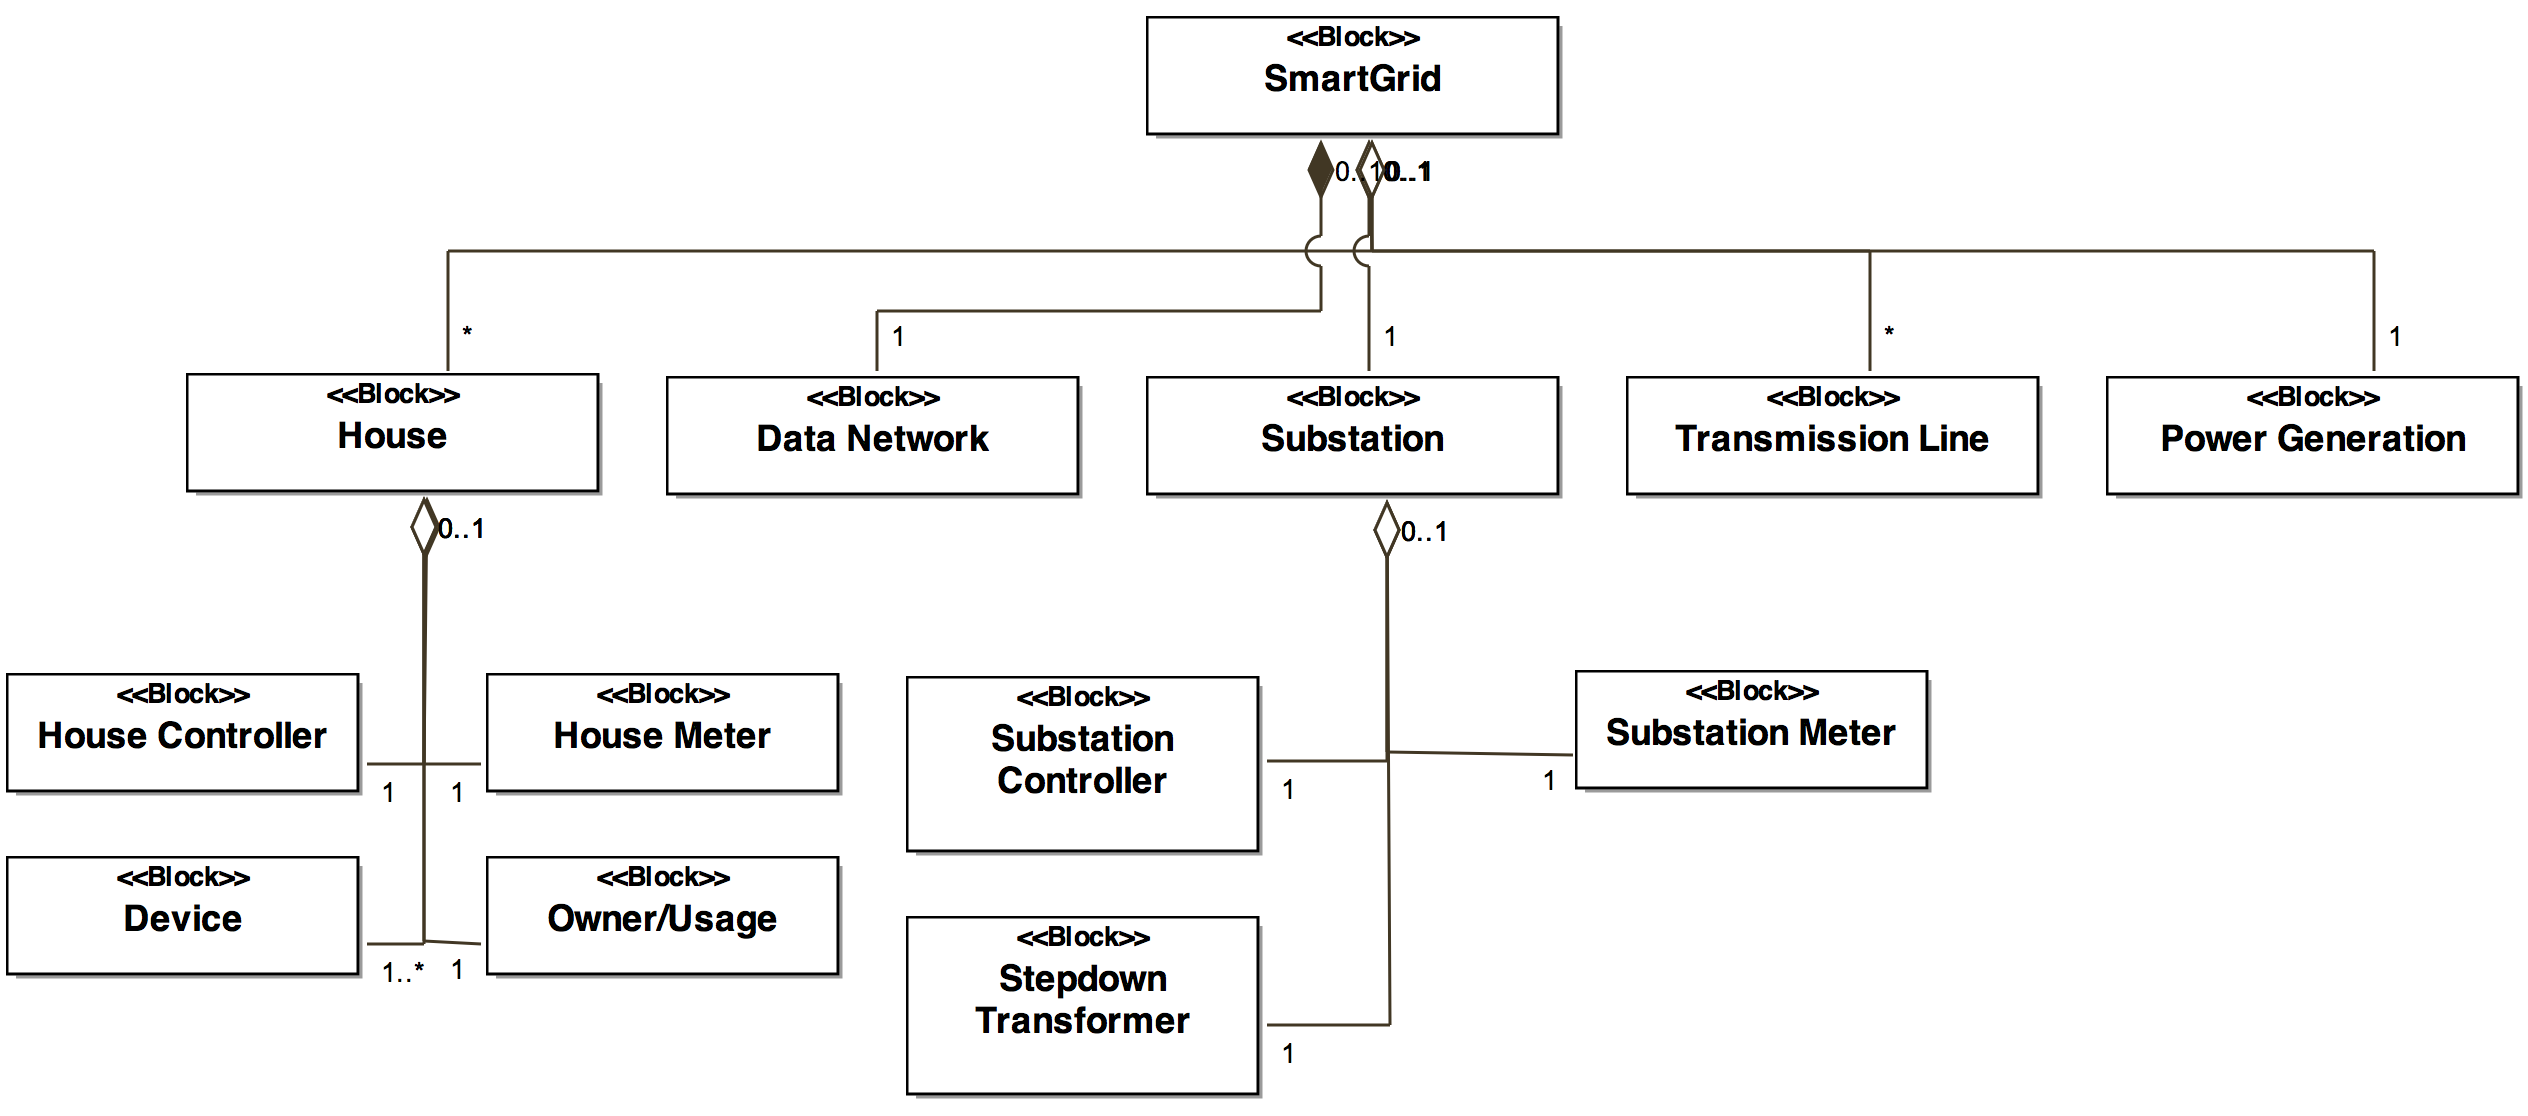
\includegraphics[width=1\textwidth]{figures/BDDSmartGrid}
\caption{Block Definition Diagram of Smart Grid}
\label{fig:bdd}
\end{figure}

An Internal Block Diagram (IBD) of the Smart Grid is given in Figure~\ref{fig:ibd}. The diagram shows there are two main connection types in the model, corresponding to the physical power connections and the cyber data connections. The model also shows the connections between the cyber and physical parts of the models -- currently modelled using data-type connections.

\begin{figure}
\centering
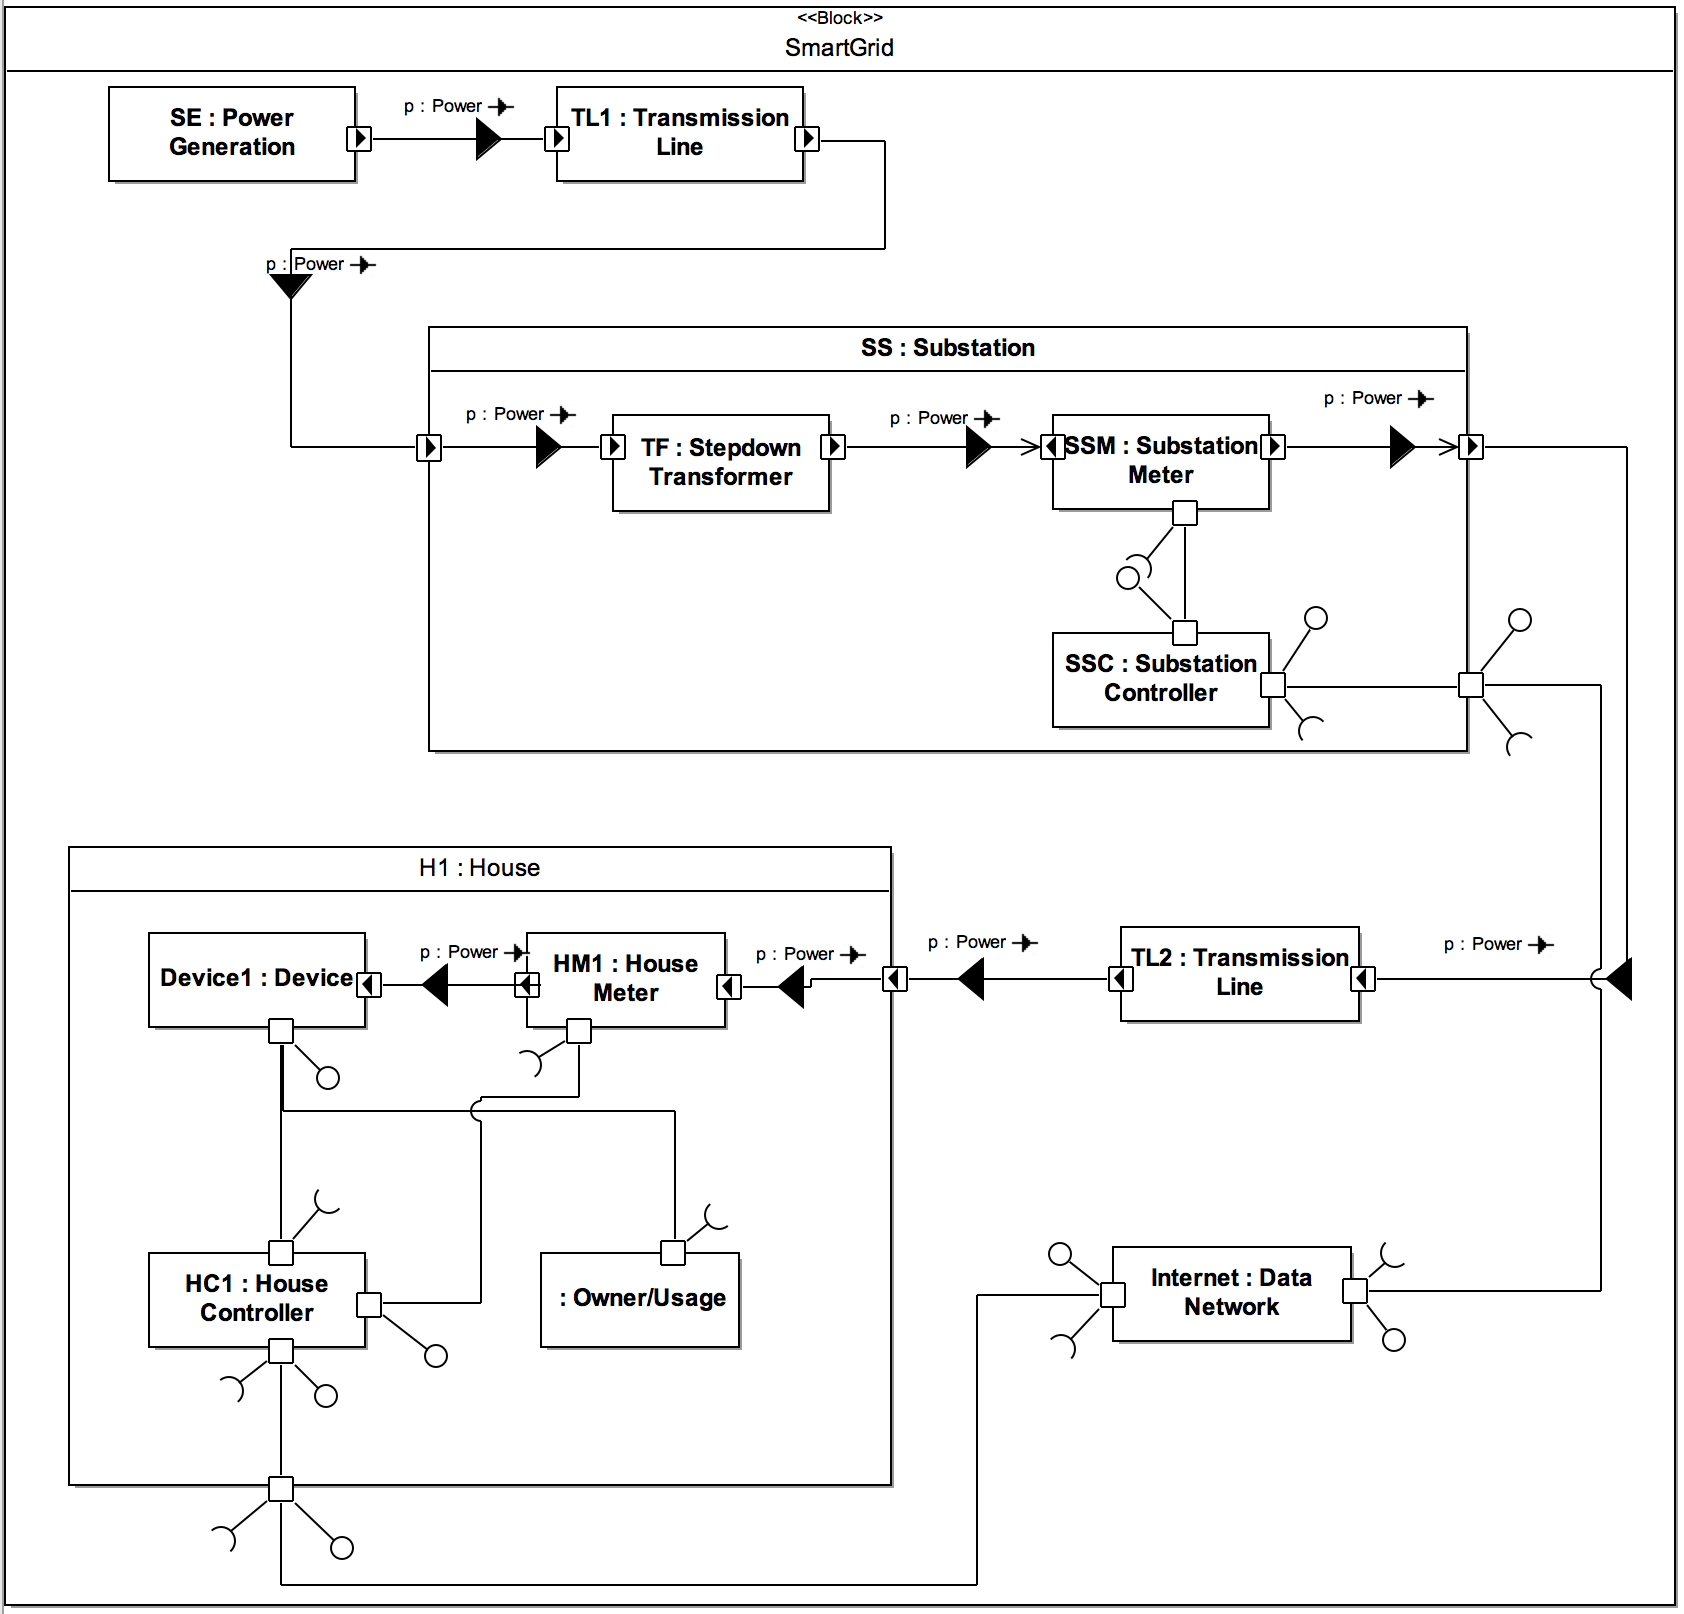
\includegraphics[width=0.85\textwidth]{figures/IBDSmartGrid}
\caption{Internal Block Diagram of Smart Grid}
\label{fig:ibd}
\end{figure}

The first type of connection ---the physical power connections--- show a flow of \textit{Power} from the Power Generation, through the Transmission Lines to the Houses, via the Substation. In the Substation, the Stepdown Transformer is connected to the Substation Meter. Similarly, in each House (only one is shown in the figure), the Power flows through the House Meter to each Device (again only one is shown for readability). The data connections exist between the Substation Controller and House Controllers. The Data Network is explicitly modelled and links the various controllers. Finally, there are links between the cyber controllers and the physical systems. In this model, the Substation Controller is connected to the Substation Meter, and the House Controller is linked to the House Meter and Devices.

\paragraph{Design Architectural Model}

% KGP: So actually we could update this to use CComponents to ``better reflect the holistic architecture''?

Looking at the holistic architecture defined in Figures~\ref{fig:bdd} and~\ref{fig:ibd} and moving towards a multi-model, we use the INTO-CPS SysML profile to define the architecture of the Smart Grid\ from the perspective of multi-model. This yields the ASD in Figure~\ref{fig:asd_mm}. This structure removes all subsystem structures such that each component is to be realised in a single FMU. Each element is defined as either a \emph{physical} or \emph{cyber} component, with the model type and platform identified.

\begin{figure}[htbp]
\centering
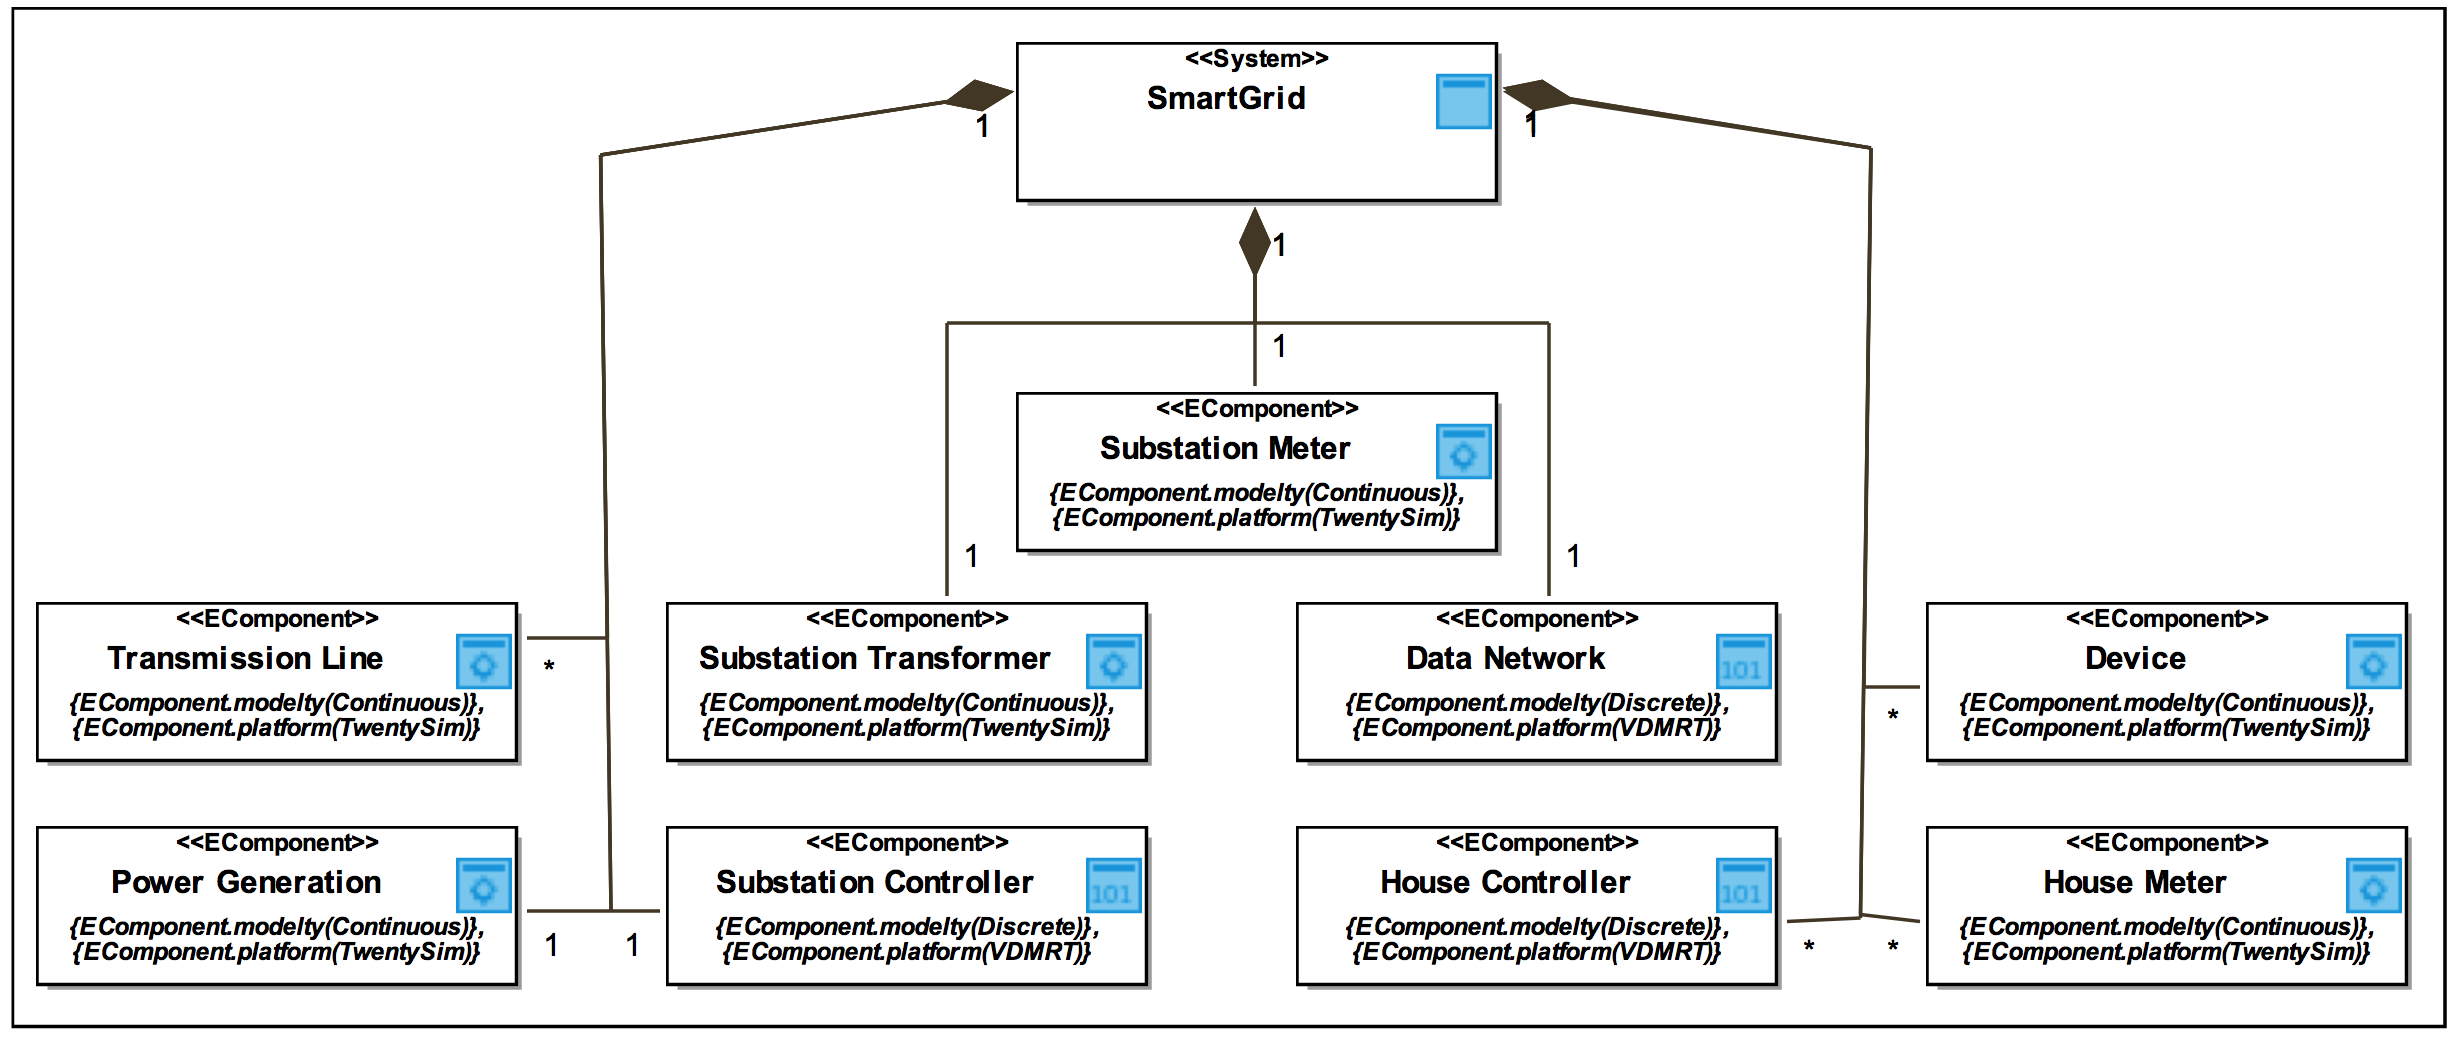
\includegraphics[width=0.9\textwidth]{figures/ASD_mm}
\caption{Architecture Structure Diagram for multi-model of Smart Grid}
\label{fig:asd_mm}
\end{figure}

The connections between the components are defined in the Connections Diagram (CD) in Figure~\ref{fig:cd_mm}. The interface between subsystems is defined as the interaction points between cyber and physical components (FMUs).

\begin{figure}
\centering
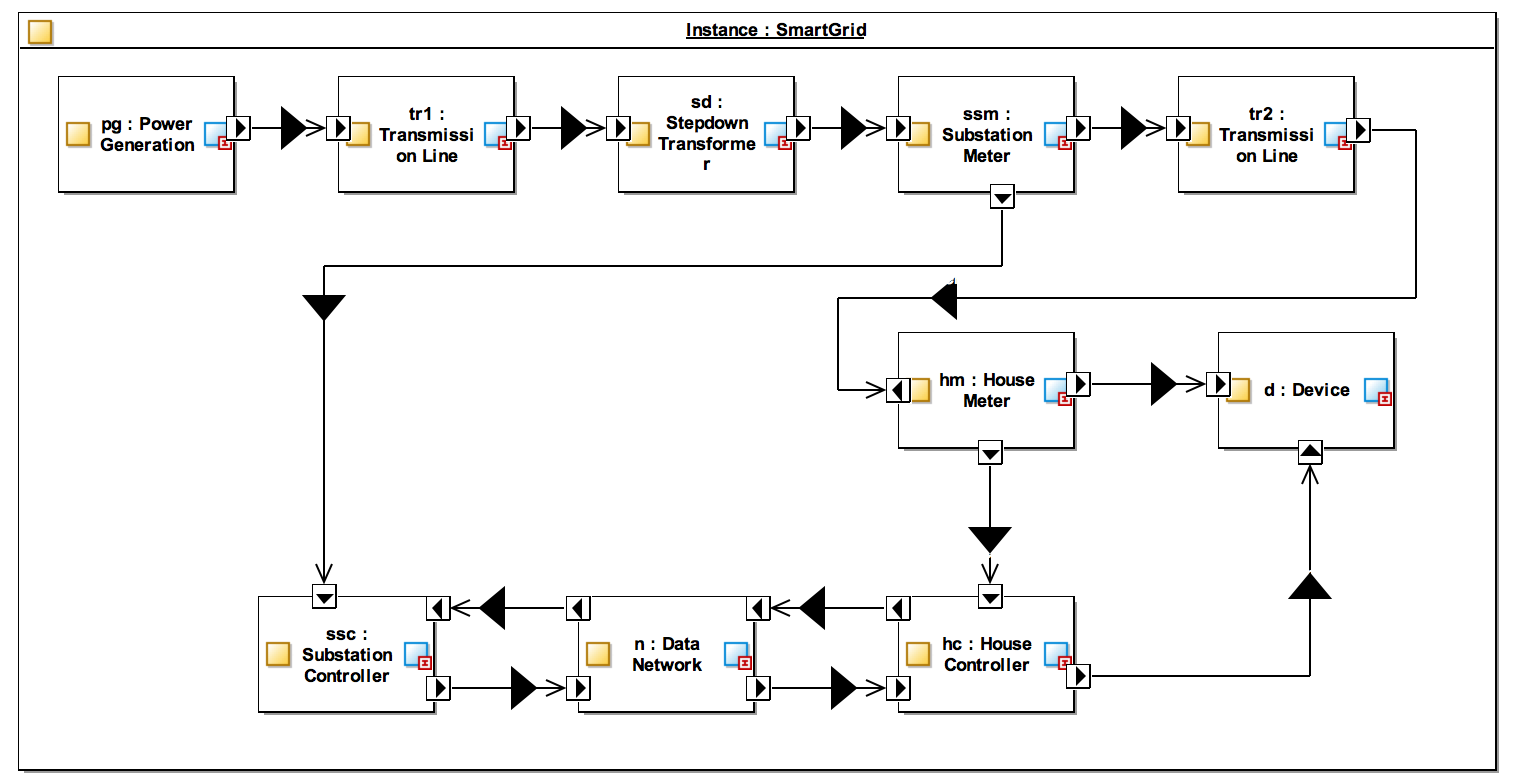
\includegraphics[width=1\textwidth]{figures/CD_mm}
\caption{Connections Diagram for multi-model of Smart Grid}
\label{fig:cd_mm}
\end{figure}

\paragraph{Discussion}

Contrasting the architectures shown in the initial model (Figures~\ref{fig:bdd} and~\ref{fig:ibd}) to that in the multi-model (Figures~\ref{fig:asd_mm} and~\ref{fig:cd_mm}), whilst the same base components are present in both, some of the intuitive domain-specific structures are lost when moving to a multi-model. For example, it is now not clear where the \emph{substation} or \emph{house} elements are in the multi-model.

An important issue here is in the reason behind producing different architectural models. Using SysML diagrams in a \emph{holistic} approach, a CPS engineer describes the model using a structure natural to the application domain. As such, the \emph{reason} for modelling is not in the ultimate analysis to perform, but to define and understand the structure and behaviour of a system. In contrast, the \emph{design} approach is necessary to configure INTO-CPS multi-models from SysML.

Figure~\ref{fig:sysml_mm} presents an overview of the relationships between the different types of models. The figure shows that the `real' system may be modelled in different forms: the holistic and design architectures and the multi-model.

\begin{figure}
\centering
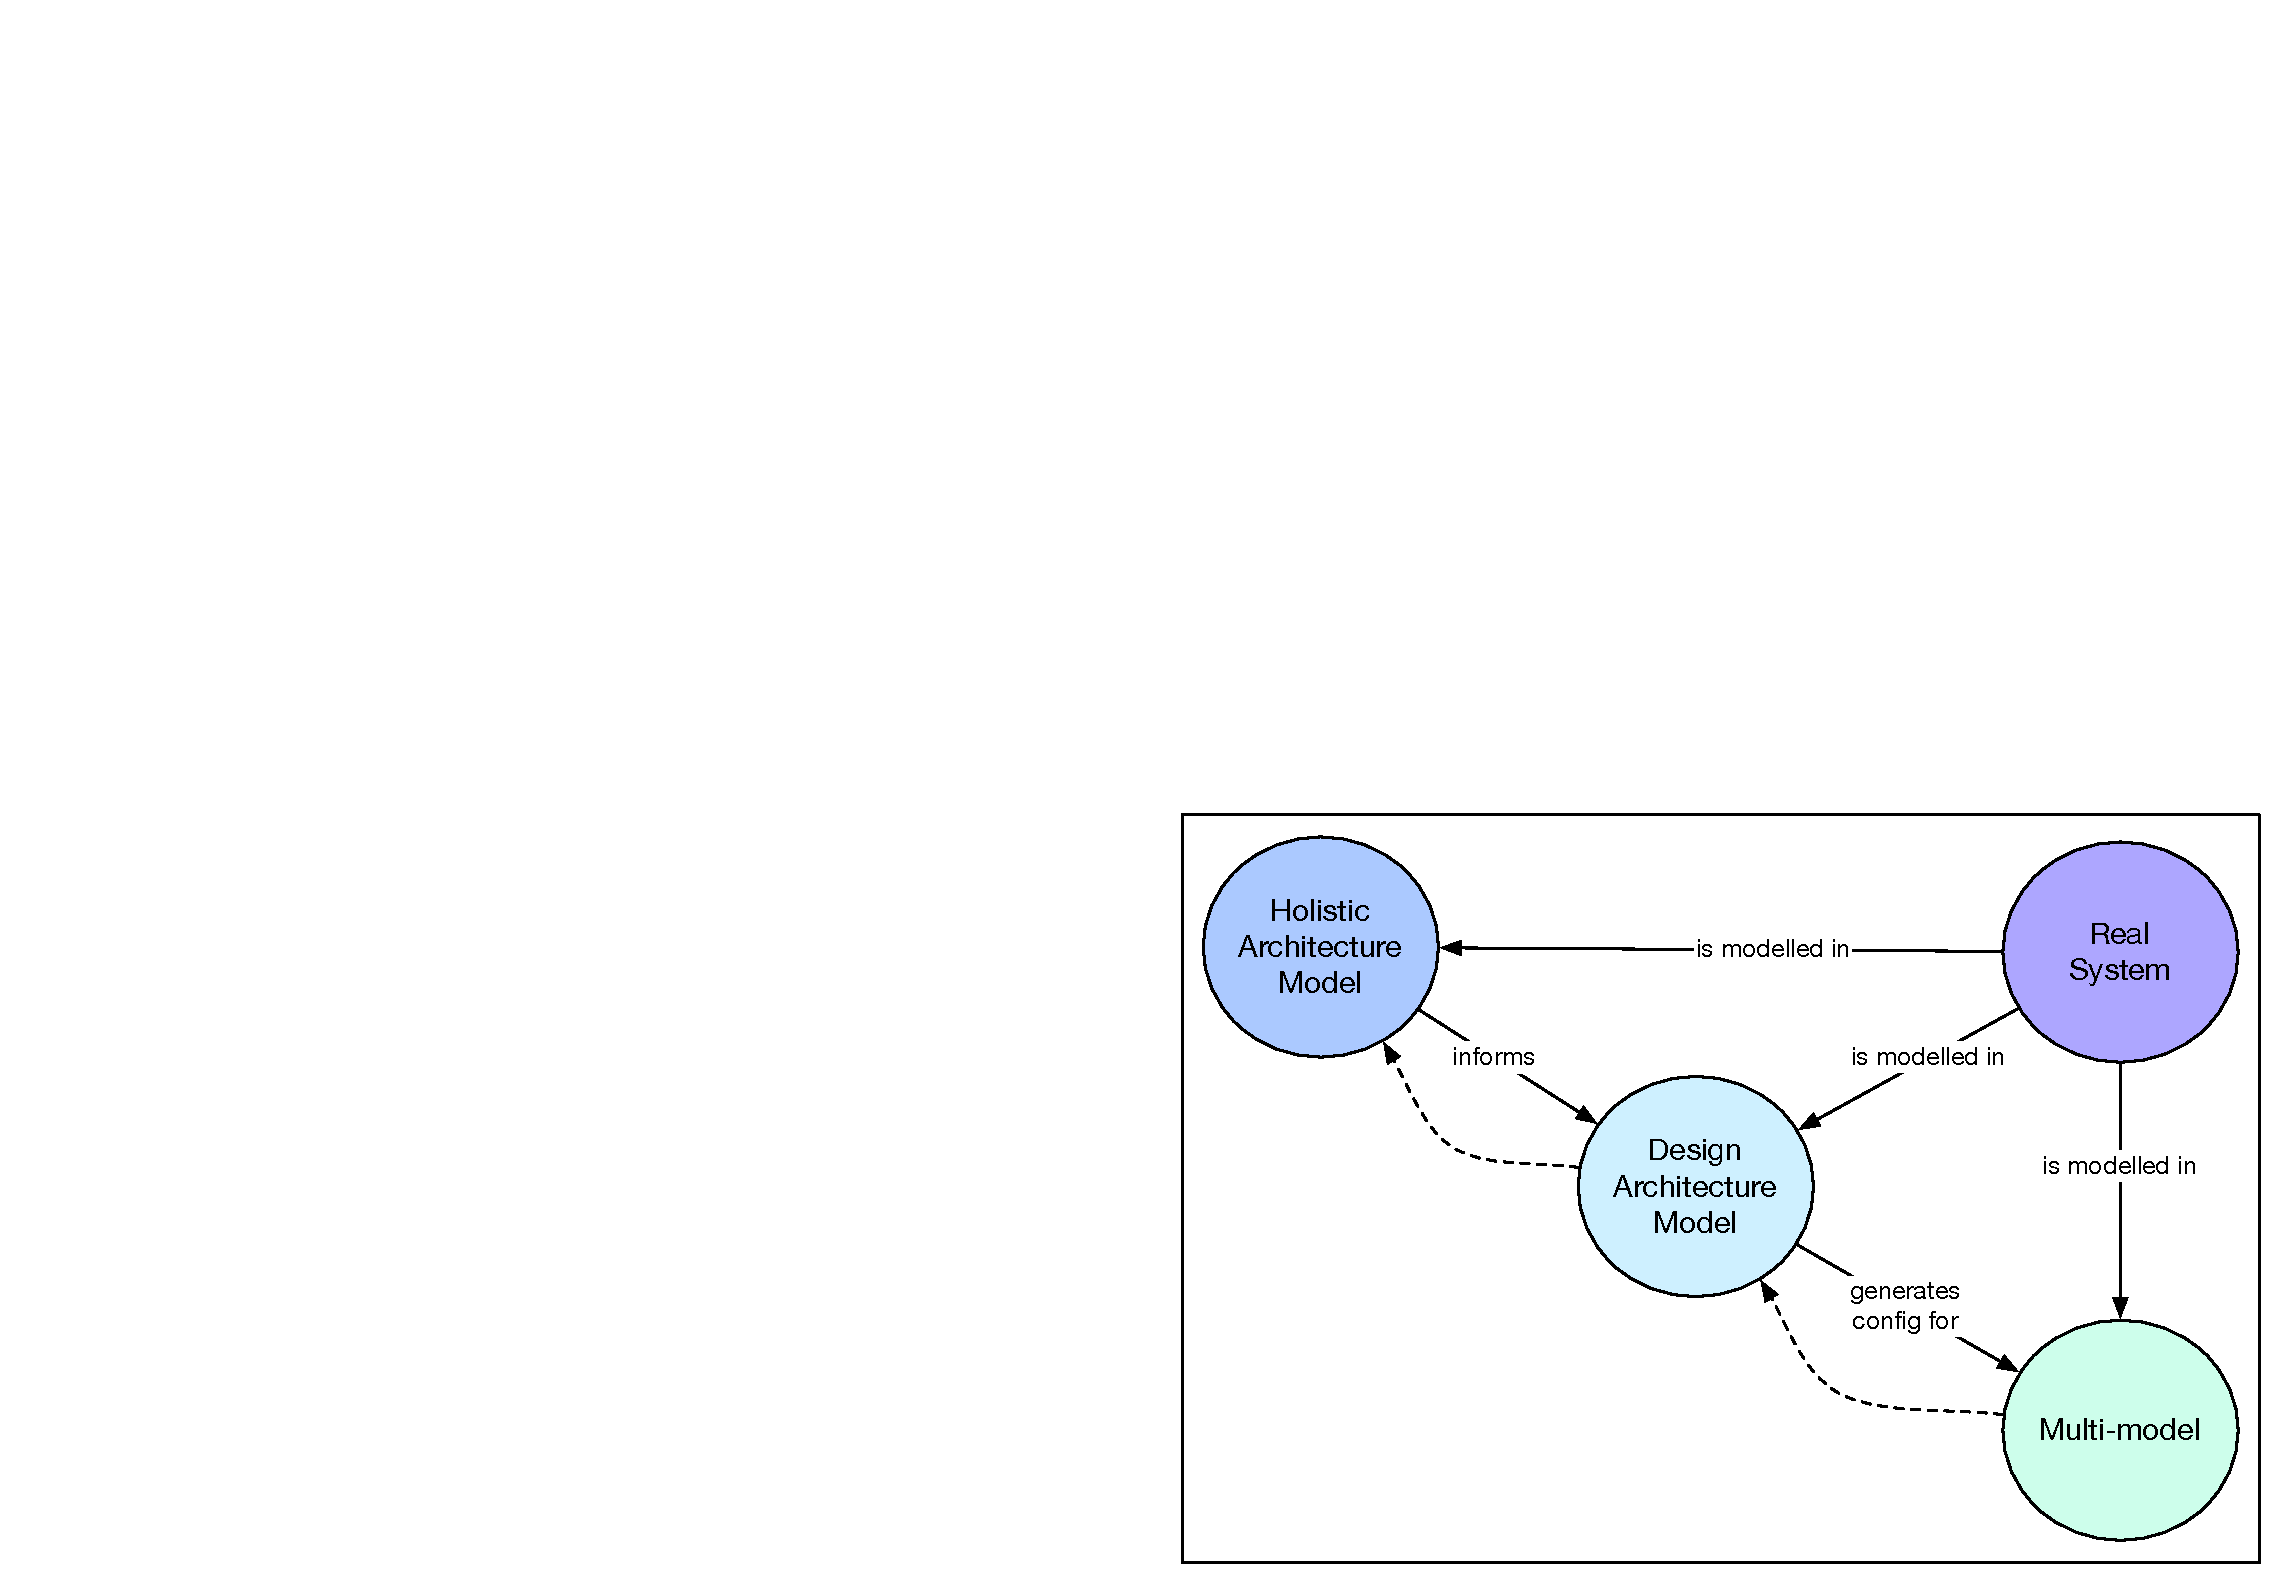
\includegraphics[width=0.7\textwidth]{figures/sysml_for_mm}
\caption{Relating holistic and design architectures}
\label{fig:sysml_mm}
\end{figure}

As illustrated in the figure, one approach can inform another. In some cases this may be a natural process; for example in the Smart Grid\ example, isolating each of the lowest level components in Figure~\ref{fig:bdd} to be individual FMUs in a multi-model is an evolution which will likely result in a feasible model. By creating a domain-specific holistic architecture first, then transforming these models into a design architecture for multi-modelling, design teams will likely gain the most benefit.


\subsubsection{Representing Non-Design Elements in SysML}
\label{sec:sysml:non-design}

Using the INTO-CPS tool chain, we generate co-simulation configurations using an architectural model defined with the INTO-SysML profile. This model defines the structure of a system in terms of the composition of its components and their connections. There are however circumstances where elements in the multi-model are not part of the design of the final system, for example where an FMU is used purely for visualisation. This FMU must be connected to the system components, however is not itself a system component. This is also true when considering the environment of the system.

Here we present a small example of the use of these extensions, using a simple robot example (based on the line-following robot pilot study, see Deliverable D3.6~\cite{INTOCPSD3.6}) to illustrate the use of \texttt{<<CComponent>>}s and the \emph{kind} of components (\emph{cyber}, \emph{physical}, \emph{environment}, \emph{visualisation}) described in Section~\ref{sec:sysml:intocps:asd} above.

The architecture structure diagram in Figure~\ref{fig:example_asd} shows: a \emph{System\_Env} block, an \texttt{<<EComponent>>} defined as an \texttt{Environment} FMU; a \emph{3D\_View} block an \texttt{<<EComponent>>}, defined as an \texttt{Visualisation} FMU; and an \emph{Example\_Robot} block, an \texttt{<<EComponent>>} defined as an \texttt{composition} of two FMUs.

\begin{figure}
\centering
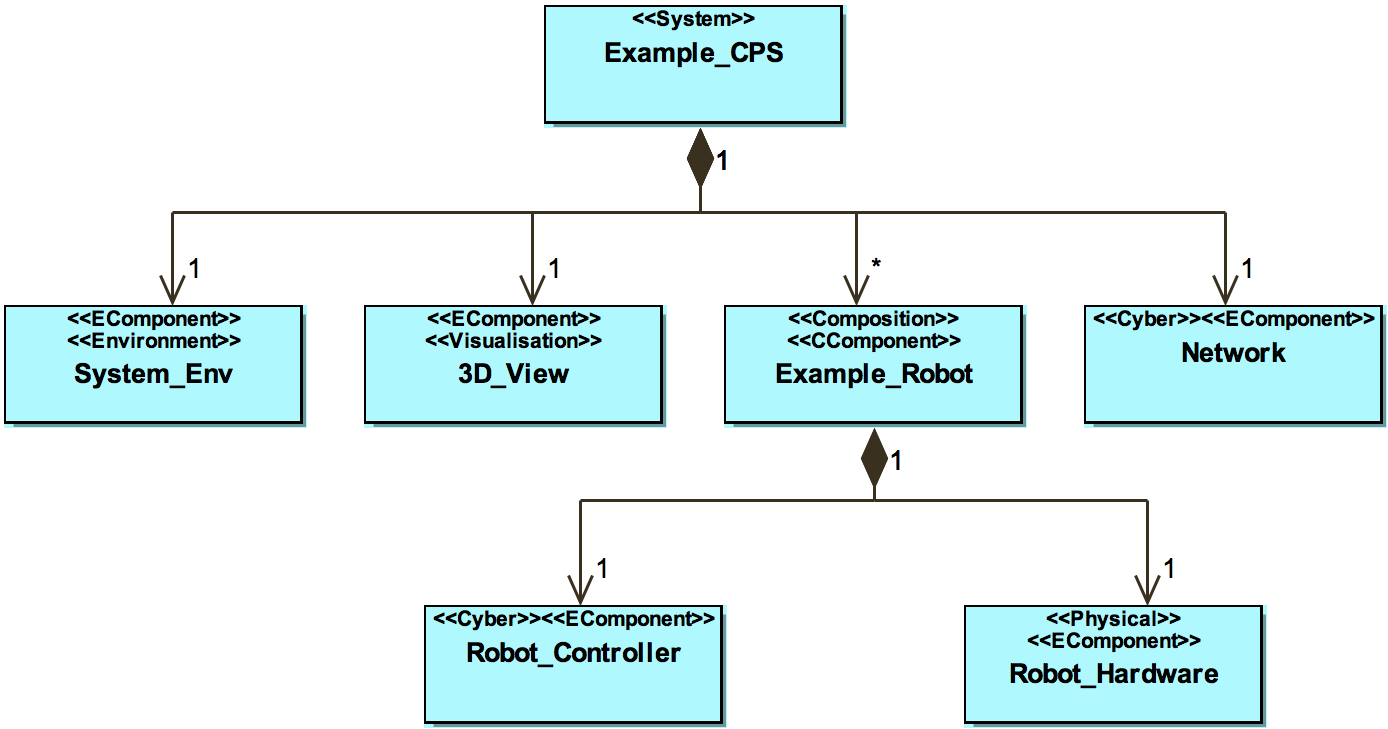
\includegraphics[width=0.8\textwidth]{figures/E_Blocks_ext_asd}
\caption{Example Architecture Structure Diagram of robot system}
\label{fig:example_asd}
\end{figure}

The example has two connection diagrams. The first is shown in Figure~\ref{fig:example_cd}, it contains only those connections with respect to the system and its constituent components . This diagram shows a block instance \emph{cps1} containing the environment (\emph{e}) and the example robot (\emph{r}) which  contains two the controller and hardware components.

The second is shown in Figure~\ref{fig:example_cd2}, it depicts the use of the block instance \emph{3D} of type \emph{3D\_View}. In this diagram, we show additional ports of the original block instances to output internal model details and connect these to the \emph{3D} instance. The diagram includes the system connectors as shown in Figure~\ref{fig:example_cd}.

\begin{figure}
\centering
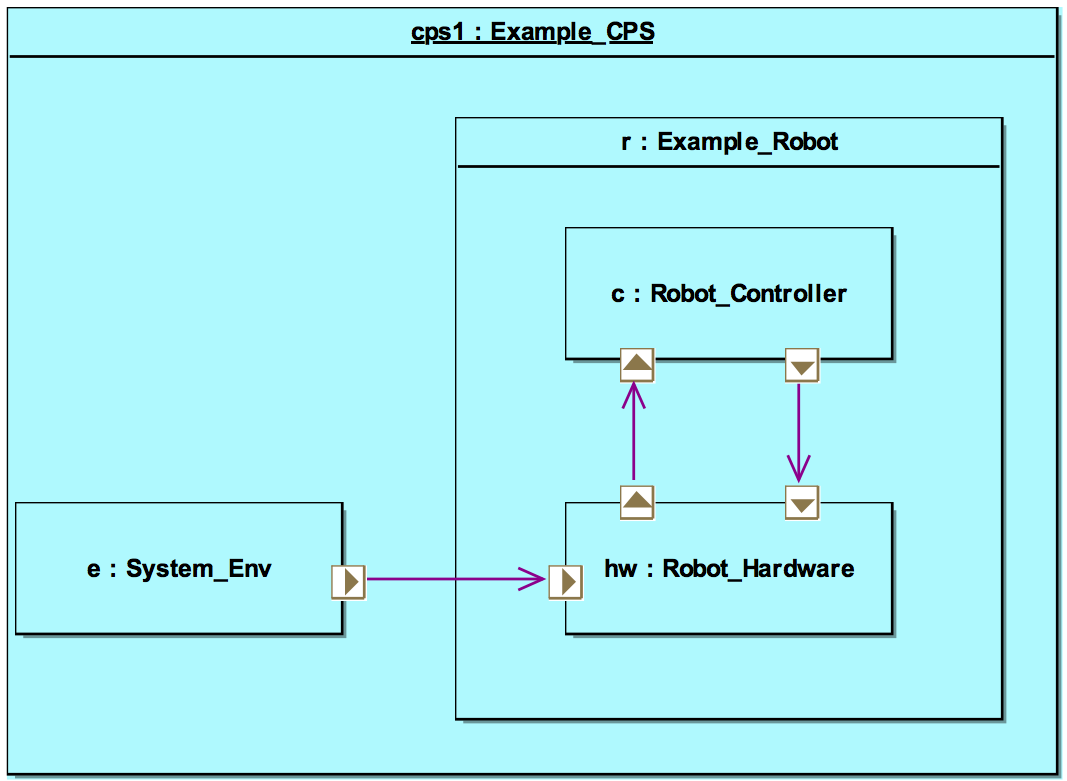
\includegraphics[width=0.6\textwidth]{figures/E_Blocks_ext_cd}
\caption{Connections Diagram for robot showing only system and environment connectors}
\label{fig:example_cd}
\end{figure}

\begin{figure}
\centering
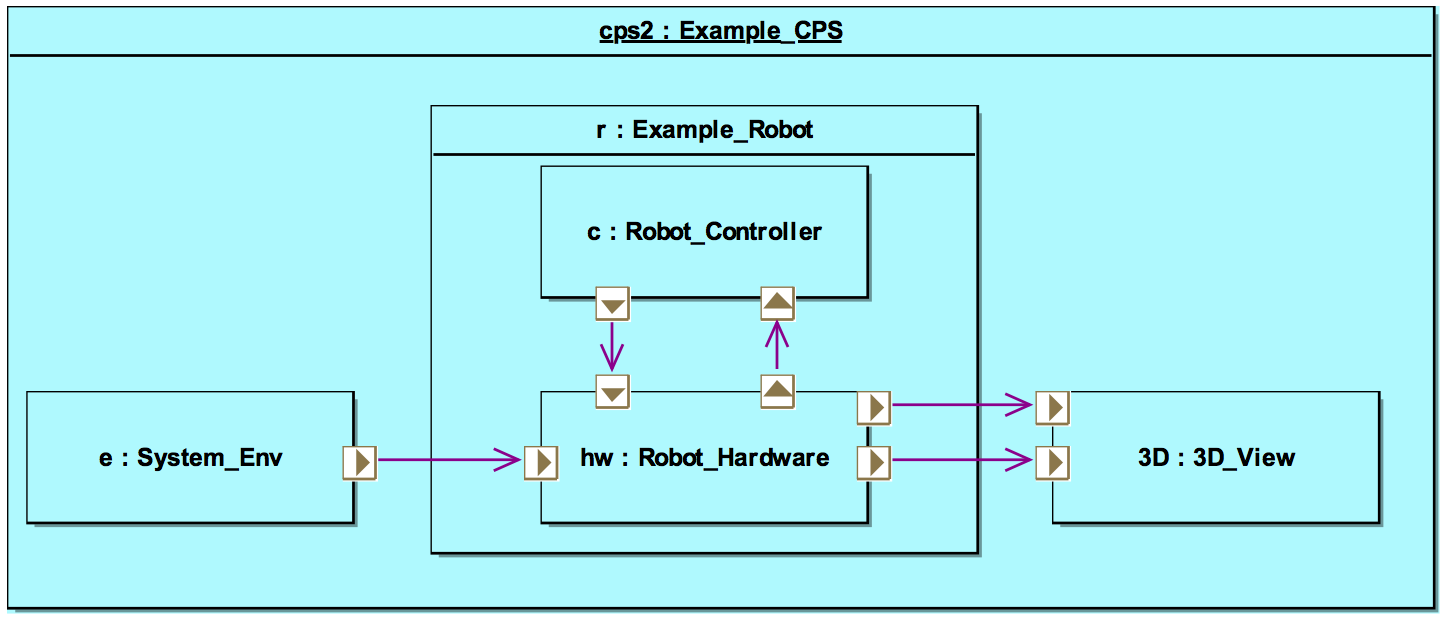
\includegraphics[width=0.9\textwidth]{figures/E_Blocks_ext_cd2}
\caption{Connections Diagram for the robot system showing the system \textit{and} visualisation components}
\label{fig:example_cd2}
\end{figure}



\paragraph{Initial Multi-Modelling using a Discrete-Event Notation: VDM}
\label{sec:method:defirst}

In this section we provide guidance on producing initial multi-models from architectural descriptions produced using the INTO-CPS SysML profile. We focus on using discrete-event (DE) models to produce initial, abstract FMUs that allow integration testing through co-simulation before detailed modelling work is complete. This is called a ``DE-first'' approach~\cite{Fitzgerald&13b,Fitzgerald&13a}. We describe the use of VDM and the Overture tool, with FMI export plug-in installed, for this approach. The principles outlined in this section can be applied in other modelling tools. This approach can work with or without the SysML profile.

%In future, these guidelines will be expanded to include how and when to continuous-time (CT) formalisms in initial modelling.

%\section{Context}
\subsection{The DE-first Approach}

\begin{figure}[p]
\centering
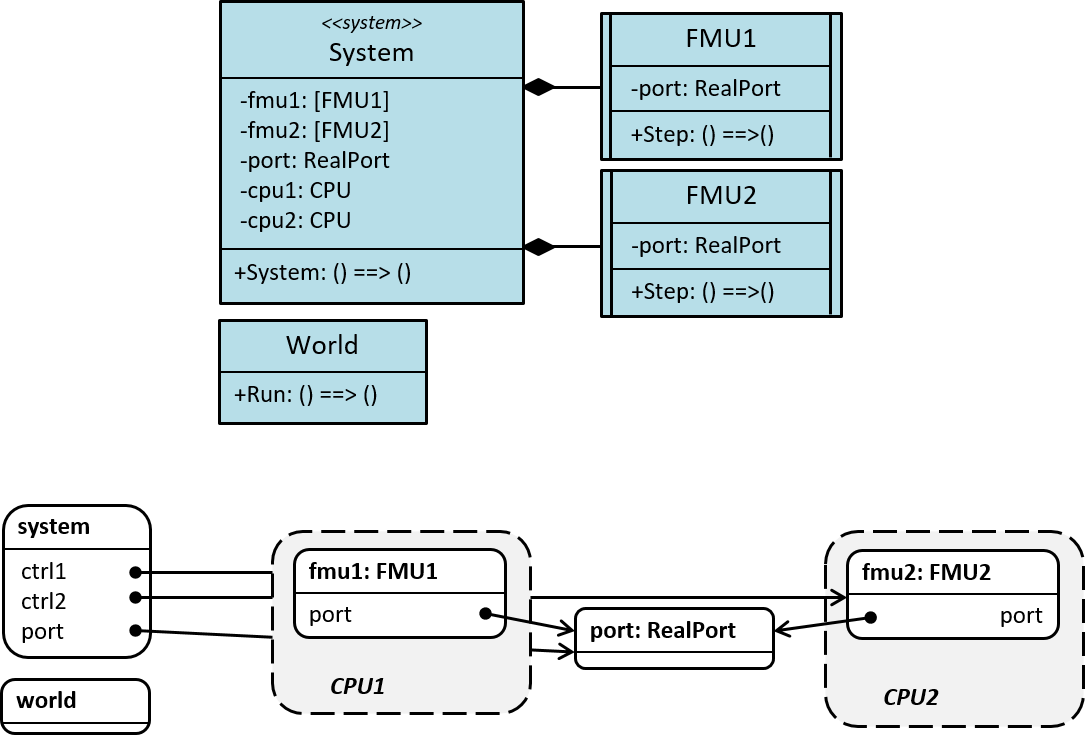
\includegraphics[scale=0.47]{figures/defirst_class}
\caption{Class diagram showing two simplified FMU classes created within a single VDM-RT project, and an object diagram showing them being instantiated as a test.}
\label{fig:defist_class}
\end{figure}

\begin{figure}[p]
\centering
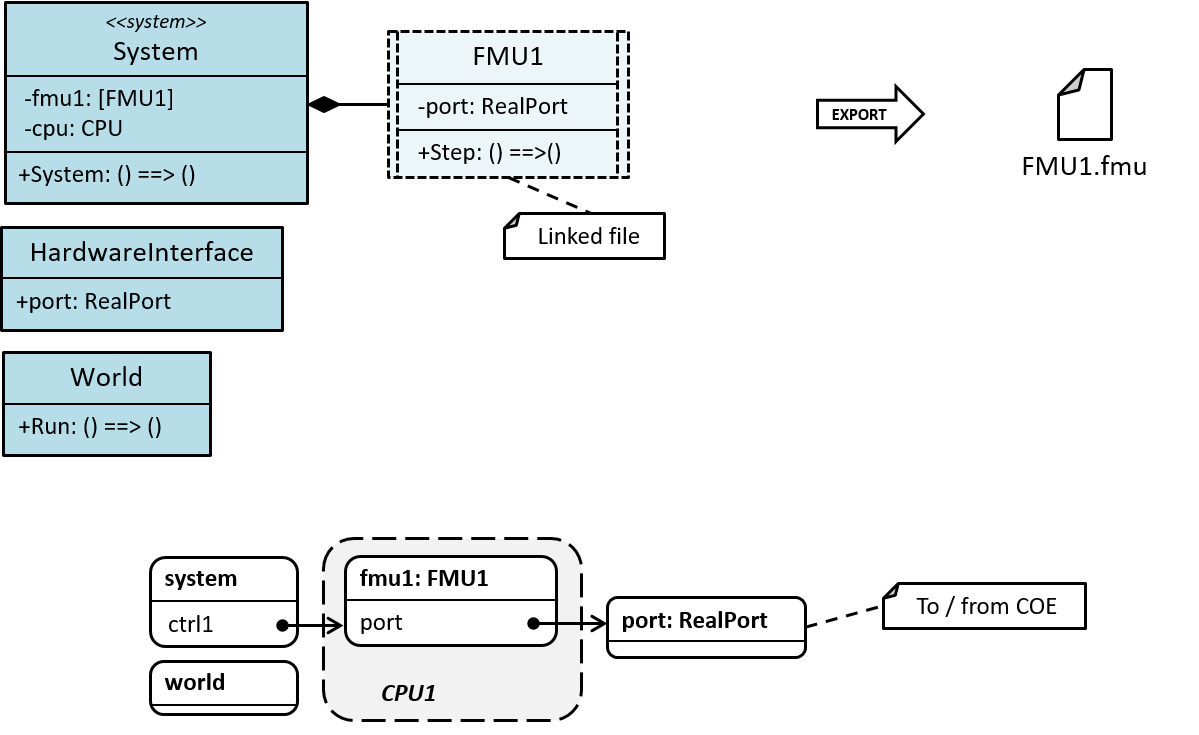
\includegraphics[scale=0.47]{figures/defirst_fmu1}
\caption{Class and object diagrams showing a linked class within its own project for FMU creation.}
\label{fig:defirst_fmus}
\end{figure}

After carrying out requirements engineering (RE), as described in Chapter~\ref{sec:reqeng}, and design architectural modelling in SysML, as described in Chapter~\ref{sec:sysml}, the engineering team should have the following artifacts available:

\begin{itemize}[noitemsep]
\item One or more Architecture Structure Diagrams (ASDs) defining the composition of\\ \texttt{<<EComponent>>}s (to be realised as \texttt{<<Cyber>>} or \texttt{<<Physical>>} FMUs) that will form the multi-model.
\item Model descriptions exported for each \texttt{<<EComponent>>}.
\item One or more Connections Diagrams (CDs) that will be used to configure a multi-model.
\end{itemize}

The next step is to generate a multi-model configuration in the INTO-CPS Application and populate it with FMUs, then run a first co-simulation. This however requires the source models for each FMU to be ready. If they already exist this is easy, however they may not exist if this is a new design. In order to generate these models, the model descriptions for each \texttt{<<EComponent>>} can be passed to relevant engineering teams to build the models, then FMUs can be passed back to be integrated.

It can be useful however to create and test simple, abstract FMUs first (or in parallel), then replace these with higher-fidelity FMUs as the models become available. This allows the composition of the multi-model to be checked early, and these simple FMUs can be reused for regression testing. This approach also mitigates the problem of modelling teams working at different rates.

Where these simple FMUs are built within the DE formalism (such as VDM), this is called a \emph{DE-first} approach. This approach is particularly appropriate where complex DE control behaviours ---such as supervisory control or modal behaviours--- are identified as a priority or where the experience of the modelling team is primarily in the DE domain~\cite{Fitzgerald&14c}.

Guidance on how to produce DE approximations for use in multi-modelling, and in particular approximations of CT behaviour, can be found in material describing the Crescendo baseline technology~\cite{Fitzgerald&13a}, which is also available via the Crescendo website\footnote{See \url{http://crescendotool.org/documentation/}}.

\subsubsection{DE-first within INTO-CPS}

Given an architectural structure diagram, connections diagram and model descriptions for each \texttt{<<EComponent>>}, the suggested approach is to begin by building a single VDM-RT project in Overture with the following elements:

\begin{itemize}[noitemsep]
\item A class for each \texttt{<<EComponent>>} representing an FMU. Each class should define port-type instance variables (i.e. of type \texttt{IntPort}, \texttt{RealPort}, \texttt{BoolPort}, or \texttt{StringPort}) corresponding to the model description and a constructor to take these ports as parameters. Each FMU class should also define a thread that calls a \texttt{Step} operation, which should implement some basic, abstract behaviour for the FMU.
\item A \texttt{system} class that instantiates port and FMU objects based on the connections diagram. Ports should be passed to constructor of each FMU object. Each FMU object should be deployed on its own CPU.
\item A \texttt{World} class that starts the thread of each FMU objects.
\end{itemize}

Class and object diagrams giving an example of the above is shown in Figure~\ref{fig:defist_class}. In this example, there are two \texttt{<<EComponent>>}s (called \emph{FMU1} and \emph{FMU2}) joined by a single connection of type real. Such a model can be simulated within Overture to test the behaviour of the FMUs. This approach can be combined with the guidance in Chapter~\ref{sec:networks} to analyse more complicated networked behaviour. Once the behaviour of the FMU classes has been tested, actual FMUs can be produced and integrated into a first multi-model by following the guidance below.

\subsubsection{FMU Creation}

The steps outlined below assume a knowledge of FMU export in Overture, which can be found in the User Manual, Deliverable D4.3a~\cite{INTOCPSD4.3a}, in Section 5.1. To generate FMUs, a project must be created for each \texttt{<<EComponent>>} with:

\begin{itemize}[noitemsep]
\item One of the FMU classes from the main project.
\item A \texttt{HardwareInterface} class that defines the ports and annotations required by the Overture FMU export plug-in, reflecting those defined in the model description.
\item A \texttt{system} class that instantiates the FMU class and passes the port objects from the \texttt{HardwareInterface} class to its constructor.
\item A \texttt{World} class that starts the thread of the FMU class.
\end{itemize}

The above structure is shown in Figure~\ref{fig:defirst_fmus}. A skeleton project with a correctly annotated \texttt{HardwareInterface} class can be generated using the model description import feature of the Overture FMU plug-in. The FMU classes can be linked into the projects (rather than hard copies being made) from the main project, so that any changes made are reflected in both the main project and the individual FMU projects. These links can be created by using the \emph{Advanced} section of the \emph{New \textgreater\ Empty VDM-RT File} dialogue, using the \texttt{PROJECT-1-PARENT\_LOC} variable to refer to the workspace directory on the file system (as shown in Figure~\ref{fig:defirst_link}). Note that if the FMU classes need to share type definitions, these can be created in a class called \texttt{Types} in the main project, then this class can be linked into each of the FMU projects in the same way.

From these individual project, FMUs can be exported and co-simulated within the INTO-CPS tool. These FMUs can then be replaced as higher-fidelity versions become available, however they can be retained and used for regression and integration testing by using different multi-model configurations for each combination.

\begin{figure}
\centering
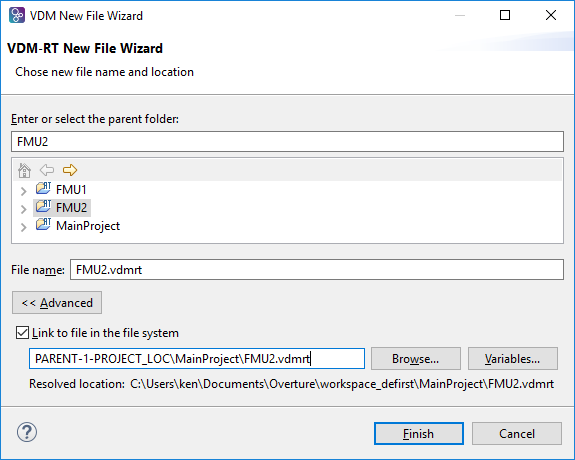
\includegraphics[scale=0.8]{figures/defirst_link}
\caption{Linking files in the \emph{New \textgreater\ Empty VDM-RT File} dialogue.}
\label{fig:defirst_link}
\end{figure}

\begin{figure}
\centering
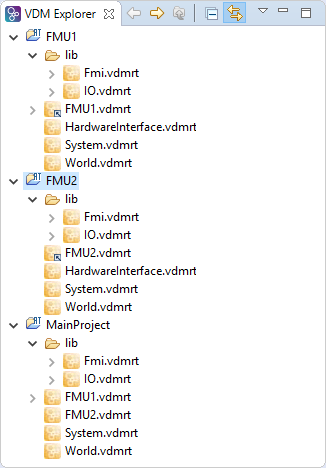
\includegraphics[scale=0.8]{figures/defirst_workspace}
\caption{Project structure of an Overture workspace showing a main project and two projects used for generating FMUs from linked class files.}
\label{fig:defirst_workspace}
\end{figure}

\subsection{Modelling Networks with VDM in Multi-models}
\label{sec:method:networks}
In this section, we address the problem of modelling networked controllers in multi-models, presenting a solution using VDM. When modelling and designing distributed controllers, it is necessary to model communications between controllers as well. While controller FMUs can be connected directly to each other through for co-simulation, this quickly becomes unwieldy due to the number of connections increasing exponentially. For example, consider the case of five controllers depicted in Figure~\ref{fig:bigraph}. In order to connect each controller together, 20 connections are needed (i.e.\ for a complete bidirected graph). Even with automatic generation of multi-model configurations, this is in general not a feasible solution.

\begin{figure}[hb]
\centering
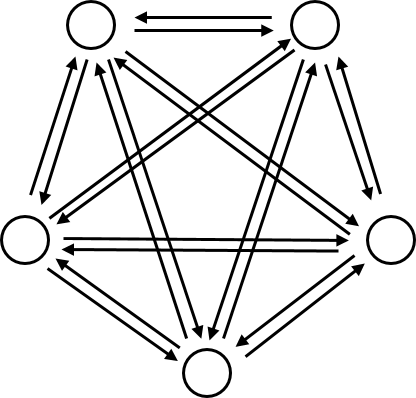
\includegraphics[scale=0.4]{figures/bigraph}
\caption{Topology of five controllers connected to each other}
\label{fig:bigraph}
\end{figure}

We suggest employing a pattern described initially as part of the Crescendo technology~\cite{Fitzgerald&14c}, in which a representation of an abstract communications medium called the `ether' is introduced. In the INTO-CPS setting, the ether is an FMU that is connected to each controller that handles message-passing between them. This reduces the number of connections needed, particularly for large numbers of controllers such as swarms. For five controllers, only 10 connections are needed, as shown in Figure~\ref{fig:bigraph2}.

\begin{figure}[hb]
\centering
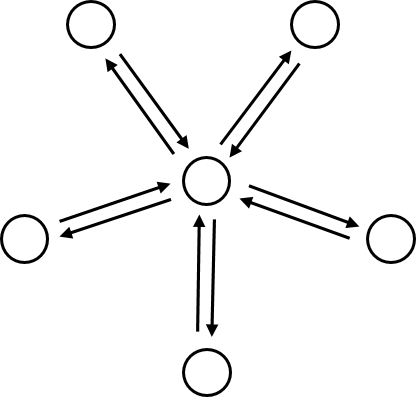
\includegraphics[scale=0.4]{figures/bigraph2}
\caption{Topology of five controllers connected via a shared medium}
\label{fig:bigraph2}
\end{figure}

In the remainder of this section, we describe how to pass messages between VDM FMUs using string types, how the ether class works, some of the consequences of using the ether pattern, and finally some extensions for providing quality of service (QoS) guarantees. %A class listing for a reference implementation of the \texttt{Ether} class is given in Appendix~\ref{app:ether}.
An example multi-model, called \emph{Case Study: Ether}, is available from the INTO-CPS Application. It is also described in the Examples Compendium, Deliverable D3.6~\cite{INTOCPSD3.6}.

\subsubsection{Representing VDM Values as Strings}

Connections between FMUs are typically numerical or Boolean types. This works well for modelling of discrete-time (DT) controllers and continuous-time (CT) physical models, however one of the advantages of VDM is the ability to represent more complex data types that better fit the abstractions of supervisory control. Therefore, in a multi-modelling setting, it is advantageous if VDM controllers can communicate with each other using data types that are not part of the FMI specification.

This can be achieved by passing strings between VDM FMUs (which are now supported by the Overture FMU export plug-in) and the \texttt{VDMUtil} standard library included in Overture, which can convert VDM types to their string representations and back again.

The \texttt{VDMUtil} library provides a (polymorphic) function called \texttt{val2seq\_of\_char}, that converts a VDM type to a string. It is necessary to tell the function what type to expect as a parameter in square brackets. For example, in the following listing, a 2-tuple is passed to the function, which will produce the output \texttt{"mk\_(2.4, 1.5)"}:

\begin{vdm}
VDMUtil`val2seq_of_char[real*real](mk_(2.4, 1.5))
\end{vdm}

The above can be used when sending messages as strings. In the model receiving message, the inverse function \texttt{seq\_of\_char2val} can be used. This function returns two values, a Boolean value indicating if the conversion was successful, and the value that was received:

\begin{vdm}
let mk_(b,v) = VDMUtil`val2seq_of_char[real*real](msg) in
  if b then ...
\end{vdm}

In the first few steps of co-simulation, empty or invalid strings are often passed as values, so it is necessary to check if the conversion was successful (as in the above listing) before using the value.

Note that currently (as of Overture 2.4.0), the \texttt{VDMUtil} library is called in the default scope, meaning that it does not know about custom types defined in the model. Therefore, it is recommended to pack values in a tuple (as in the above example) for message passing, then convert to and from any custom types in the sending and receiving models.

\subsubsection{Using the Ether FMU}

\begin{figure}
\centering
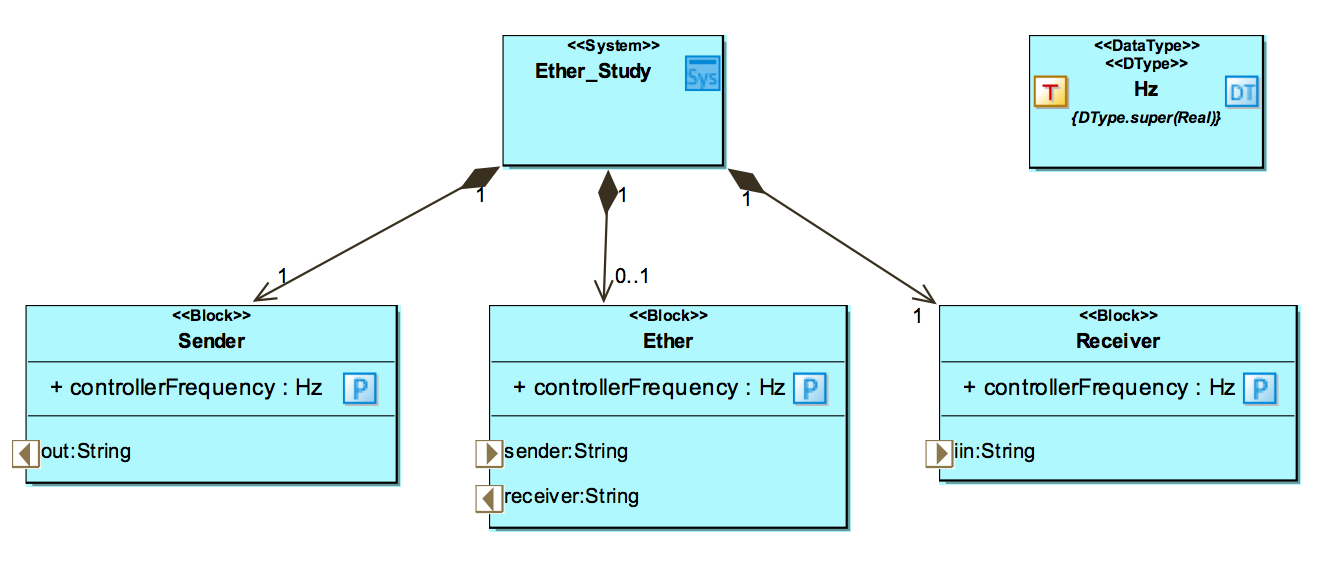
\includegraphics[scale=0.3]{figures/ether_asd}
\caption{\emph{Case Study: Ether} example}
\label{fig:ether_asd}
\end{figure}

By encoding VDM values as strings, it is possible to define a simple broadcast ether that receives message strings on its input channel(s) and sends them to its output channel(s). As a concrete example, we consider the \emph{Case Study: Ether} (see Deliverable D3.5~\cite{INTOCPSD3.5}), which contains a \texttt{Sender}, a \texttt{Receiver} and an \texttt{Ether}, as depicted in Figure~\ref{fig:ether_asd}. In this example, the three FMUs have the following roles:

\begin{description}[noitemsep]
  \item[Sender] Generates random 3-tuple messages of type \texttt{real * real * real}, encodes them as strings using the \texttt{VDMUtil} library and puts them on its output port.
  \item[Receiver] Receives strings on its input port and tries to convert them to single messages of type \texttt{real * real * real} or to a sequence of messages of type of type \texttt{seq of (real * real * real)}.
  \item[Ether] Has an input port and output port, each assigned a unique identifier, i.e. as a \texttt{map Id to StringPort}. It also has a mapping of input to output ports as a set of pairs: \texttt{set of (Id * Id)}. It has a list that holds messages for each output destination, because multiple messages might arrive for one destination. It gathers messages from each input and passes them to the outputs defined in the above mapping.
\end{description}

In this simple example, the sender and receiver are asymmetrical, but in more complicated examples controllers can be both senders and receivers by implementing both of the behaviours described above.

The \emph{Case Study: Ether} example contains two multi-models that allow the sender and receiver to be connected directly (connection diagram shown in Figure~\ref{fig:snd_rec}), or to be connected via the ether (connection diagram shown in Figure~\ref{fig:snd_ether_rec}). The description in the Examples Compendium, Deliverable D3.5~\cite{INTOCPSD3.5}, explains how to run the two different multi-models. This approach shows that the use of string ports and the \texttt{VDMUtil} library can be useful even without the ether for message passing between controllers in simple topologies.

For the sender, this connection is transparent, it does not care whether it is connected to the ether or not. For the receiver, in the direct connection it will receive single messages, whereas when receiving from the ether it will receive a list of messages (even for a single value). So the receiver is able to deduce when it is directly connected or connected via the ether. 



\begin{figure}
\centering
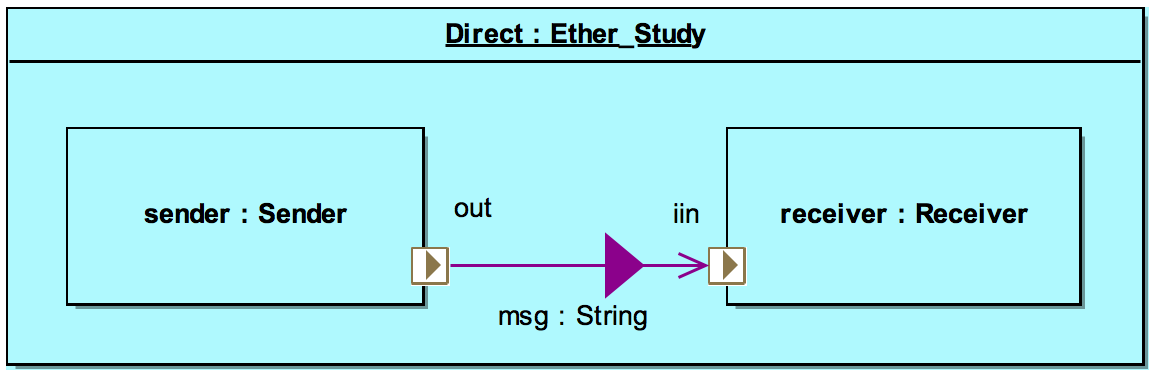
\includegraphics[scale=0.2]{figures/ether_cd_direct}
\caption{Connection diagram of the \emph{Direct} multi-model in the \emph{Case Study: Ether} example}
\label{fig:snd_rec}
\end{figure}

\begin{figure}
\centering
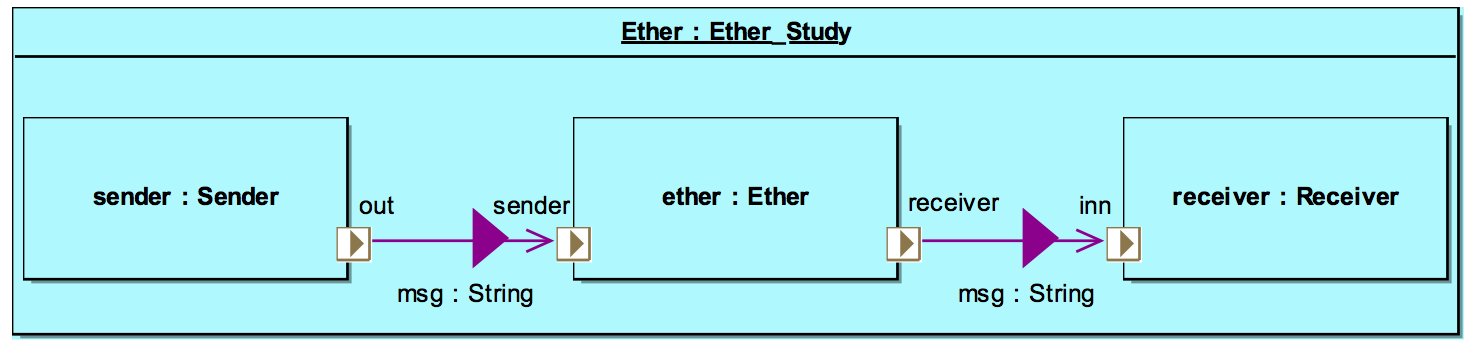
\includegraphics[scale=0.25]{figures/ether_cd_ether}
\caption{Connection diagram of the \emph{Ether} multi-model in the \emph{Case Study: Ether} example}
\label{fig:snd_ether_rec}
\end{figure}

The ether defined in this example is intended to be generic enough that it can be used in other case studies that need a simple broadcast ether without guarantees of delivery. To use it, you can:

\begin{enumerate}[noitemsep]
\item Import the \emph{Ether} model from the \emph{case-study\_ether/Models} directory into Overture;
\item Update the \texttt{HardwareInterface}\footnote{A class that provides annotated definitions of the ports for a VDM FMU.} class to provide input and/or output ports for all controllers that will be connected to the ether.
\item Update the \texttt{System} class to assign identifiers to all input and output ports; and
\item Update the set of identifier pairs that define connections.
\end{enumerate}

\subsubsection{Consequences of Using the Ether}

The ether as presented above %, and listed in Appendix~\ref{app:ether},
is fairly basic. In each update cycle, it passes values from its input variables to their respective output variables. This essentially replicates the shared variable style of direct FMU-FMU connections, which means that the relative update speeds of the FMUs may lead to the following:

\begin{description}[noitemsep]
  \item[Values may be delayed] The introduction of an intermediate FMU means that an extra update cycle is required to pass values from sender to ether and ether to receiver. This may delay messages unless the ether updates at least twice as fast as the receiver.
  \item[Values may not be read] If a value is not read by the receiver before it is changed, then that value is lost.
  \item[Values may be read more than once] If a value is not changed by the sender before the receiver updates, then the value is read twice. In the simple ether, the receiver cannot distinguish an old message from a new message with the same values.
\end{description}

In the Examples Compendium, Deliverable D3.5~\cite{INTOCPSD3.5}, the \emph{Case Study: Ether} example is described along with some suggested experiments to see the effects of the above examples by changing the controller frequency parameters of the sender, ether and receiver. In the final part of this section we outline ways to overcome such problems if it is necessary to guarantee that messages arrive and are read during a co-simulation.

\subsubsection{Modelling True Message Passing and Quality of Service}

The key to achieving a true message-passing is to overcome the problem of distinguishing old messages from new messages with the same values. This can be done by attaching a unique identifier to each message, which could be, for example, an identifier of the sender plus a message number:

\newpage
\begin{vdm}
instance variables

id: seq of char := "a";
seqn: nat1 := 1;

...

VDMUtil`val2seq_of_char[seq of char*real*real](
  mk_(id ^ [seqn], 2.4, 1.5));
seqn := seqn + 1
\end{vdm}

The advantage of assigning an identifier to each controller is that messages could also contain destination addresses, instead of the broadcast model presented above. In order to achieve these, some changes are needed to allow for acknowledging receipt of messages. Controllers should:

\begin{enumerate}[noitemsep]
\item Send a queue of messages on their output channel along with message identifiers of (recently received) messages;
\item Expect to receive a queue of messages along with message identifiers of successfully sent messages; and
\item Senders should remove messages from their output queue once their receipt has been acknowledged.
\end{enumerate}

The \texttt{Ether} class must be extended to:

\begin{enumerate}[noitemsep]
\item Inspect the message identifier (and destination if required) using \texttt{VDMUtil};
\item Pass message identifiers back to senders to acknowledge receipts; and
\item Listen for message identifiers from receivers to know when to remove messages from the queue.
\end{enumerate}

A dedicated channel for acknowledging messages could also be introduced, which would simplify the above. Therefore, each controller would have four connections to the ether: send and acknowledge, receive and acknowledge, as depicted in Figure~\ref{fig:ack}.

\begin{figure}
\centering
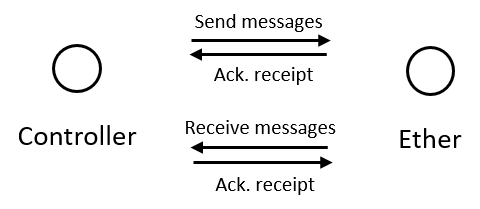
\includegraphics[scale=0.6]{figures/ack_channel}
\caption{Topology of controller to \emph{Ether} connection with dedicated channels for messages and acknowledgements}
\label{fig:ack}
\end{figure}

The advantages of guaranteed message delivery as described here are that realistic and faulty behaviour of the communication medium can be studied. An ether can be produced that provides poorer quality of service (delay, loss, repetition, reordering). These behaviours could be parameterised and explored using DSE (see Chapter~\ref{sec:dse}). By controlling for problems introduced by the nature of co-simulation, any reduction in performance of the multi-model can be attributed to the realistic behaviour introduced intentionally into the model of communications.


\subsection{Design Space Exploration}
\label{sec:method:dse}

In this section, we outline guidelines for  DSE over co-models of CPSs that: (a) support decision management by helping engineers to articulate clearly the parameters, objectives and metrics of a DSE analysis (Section~\ref{sec:dse-sysml}); and (b) enable the tuning of DSE methods for given domains and systems of interest (Section~\ref{sec:dse-algorithms}).
%
%
%\section{Experiment variables}
%
%\fbox{introduce parameters, architectures and scenarios and how they differ}
%
%

%
%\section{Ranking of designs}
%
%\fbox{methods for ranking and how they differ}
%


\subsubsection{Guidelines for Designing DSE in SysML}
\label{sec:dse-sysml}
\label{sec:dse-linefollow}

\paragraph{Rationale}

Designing DSE experiments can be complex and tied closely to the multi-model being analysed. The definitions guiding the DSE scripts should not just appear with no meaningful links to the any other artefacts in the \into\ Tool  chain. There are two main reasons for this, firstly there is no traceability back to the requirements from which we might understand why the various objectives (measures) were being evaluated or why they were included in the ranking definition.  Secondly, if DSE configurations are created manually for each new DSE experiment it is easy to imagine that the DSE analysis and ranking might not be consistent among the experiments.

Engineers need, therefore, to be able to model at an early stage of design how the experiments relate to the model architecture, and where possible trace from requirements to the analysis experiments. Here we describe the first step towards this vision: a SysML profile for modelling DSE experiments. The profile comprises five diagrams for defining \emph{parameters}, \emph{objectives} and \emph{rankings}.

We take the same approach to defining the SysML profile for DSE as that used to define the INTO-SysML profile.  A metamodel is defined (see Deliverable D3.2b~\cite{INTOCPSD3.2b}) and the collection of profile diagrams that implement this metamodel are defined in Deliverable D4.2c~\cite{INTOCPSD4.2c}.

In this section, we present an illustrative example of the use of the DSE-SysML profile -- from requirements engineering through defining parameters and objectives in the DSE-SysML profile to the final DSE JSON configuration files. We present result of the execution of DSE for the defined configuration.

As an example, we use the line follower robot pilot study. More details can be found in Deliverable D3.5~\cite{INTOCPSD3.5}.

\paragraph{Requirements}

We propose the use of a subset of the SoS-ACRE method detailed in Chapter~\ref{sec:reqeng} (as this section concentrates on the application of the DSE-SysML profile, we don't consider the full SoS-ACRE process). In the Requirements Definition View in Figure~\ref{fig:line_rdv}, the following five requirements are defined:

\begin{enumerate}
	\item The robot shall have a minimal cross track error
	\item The cross track error shall never exceed \textbf{X} mm
	%\item The robot shall maximise its potential range
	%\item The robot shall have a minimal range of \textbf{X} m
	\item The robot shall maximise its average speed
	\item The robot shall have a minimum average speed of \textbf{X} ms$^{-1}$
%	\item The robot shall maximise its operating time between battery charges
%	\item The robot shall have a minimum operating time of \textbf{X}s
	\item The robot sensor positions may be altered to achieve global goals
\end{enumerate}

\begin{figure}[htbp]
	\centering
	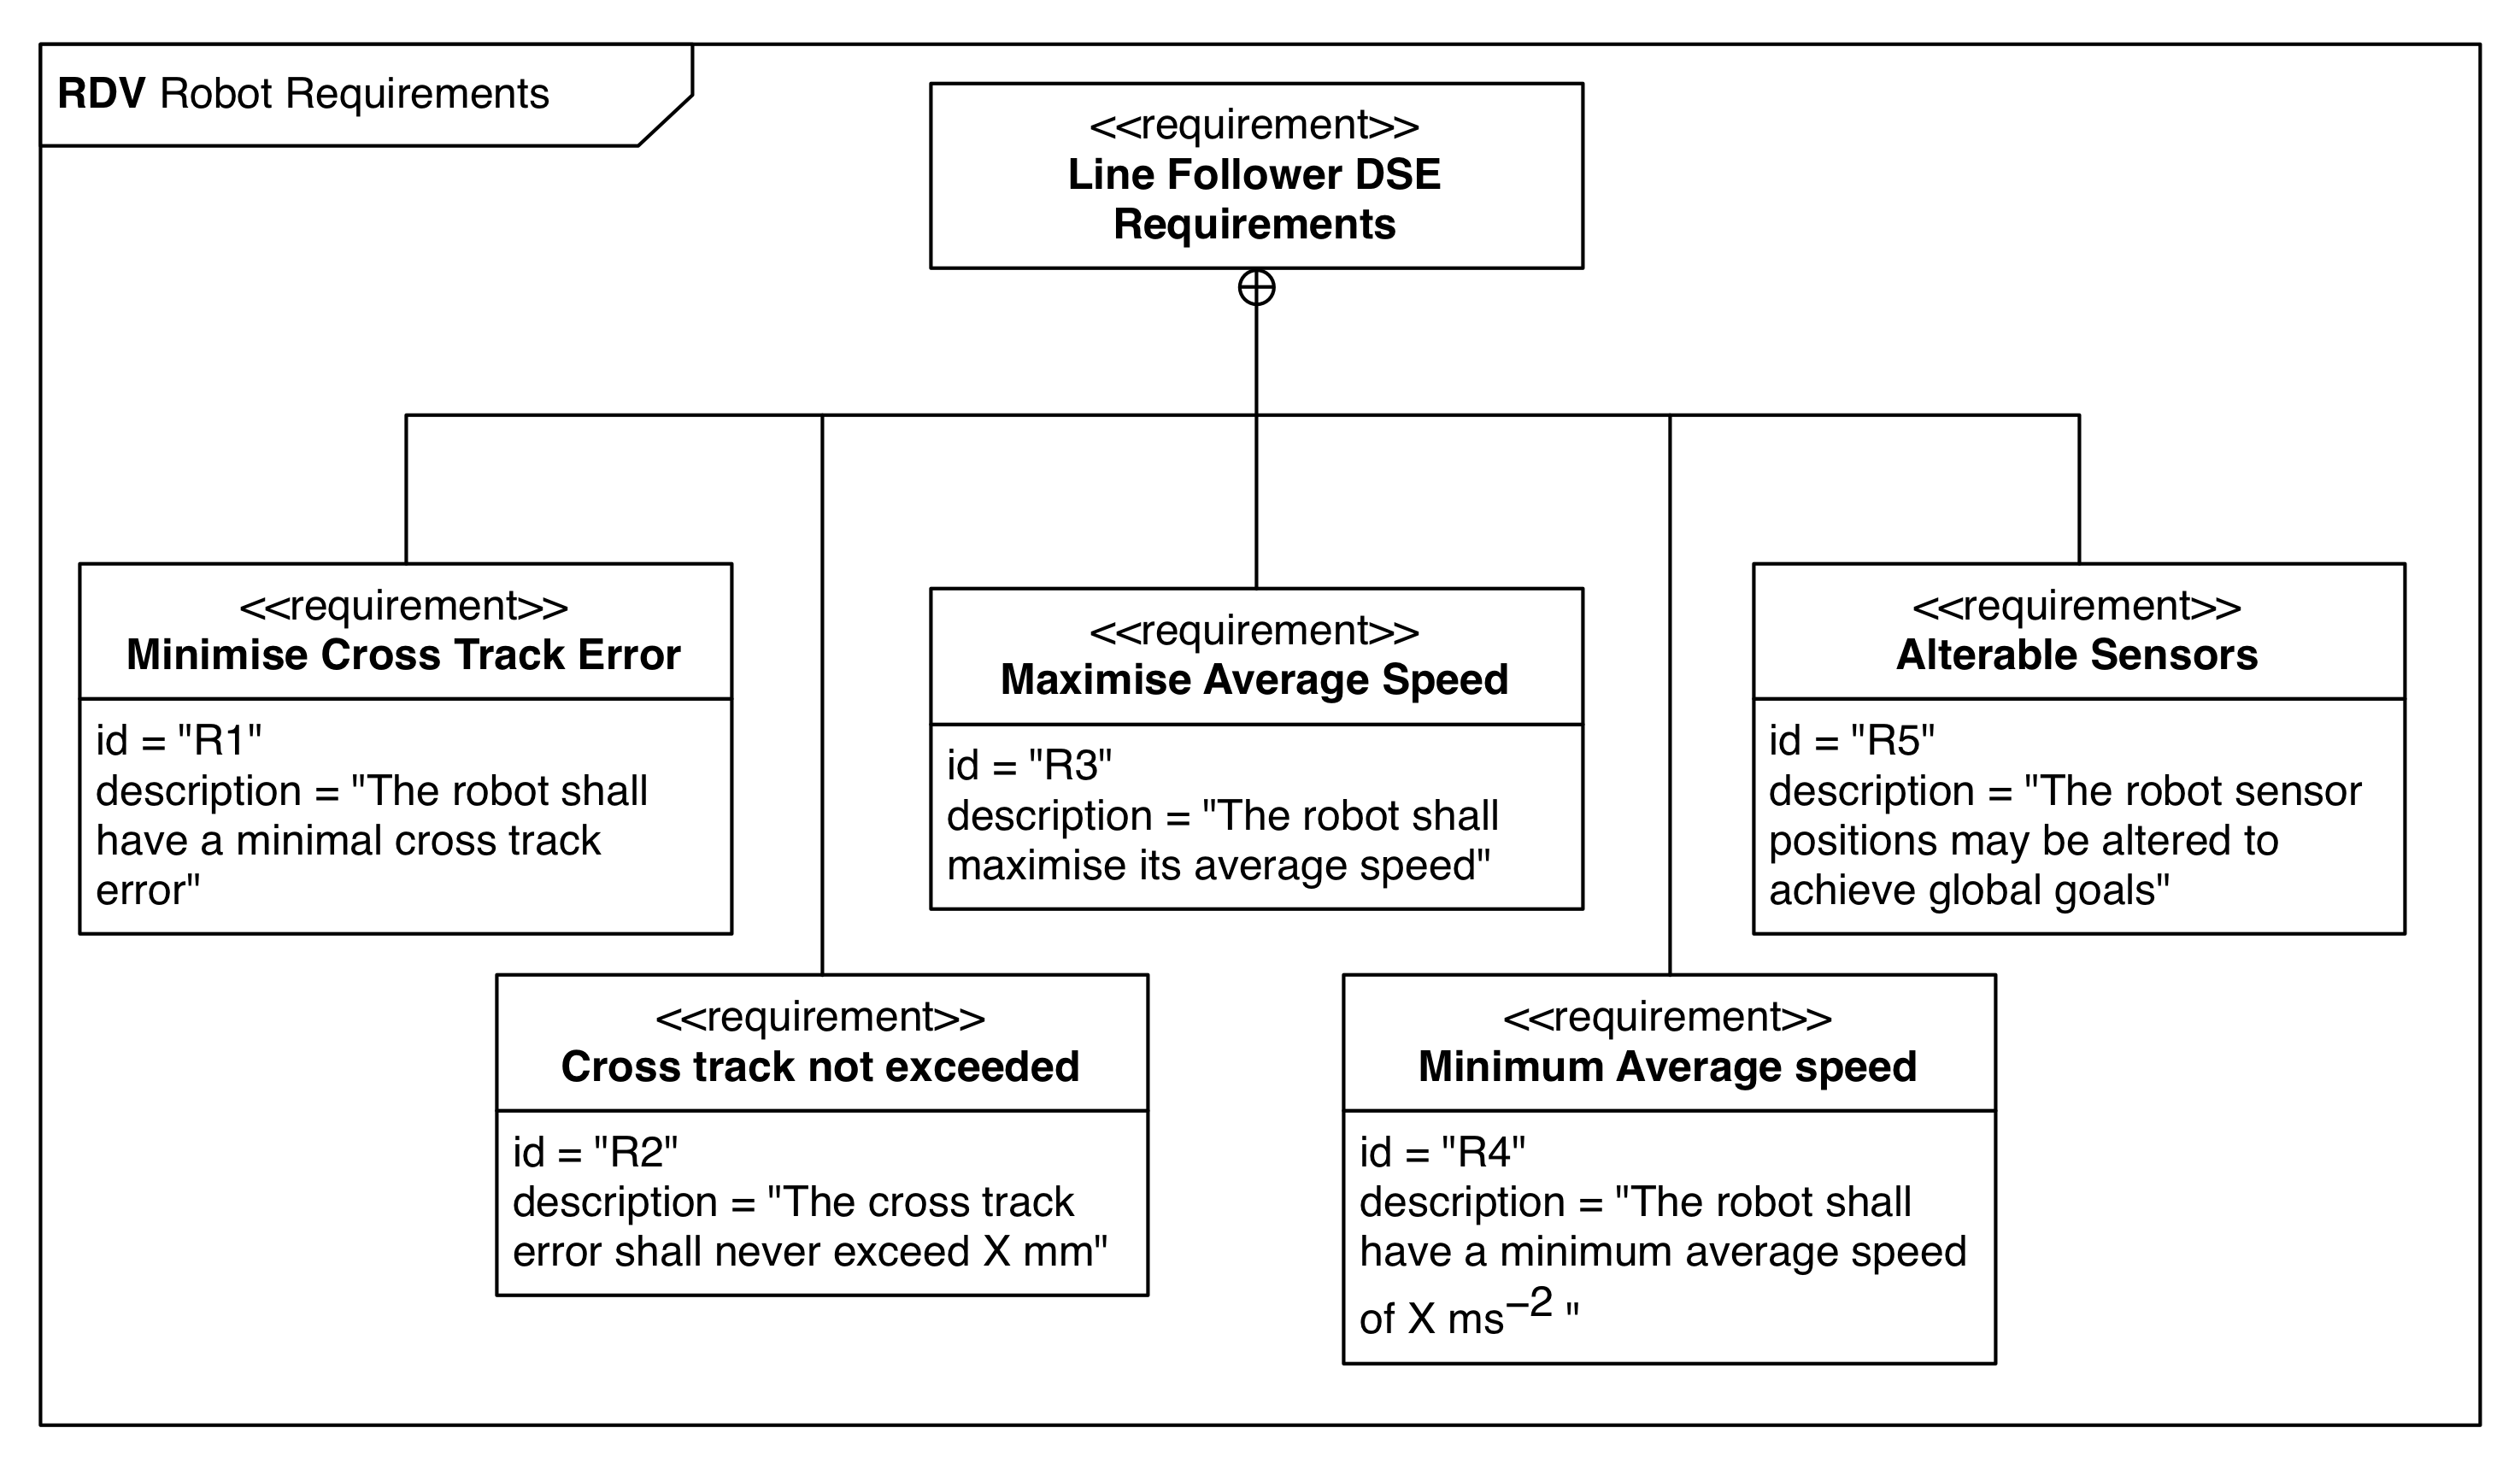
\includegraphics[width=0.8\textwidth]{figures/Robot_RDV}
\caption{Subset of the Requirements Definition View for requirements of the Line Following Robot}\label{fig:line_rdv}
\end{figure}


%\draftnote{Use appropriate requirements diagrams here}

\paragraph{Objectives from Requirements}

Based upon the requirements above, we define two objectives: the calculation of deviation from a desired path, and the speed of the robot.

\paragraph{Deviation}

The deviation from a desired path, referred to as the cross track error, is the distance the robot moves from the line of the map, as shown in Figure~\ref{fig:crossTrackError}.

\begin{figure}[htbp]
	\centering
	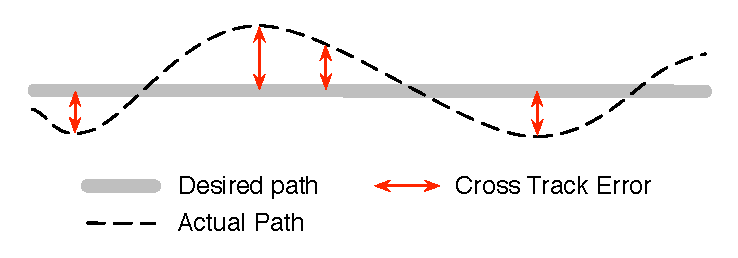
\includegraphics[scale=0.8]{figures/crossTrackError}
\caption{Cross track error at various points for a robot trying to follow a desired line}\label{fig:crossTrackError}
\end{figure}

To compute cross track error we need some model of the desired path to be followed and the actual path taken by the robot.  Each point on the actual path is compared with the model of the desired path to find its distance from the closest point, this becomes the cross track error.  If the desired path is modelled as a series of points, then it may be necessary to find shortest distance to the line between the two closest points.


%\paragraph{Range}



\paragraph{Speed}
The speed may be measured in several ways depending on what data is logged by the COE and what we really mean by speed, indicated in Figure~\ref{fig:robotSpeed}.

\begin{figure}[htbp]
	\centering
	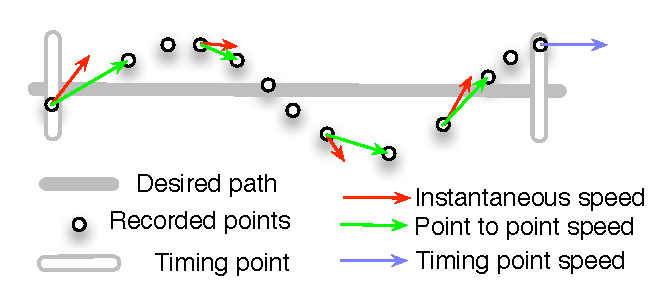
\includegraphics[scale=0.8]{figures/robotSpeed}
\caption{Cross track error at various points for a robot trying to follow a desired line}\label{fig:robotSpeed}
\end{figure}

Inside the CT model there is a bond graph flow variable that represents the forwards motion of the robot.  This variable is not currently logged by the COE but it could be and this would result in snapshots of the robot speed being taken when simulation models synchronise.  In this example, we take the view that speed is referring to the time taken to complete a lap.

%\paragraph{Longevity}

\paragraph{SysML Representation of Parameters, Objectives and Ranking}

We next consider the use of the upcoming DSE profile to define the DSE parameters, objectives and desired ranking function. In the following SysML diagrams, we explicitly refer to model elements as defined in the architectural model of the line follower study, presented in Deliverable D3.5~\cite{INTOCPSD3.5}.

\paragraph{Parameters}   In the requirements defined above, we see that the position of the line follower sensors may be varied. In real requirements, we may elicit the possible variables allowed. Figure~\ref{fig:dse_lfr_param} is a DSE Parameter Definition Diagram and defines four parameters required: \emph{S1\_X}, \emph{S1\_Y}, \emph{S2\_X} and \emph{S2\_Y}, each a set of real numbers.  The DSE experiment in this example is called \emph{DSE\_Example}.

\begin{figure}[htbp]
	\centering
	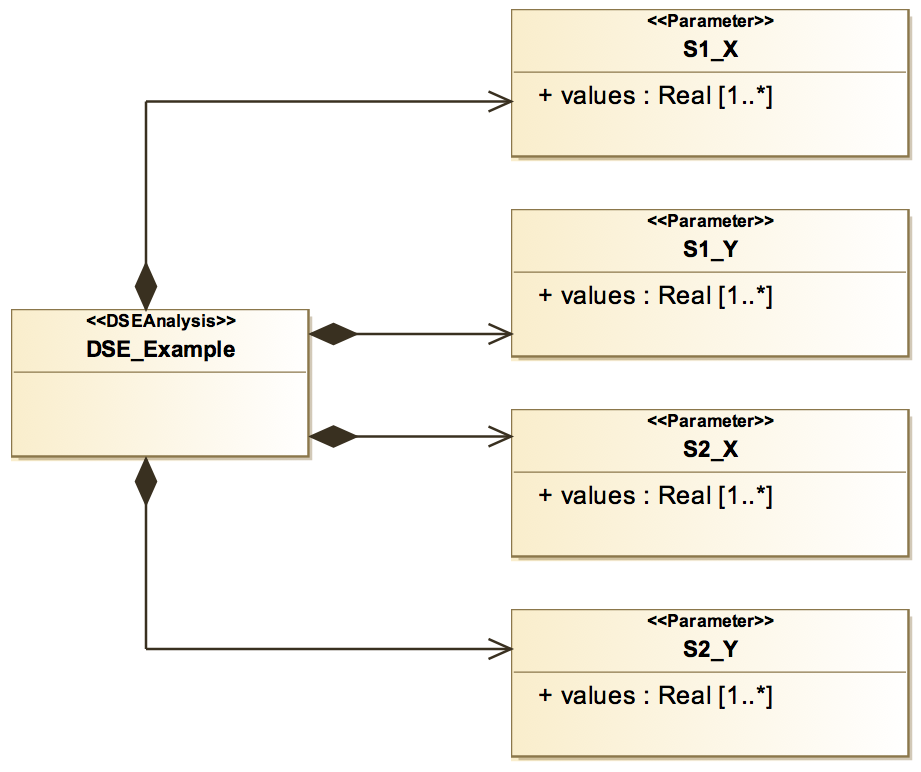
\includegraphics[width=0.7\textwidth]{figures/LFR_DSE_Param}
\caption{DSE-SysML Parameter Definition Diagram of Line Following Robot example}
\label{fig:dse_lfr_param}
\end{figure}

Figure~\ref{fig:dse_lfr_param2} identifies the architectural model elements themselves (the \texttt{lf\_position\_x} and  \texttt{lf\_position\_y} parameters of \emph{sensor1} and  \emph{sensor2}) and the possible values each may have (for example the \texttt{lf\_position\_x} parameter of \emph{sensor1} may be either $0.01$ or $0.03$). The diagram (or collection of diagrams if there is a large number of design parameters) should record all parameters for the experiment.

\begin{figure}[htbp]
	\centering
	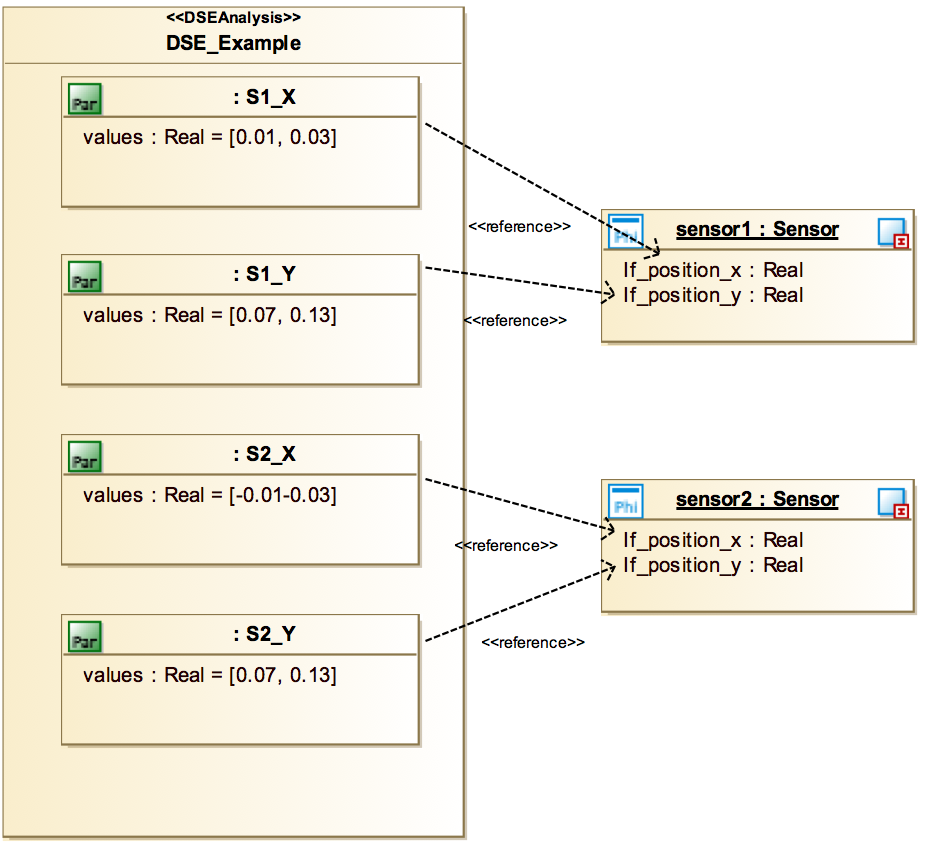
\includegraphics[width=0.7\textwidth]{figures/LFR_DSE_Param2}
\caption{DSE-SysML Parameter Connection Diagram of Line Following Robot example}
\label{fig:dse_lfr_param2}
\end{figure}

\paragraph{Objectives}    The objectives follow from the requirements as mentioned above. Figure~\ref{fig:dse_lfr_obj} shows the DSE Objectives Definition Diagram with four objectives:  \emph{meanSpeed}, \emph{lapTime}, \emph{maxCrossTrackError} and \emph{meanCrossTrackError}. Each have a collection of inputs -- defined either as constants (e.g. parameter \emph{p1} of \emph{meanSpeed}), or to be obtained for the multi-model.

\begin{figure}[htbp]
	\centering
	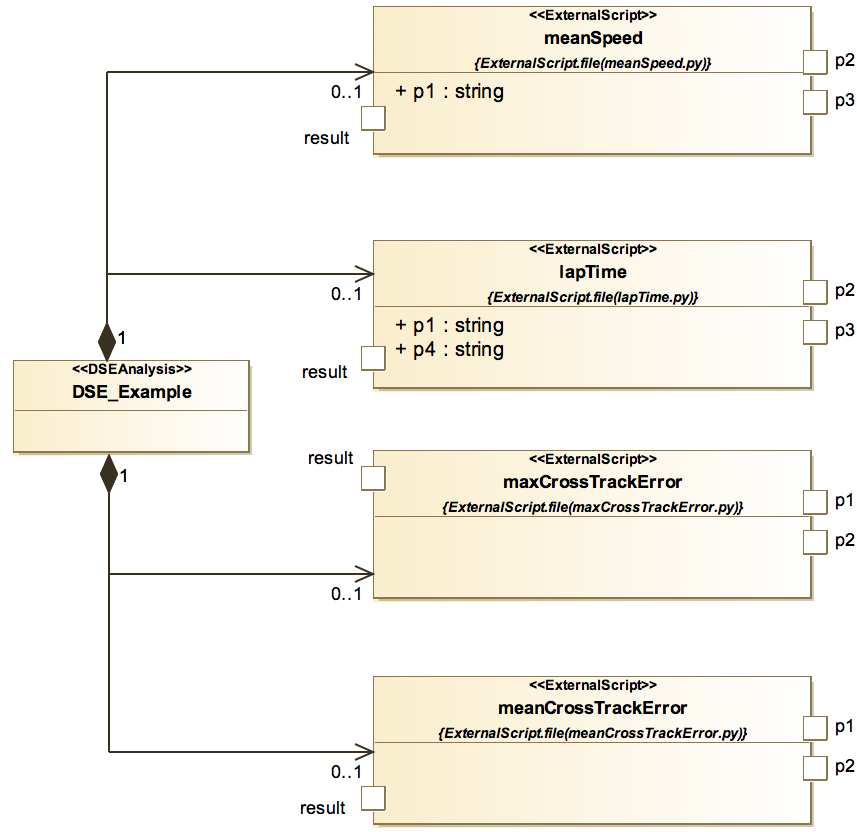
\includegraphics[width=0.7\textwidth]{figures/LFR_DSE_Obj}
\caption{DSE-SysML Objective Definition Diagram of Line Following Robot example}
\label{fig:dse_lfr_obj}
\end{figure}

The objective definitions are realised in Figure~\ref{fig:dse_lfr_obj2}. The \emph{meanSpeed} requires the step-size of the simulation (this is obtained from the co-simulation results, rather than defined here) and the \texttt{robot\_x} and \texttt{robot\_y} position of the robot body. The \emph{lapTime} objective requires the time at each simulation step (again, obtained directly from the co-simulation output), the \texttt{robot\_x} and \texttt{robot\_y} position of the robot body and the name of the map. Both the \emph{maxCrossTrackError} and \emph{meanCrossTrackError} objectives require only the \texttt{robot\_x} and \texttt{robot\_y} position of the robot body.

\begin{figure}[htbp]
	\centering
	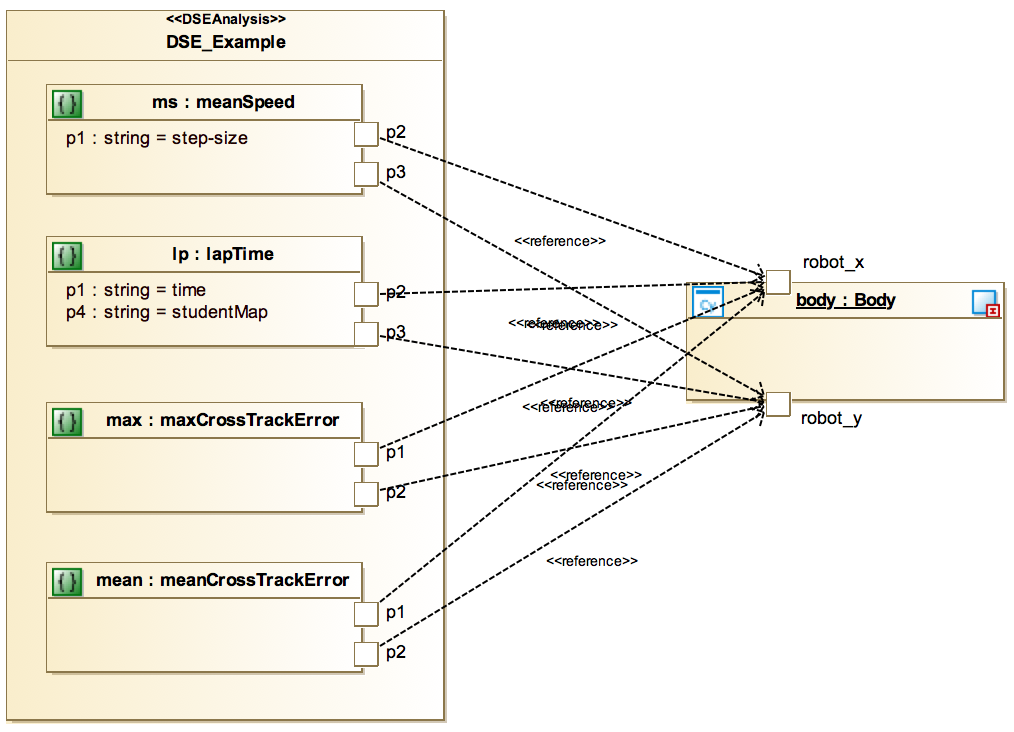
\includegraphics[width=0.7\textwidth]{figures/LFR_DSE_Obj2}
\caption{DSE-SysML Connection Objective Diagram of Line Following Robot example}
\label{fig:dse_lfr_obj2}
\end{figure}

\paragraph{Ranking} Finally, the DSE Ranking Diagram in Figure~\ref{fig:dse_lfr_rank} defines the ranking to be used in the experiment. This diagram states that the experiment uses the Pareto method, and is a 2-value Pareto referring to the \emph{lapTime} and \emph{meanCrossTrackError} objectives.

\begin{figure}[htbp]
	\centering
	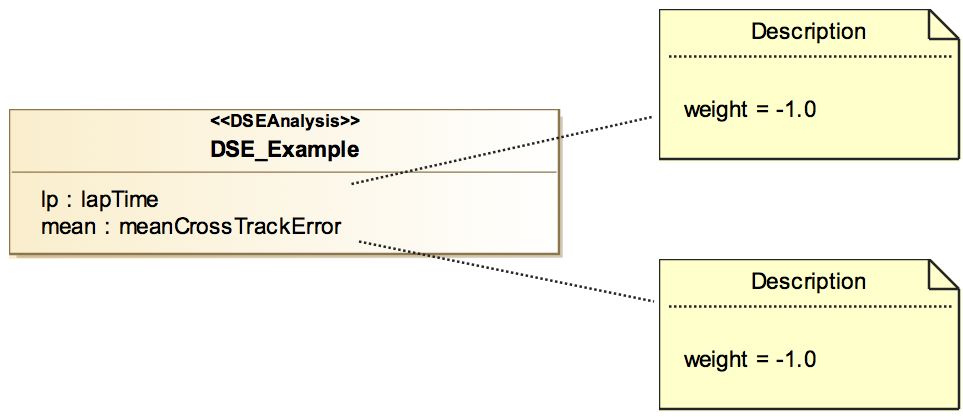
\includegraphics[width=0.6\textwidth]{figures/LFR_DSE_Rank}
\caption{Example DSE-SysML Ranking Diagram of Line Following Robot example}
\label{fig:dse_lfr_rank}
\end{figure}

\paragraph{DSE script}

%\draftnote{TWT: Please update this paragraph. Is this Modelio export available now?}

These diagrams may then be translated to the JSON config format required by the DSE tool.  The export of the configuration is performed in the Modelio tool and the subsequent movement of the resulting configuration file is performed in the INTO-CPS application (see the INTO-CPS User Manual, Deliverable D4.3a~\cite{INTOCPSD4.3a} for more details).  %At present this is a manual process, however tool support in Modelio is in preparation and shall be available early in Year 3 of the project. This tool support will provide the automated generation of a skeleton configuration, specifying the parameters, objectives and ranking to use. This leaves the choice of DSE algorithm and simulation timing settings for an engineer to specify in the INTO-CPS application.
Figure~\ref{fig:dse_config_json} shows the corresponding DSE configuration file for the line follower experiments. Note that where we refer to model elements of the architecture (such as model parameters), we now use the same conventions used in the co-simulation orchestration engine configuration.

\begin{figure}[h]
	\centering
	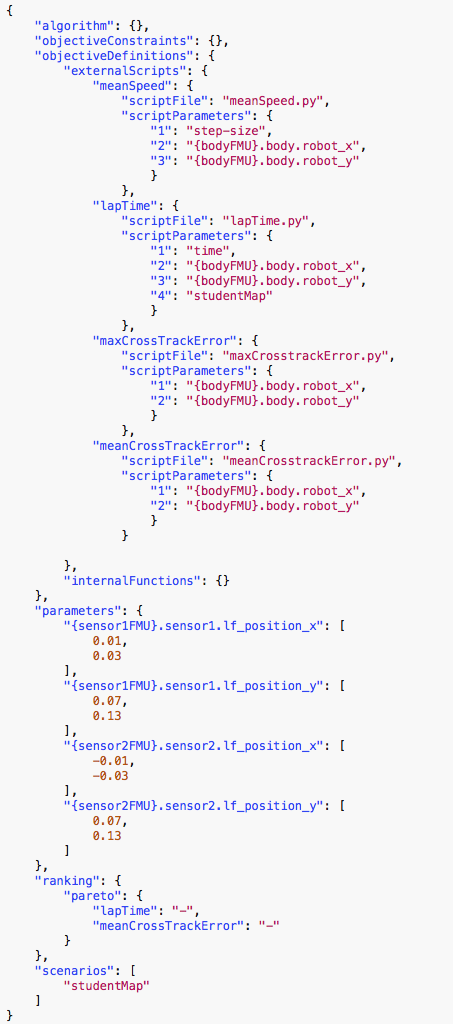
\includegraphics[scale=0.45]{figures/config-whole}
		\caption{A complete DSE configuration JSON file for the line follower robot example}
		\label{fig:dse_config_json}
\end{figure}

\paragraph{DSE results}

DSE is performed in the DSE tool (again, see the INTO-CPS User Manual, Deliverable D4.3a~\cite{INTOCPSD4.3a} for more detail) by processing the DSE configuration using scripts that contain the required algorithms.  The main scripts contain the search algorithm that determines which parameters to use in each simulation, the simplest of these is the exhaustive algorithm that methodically runs through all combinations of parameters and runs a simulation of each.  The log files produced by each simulation are then processed by other scripts to obtain the objective values defined in the previous section.  Finally, the objective values are used by a ranking script to place all the simulation results into a partial order according to the defined ranking.  The ranking information is used to produce tabular and graphical results that may be used to support decisions regarding design choices and directions.

Figure~\ref{fig:dse-results} shows an example of the DSE results from the line follower robot where the lap time and mean cross track error were the objectives to optimise.  These results contain two representations of the data, a graph plotting the objective values for each design, with the Pareto front of optimal trade-offs between the key objectives highlighted, here in blue. The second part of the results presents the data is tables, indexed by the ranking position of each result.  This permits the user to determine the precise values for both the measured objectives and also the design parameters used to obtain that result.

\begin{figure}[h!]
	\centering
	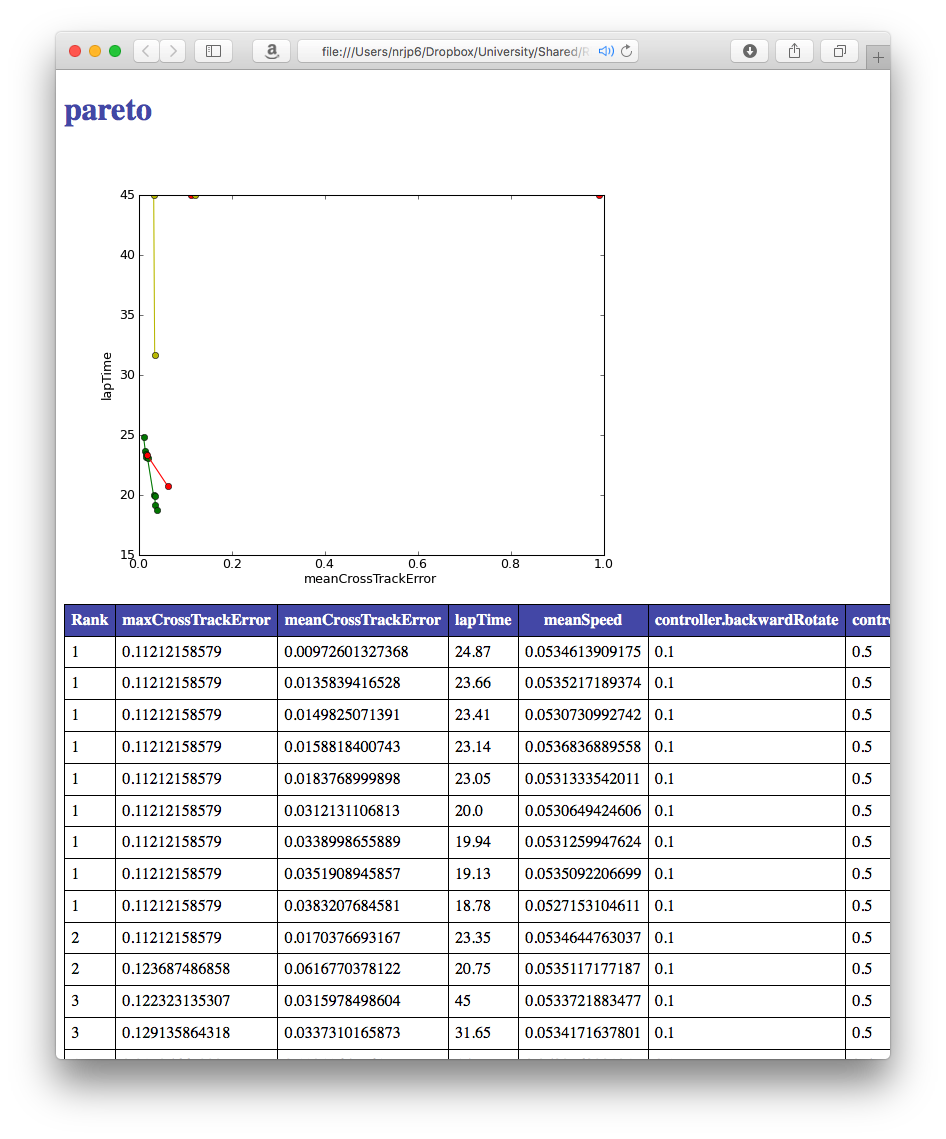
\includegraphics[width=0.9\textwidth]{figures/dse_results}
	\caption{DSE results}
	\label{fig:dse-results}
\end{figure}

\subsubsection{An Approach to Effective DSE}
\label{sec:dse-algorithms}

Given a ``designed'' design space using the method detailed above, we use the INTO-CPS Tool Chain to simulate each design alternative. The initial approach we took was to implement an algorithm to exhaustively search the design space, and evaluate and rank each design. Whilst this approach is acceptable on small-scale studies, this quickly becomes infeasible as the design space grows. For example, varying $n$ parameters with $m$ alternative values produces a design space of $m^n$ alternatives. In the remainder of this paper, we present an alternative approach to exploring the design space in order to provide guidance for CPS engineers on how to design the exploration of designs for different classes of problems.

\paragraph{A Genetic Algorithm for DSE}
Inspired by processes found in nature, genetic algorithms ``breed'' new generations of optimal CPS designs from the previous generation's best candidates. This mimics the concept of survival of the fittest in Darwinian evolution.
Figure~\ref{fig:ga_dse_process} represents the structure of a genetic algorithm used for DSE.  Several activities are reused from exhaustive DSE: simulation; evaluation of objectives; rank simulated designs; and generate results. The remaining activities are specific to the genetic approach and are detailed in this section.

\begin{figure}[h!]
	\centering
	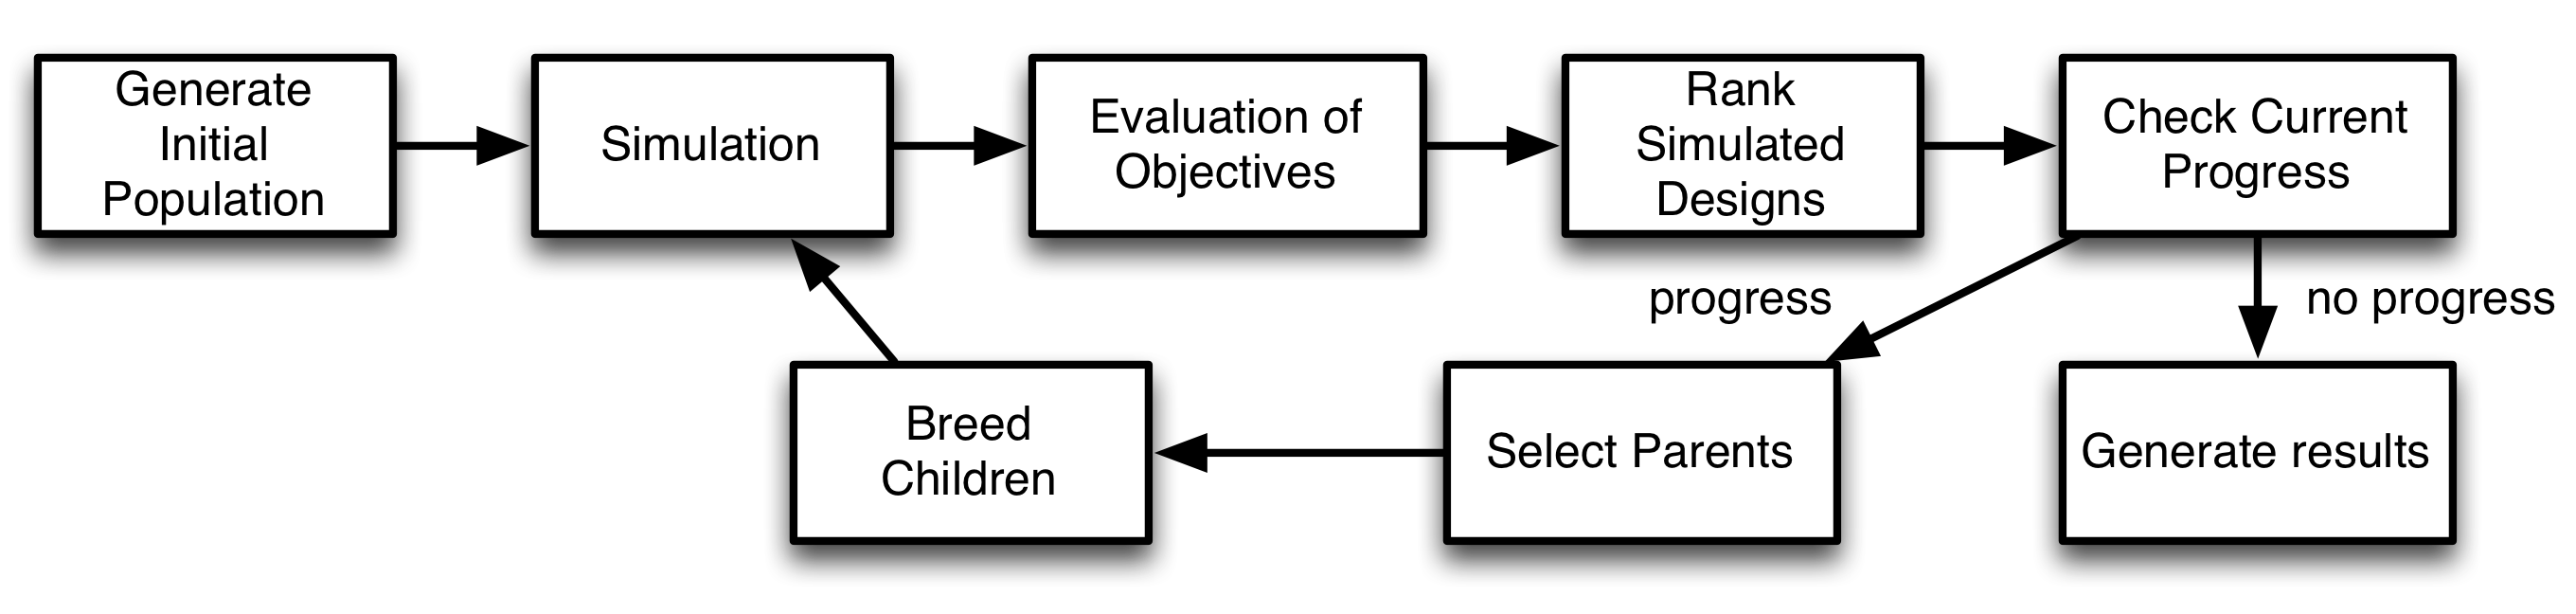
\includegraphics[width=0.9\textwidth]{figures/ga_process}
	\caption{High-level process for DSE Genetic Algorithm}
	\label{fig:ga_dse_process}
\end{figure}

\begin{description}
\item[Generating initial population:] Two methods for generating an initial population of designs are supported: randomly, or uniformly across the design space. Generating an initial design set which is distributed uniformly could allow parts of the design space to be explored that would otherwise not be explored with a random initial set. This could give us greater confidence that the optimal designs found by the genetic algorithm are consistent with the optimal designs of the total design space.
\item[Selecting parents:] Two options for parent selection are supported: random and distributed. Random selection means that two parents are chosen randomly from the non-dominated set (NDS). There is also a chance for parents to be selected which are not in the NDS, potentially allowing different parts of the design space to be explored due to a greater variety of children being produced.

%\draftnote{AI: Maybe we should put NDS in the glossary list}

An intelligent approach involves calculating the distribution of each design's objectives from other designs in the NDS. One of the parents chosen is the design with the greatest distribution, enabling us to explore another part of the design space which may contain other optimal designs. Picking a parent that has the least distribution suggests that this parent is close to other optimal designs, meaning that perhaps it is likelier to produce optimal designs.
		
Figure~\ref{fig:ga_fitness} shows the fitness roulette by which how much a design solution in Figure~\ref{fig:ga_fitness2} satisfies the requirements. It can be seen that there exists a relationship where the greater the fitness value a design has, the more likely it is to be selected as a parent. The probability $P$ of design d being selected as a parent can be calculated by:

\begin{figure}[htbp]
\centering
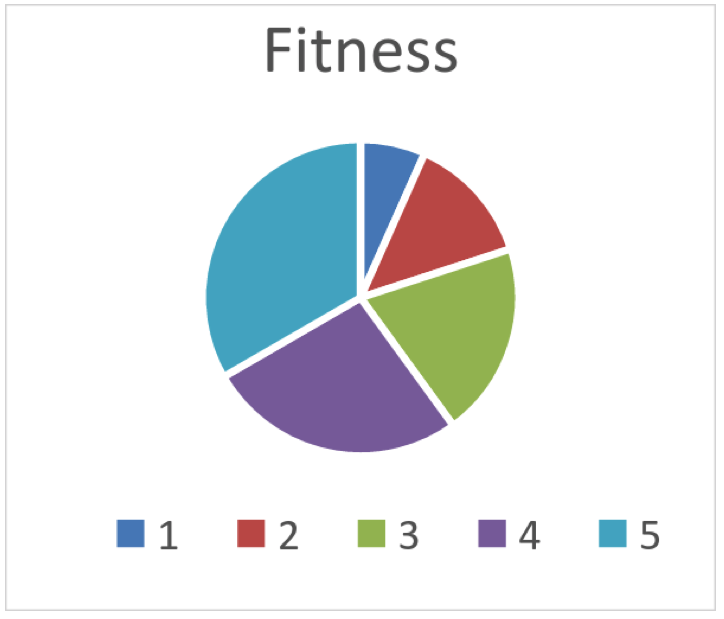
\includegraphics[width=0.25\textwidth]{figures/ga_fitness}
\caption{Example fitness roulette}
\label{fig:ga_fitness}
\end{figure}

\begin{figure}[htbp]
\centering
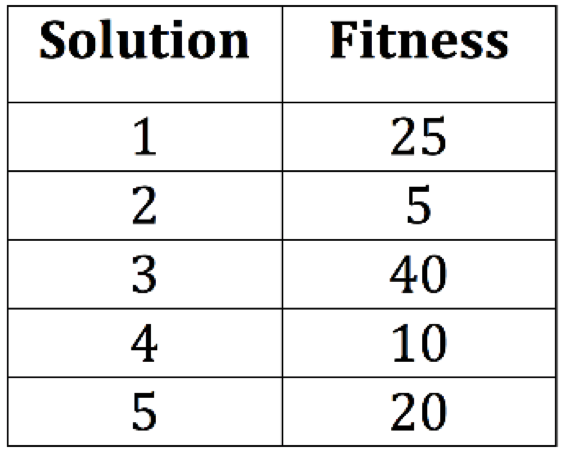
\includegraphics[width=0.25\textwidth]{figures/ga_fitness2}	
\caption{Genetic Algorithm fitness selection}
\label{fig:ga_fitness2}
\end{figure}


\item[Breeding children:] After the parents are selected, the algorithm creates two new children using a process of crossover. Figure~\ref{fig:ga_crossover} shows this process. Mutation could also occur, where a randomly chosen parameter's value is replaced by another value defined in the initial DSE configuration, producing new designs to explore other parts of the design space.

\begin{figure}[h!]
	\centering
	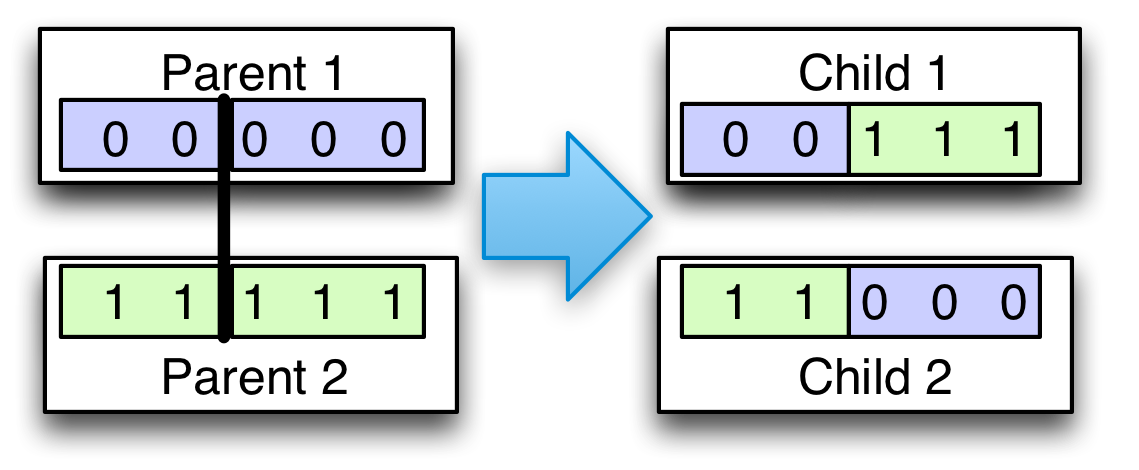
\includegraphics[width=0.45\textwidth]{figures/ga_breeding}
	\caption{Depiction of genetic crossover}
	\label{fig:ga_crossover}
\end{figure}

\item[Checking current progress:] Progression is determined by the change in the NDS on each iteration. It is possible to tune the number of iterations without progress before termination.

\end{description}
\paragraph{Measuring Effectiveness}
To provide guidance on selection and tuning of a specific algorithm to a DSE situation it is necessary that there is a means for experimenting with the algorithm parameters and also means for evaluating the resulting performance. To this end an experiment was devised that supports exploration of these parameters using a range of design spaces as the subject.
The experiment is based upon generating a ground truth for a set of design spaces such that the composition of each Pareto front is known and we may assess the cost and accuracy of the genetic algorithm's attempt to reach it. A limiting factor for these design spaces is that they must be exhaustively searched and so there are current four of these all based upon the line follow robot: an 81-point and a 625-point design space where the sensor positions are varied and a 216-point and 891-point design spaces where the controller parameters are varied.
There are three measures applied to each result that target the tension between trading off the cost of running a DSE against the accuracy of the result

\begin{description}
\item[Cost:] The simplest of the measures is the cost of the performing the search and here it is measured by the number of simulations performed to reach a result. For the purposes of comparison across the different design spaces, this cost is represented as a proportion of the total number of designs

$cost = \frac{|Simulations\ Run|}{|Design\ Space|}$

\item[Accuracy:] The ground truth exhaustive experiments provide us with the Pareto Front for that design space and each DSE experiment returns a non-dominated set of best designs found.  Here the accuracy measure considers how many of the designs in the genetic non-dominated set are actually the best designs possible. It is measured by finding the proportion of points in the genetic NDS that are also found in the ground truth Pareto front.

$accuracy = \frac{|GeneticNDS \cap ExhaustiveNDS|}{|GeneticNDS|}$

\item[Generational Distance:] The accuracy measure tells us something about the points in the genetically found NDS that are also found in the exhaustive NDS (Van Veldhuizen \& Lamont, 2000).  The generational distance gives us a figure indicating the total distance between the genetic NDS and the exhaustive NDS. It is calculated by computing the sum of the distance between each point in the genetic NDS and its closest point in the exhaustive NDS and dividing this by the total number of points.


$generational\ distance = \frac{\sqrt{(\sum_{i=1}^{n} d_{i}^{2})}}{n}$

\end{description}
\paragraph{Genetic DSE Experiments and Results}
The DSE experiments involved varying three parameters of the genetic algorithm and repeating each set of parameters with each design space five times.  The parameters of the genetic algorithm varied were:

\begin{description}
\item[Initial population size:] The initial population size took one of three values.  All design spaces were tested using an initial population of 10 designs, they were also tested with initial populations equal to $10\%$ of the design space and $25\%$ of the design space.  These are represented on the left hand graphs by the $10$, $10\%$ and $25\%$ lines.
\item[Progress check conditions:] The number of rounds the genetic algorithm would continue if there was no progress observed was tested with three values, 1, 5 and 10.  These are represented on the right hand graphs with the 1, 5 and 10 lines.

\item[Algorithm options:] There are two variants of the genetic algorithm, phase 1 with random initial population and random parent selection, and phase 3 which give an initial population distributed over the design space and where parent selection is weighted to favour diverse parents.  The phase one experiments are on the left hand side of the graphs, with points labelled `<design space size>-p1' while the phase three experiments are on the right labelled `<design space size>-p3'.
\end{description}

The results of the simulations are shown in graph form below.  Each point graphed is the averaged result of the five runs of each set of parameters.  Figure~\ref{fig:cost_ga_ex}, shows the graphs of cost of running the DSEs.  Encouragingly there is a slight trend of the cost of DSE reducing as a proportion of the design space as the design space size increases.  As expected the cost was greater with larger initial populations but the cost did not vary when changing the progress check condition as much as expected.

\begin{figure}[p]
	\centering
	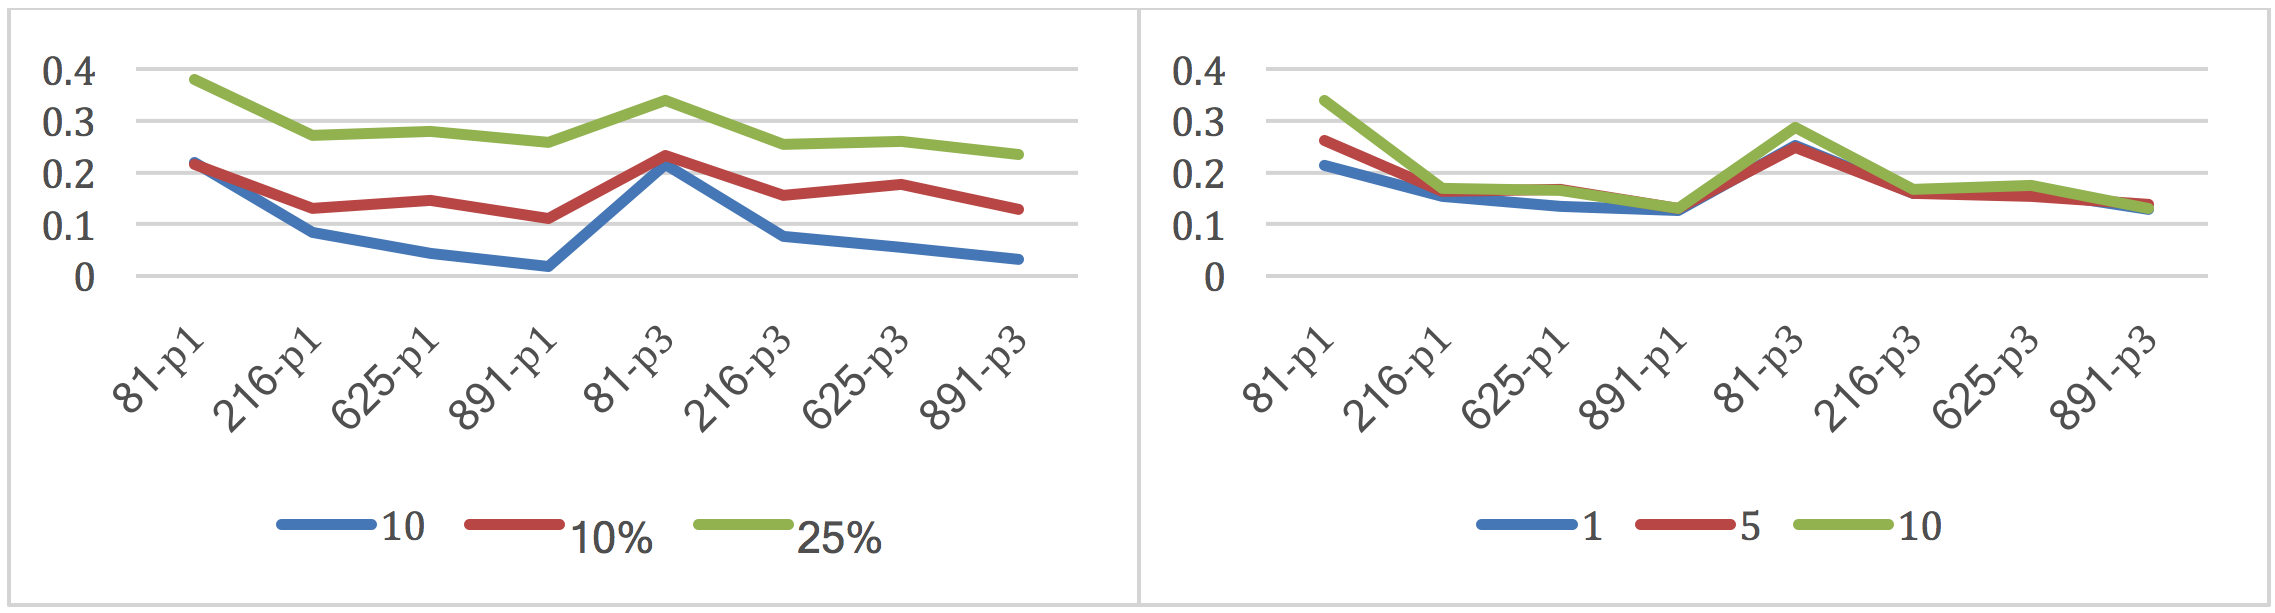
\includegraphics[width=1\textwidth]{figures/ga_cost}
	\caption{Cost of DSE, number of simulations run as proportion of the total design space.}
	\label{fig:cost_ga_ex}
\end{figure}
Figure~\ref{fig:acc_ga_ex} shows the graphs of DSE accuracy.  There is again a slight downward trend as design space size increases, meaning that there is a slight increase in the number of points in the genetic NDS that are not truly optimal.  As expected the larger initial population generally resulted in more accurate NDS, this was also true of using the largest value for the progress check condition.

\begin{figure}[p]
	\centering
	\includegraphics[width=1\textwidth]{figures/ga_accuracy}
	\caption{Accuracy of DSE, proportion of genetic NDS found in exhaustive NDS.}
	\label{fig:acc_ga_ex}
\end{figure}
Figure~\ref{fig:gap_ga_ex} presents the generational distance results.  Here we find that the results are generally low, with the exception of the 891-point design space which is significantly worse, the reason for this is still to be determined.  The largest initial design space resulted in the lowest (best) values as did using a progress check condition value of five.


\begin{figure}[p]
	\centering
	\includegraphics[width=1\textwidth]{figures/ga_distance}
	\caption{Gap between Genetic NDS and Exhaustive NDS.  The vertical axis has no meaningful units, a smaller number is better.}
	\label{fig:gap_ga_ex}
\end{figure}

\paragraph{Selecting Approaches based on Design Space}


The choice of which search algorithm to use when performing DSE is dependant on one factor, and that is a comparison of the 'simulations required' compared to the 'simulation budget',  before describing what to do with the comparison, it is first necessary to explain those terms.

The number of 'simulations required' is dependant on the number of different design alternatives that the DSE is supposed explore, but there also other factors, specifically repetitions and scenarios.  The 'design' part of the number of simulations required is determined by multiplying together the number of values each parameter may adopt, since this gives the number of unique designs.  If the DSE configuration includes parameter constraints then the number of valid designs will be lower since some parameter combinations will fail to meet the constraints.  For example, A line follower robot with two sensors, where each sensor has three possible x position values and three possible y position values, would have a design space size of 81, however if those parameters are constrained so designs must be symmetrical, i.e. the x and y values of each sensor must be identical, then the design space only has nine points.

If a simulation model contains random elements, such a noisy inputs to sensors or models of dropped messages on a network, then this leads to the simulation results being non-deterministic.  In this case, it will be necessary to perform repeated simulations of the same design with the same starting conditions to account for the random variation.

'Scenarios' refer to the environment around the actual system-under-test in the simulation, for example, in the case of a line following robot, the environment could include the map that the robot is to follow along with other factors such as the intensity of the ambient light.  If there is a desire to perform simulations under different scenarios, then the number of scenarios must also be taken into account when determining the required number of simulations.  The final required number of simulations then is the product of the design space size, the number of repetitions and the number of scenarios.

The simulation budget term refers to the maximum number of simulations that a user may perform as part of DSE experiment.  It is a matter for the user to determine the value for this budget, but it could be determined by determining the amount of CPU time allocated to the DSE and dividing it by the time to run a simulation and compute the objective values.


The decision of whether to use the exhaustive search algorithm or a closed loop search can be made by comparing the number of simulations required with the simulation budget.  If the simulation budget is greater than or equal to the required number of simulations, then an exhaustive search should be used as this guarantees to find the optimal designs given the design parameter values, if the budget is less than the required number of simulations required then a closed loop approach is needed.

\paragraph{Parameters for a Genetic Search}

If the decision is made to perform a genetic search, then it is important to note that there are two parameters that affect how the algorithm behaves and will have an effect on the outcome.  The first of these parameters is the initial population size, this defines how many random designs are generated at the start of the search as a seed for the process.  A general rule for this initial population size is that it should be 10 times the number of dimensions (parameters)~\cite{diaz07initial}, with the caveat that as the number of dimensions increases, this multiplier must also also increase.

The second parameter is the termination condition, or the number generations the algorithm will continue without seeing progress before it terminates.  The genetic algorithm measures progress by looking at the designs that make up the non-dominated set of the Pareto analysis.  The only way membership of this set can change between two generations is if better designs, according to the objective measures, have been found, so if membership changes then the search is making progress towards finding better designs.  It is not unusual for the algorithm to breed new designs that are not better than those currently in the non-dominated set and so to have a generation that does not show progress, but then to make progress in a subsequent generation.  Thus, the number of generations without progress parameter is used to relax the termination condition to permit generations without progress without stopping.  Increasing this value will increase the probability that the search will not become stuck in some local optima in the results and may progress to find better designs.  There is a cost associated with increasing this value since, as the algorithm produces two new designs per generation, there will be two times the number of generations without progress simulations run at the end of the process that do not lead to better results~\cite{Fitzgerald&17a}.


%\draftnote{CJG: Basic rule, if you can perform exhaustive... do}


\paragraph{Iterative Exhaustive Search}

An alternative to the genetic search, which is automated, is to use repeated exhaustive searches to home in on better regions of the design space.  In this approach the user would plan to perform multiple DSE experiments, each using some portion of their total simulation budget.  The first DSE experiment is used to cover the whole range of the design space, but not including all values for each parameter.   In this way the first DSE is used to locate regions of interest within the design space.  The regions of interest are areas of the design space that produced the better designs according to the ranking results, with the bounds of the 'area' defined by the parameter values that produced good results. The user then divides up their remaining simulation budget between the one or more areas of interest and perform further DSE on those areas.  Figure~\ref{fig:dse:iterative1} shows an example initial search, with the blue dots indicating simulations performed and the green areas giving the best results.  The user then divides their remaining simulation budget among the three green areas of interest, searching each with a higher resolution in an attempt to extract the best results from each, Figure~\ref{fig:dse:iterative2}.

\begin{figure}[p]
	\centering
	
	%\begin{subfigure}[t]{0.45\textwidth}
	\includegraphics[width=0.35\textwidth]{figures/Traceability/IterativeStep1}
	\caption{Step 1 of an iterative search.  The best results being found in the green regions}
	\label{fig:dse:iterative1}
	%\end{subfigure}
\end{figure}

\begin{figure}[p]
	\centering
	\includegraphics[width=0.35\textwidth]{figures/Traceability/IterativeStep2}
	\caption{Step 2 of an iterative search.  The green regions are searched with a higher resolution to find the best results}
	\label{fig:dse:iterative2}
\end{figure}

